%  Main document of Paul Hein's MS Thesis  %
%            for use with the              %
%  University of Arizona Thesis Class,     %
%               uathesis.cls               %
%------------------------------------------%

% There are five copyright options.  Copyright, no copyright, and three
% different Creative Commons licences.  Use the one you want (If you go
% Creative Commons, I (DM) think the CC-BY-ND makes the most sense)  See
% uathesis.cls for the reason why the non-commercial licenses are not
% included.

%\documentclass[dissertation,copyright]{uathesis}
%\documentclass[dissertation,CC-BY]{uathesis}
%\documentclass[dissertation,CC-BY-SA]{uathesis}
% \documentclass[dissertation,CC-BY-ND]{uathesis}
%\documentclass[dissertation,generatedon]{uathesis}
\documentclass[thesis]{uathesis}

% Package Usage
% These are the packages that we need
%\usepackage{algorithm}
%\usepackage{algorithmic}

% \usepackage[ruled,boxed,noend]{algorithm2e}
\usepackage{graphicx}
\usepackage[caption=false]{subfig}
\usepackage{natbib}
% natbib is available on most systems, and is terribly handy. If you want to use a different Bibliography package, you should be able to, just change this and the \bibliographystyle command below. Be warned that you may need to do a little hacking to get the REFERENCES item to show up in your TOC.

% Compatibility with the AASTEX package of the American Astronomical Society.
%\usepackage{deluxetable}		% Allows use of AASTEX deluxe tables
%\usepackage{aastex_hack}		% Allows other AASTEX functionality.

% These are other packages that you might find useful.
% For controlling the fonts, see http://www.math.uiuc.edu/~hartke/computer/latex/survey/survey.html

% The following is a nice font set:
%\usepackage{mathtime}			% Times for letters; Belleek math.
%
%\usepackage{amsmath}			% AMS Math (advanced math typesetti`ng)
%\usepackage{lscape}			% Used for making fitting large tables in by putting them landscape
%\usepackage{refs}

% PACKAGES ADDED BY PAUL HEIN
\usepackage{microtype}
\usepackage{tikz}
\usetikzlibrary{bayesnet}

\usepackage{placeins}
\graphicspath{ {mainmatter/figs/} }

\usepackage{amssymb}
\usepackage{amsmath}
\usepackage{amsfonts}
\usepackage{algorithm}
\usepackage[noend]{algpseudocode}
\usepackage[T1]{fontenc}
\MakeRobust{\Call}

% If you are using hyper-ref (recommended), this command must go after all
% other package inclusions (from the hyperref package documentation).
% The purpose of hyperref is to make the PDF created extensively
% cross-referenced.
\usepackage[bookmarks,colorlinks=true,urlcolor=black,linkcolor=black,citecolor=black]{hyperref}

% Set up some values.
\completetitle{A Framework for Automating Scientific Software Model Analysis}
\fullname{Paul Douglas Hein} % Grad college wants your full name here.
\degreename{Master of Science}	% Title of your degree.

\newcommand{\ctm}[1]{\textcolor{teal}{#1}}

\begin{document}

% Set up the title page
\maketitlepage
{DEPARTMENT OF COMPUTER SCIENCE}	% Title of your department.
{2019}

% Insert the approval form.
\approval
{3 June 2019}		% Defense Date
{Clayton Morrison}		% Dissertation Director
{Mihai Surdeanu}		% 1st committee member
{Richard Snodgrass}		% 2nd committee member
{Associate Professor}
{School of Information}

% Include the ``Statement by Author'' for Dissertations
% NOTE: Apparently I only need this if I want to file for copyright
% \statementbyauthor[Clayton T. Morrison\\Professor of Information]

% Include the ``Acknowledgements''
% NOTE: Only need this if I need to acknowledge any one or any group
% TODO: Ask Clay if I should acknowledge anyone (maybe UA HPC or some group members?)
% \incacknowledgements{acknowledgements}

% Include the ``Dedication''
% NOTE: Don't need this and don't think it's warranted
% \incdedication{dedication}

\tableofcontents        % Create a ``Table of Contents''
\listoffigures          % Create a ``List of Figures''
% \listoftables           % Create a ``List of Tables''
\incabstract{abstract}  % Include the ``Abstract''

% Include the various chapters
\chapter{INTRODUCTION\label{chapter:introduction}}
The nature of scientific models is a deep philosophical topic \citep{giere2010explaining}, \citep{morrison2009models}, \citep{frigg2006models}.
For the purposes of this thesis, we consider a family of abstracted scientific models as assertions about a collection of variables that refer to aspects of the world, along with a set of functional relations between variables that stipulate how the state of one variable is a function of zero or more other variables. We refer to these as {\em executable} models. Executable models specify enough detail such that given values of input variables, the model can calculate the state of all of the other variables of the model.
This form of model can be represented as a graph, such as that illustrated in Figure~\ref{fig:example_sci_model}, where variables (ovals) are connected to one another by functions (boxes) that determine how variables influence each other.
As illustrated in the figure, models like these can be used to study real-world systems by making a claim (potentially directly testable) about how different observed states of the world are causally related: the executable model asserts that states of parent (input) variables will (partially) determine the states of child (output) variables as according to the function between the variables.
Additionally, uncertainty in variables can be represented explicitly by an empirical or estimated distribution over variable values. For example, the empirical distribution over {\tt Total Daily Rainfall} in Fig~\ref{fig:example_sci_model} is used to characterize the uncertainty in the {\tt Water} input variable to the model.
Using the functions included in the model that describe how variables effect each other, the uncertainty imposed upon the inputs then induces a distribution over output variables of the model: In Fig.~\ref{fig:example_sci_model} (which has only one output variable), this is seen in the distribution over predicted {\tt Crop Yield} values, which is a direct result of the uncertainty in amount of {\tt Water} present.

\begin{figure}[!htbp]
  \centering
  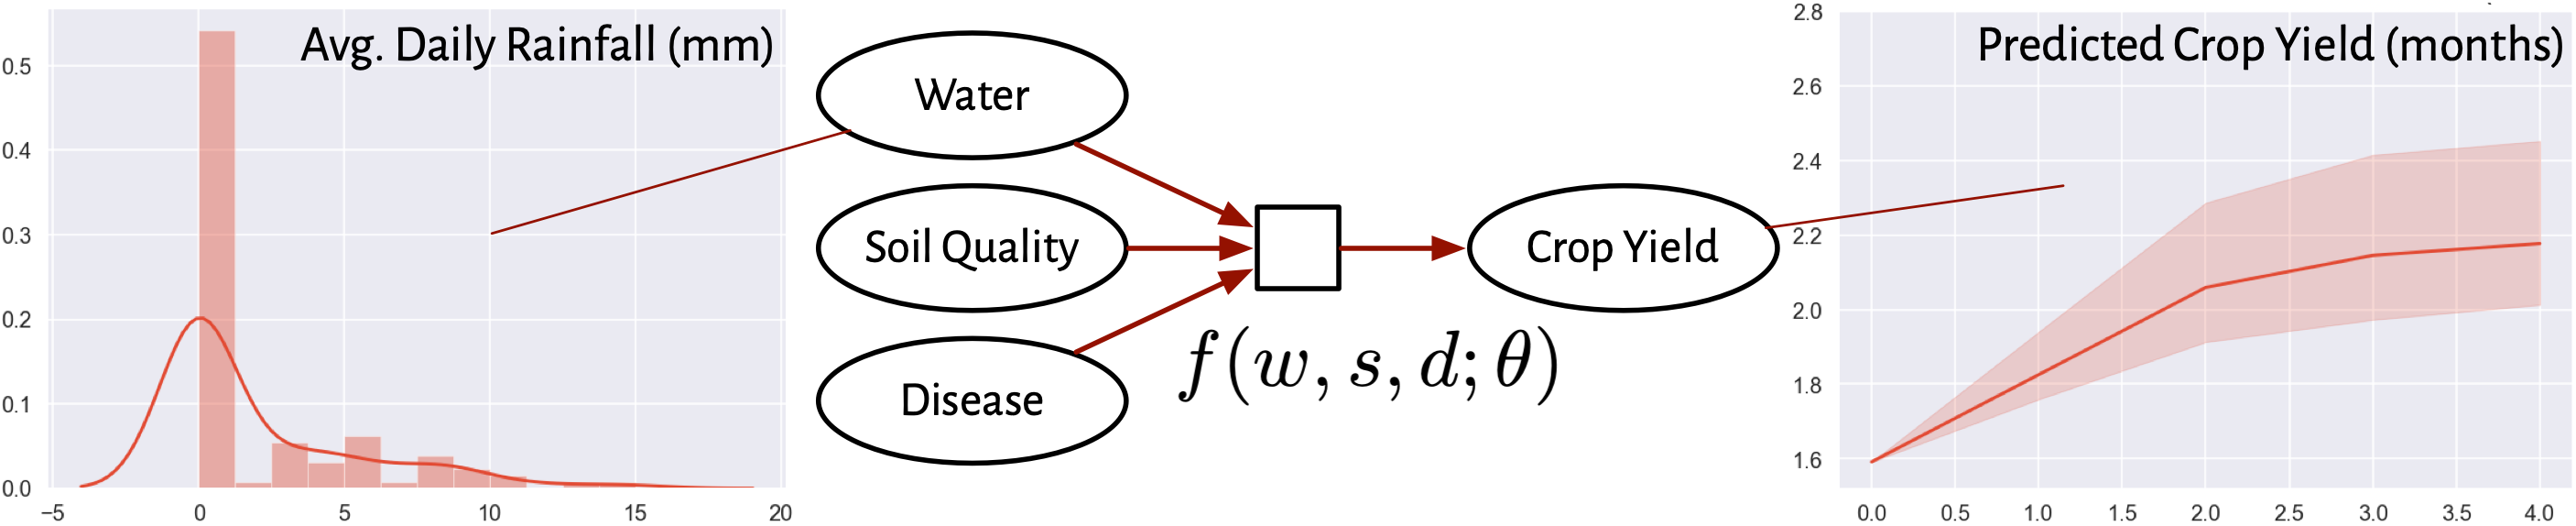
\includegraphics[width=\textwidth]{example_executable_model}
  \caption[Example of a Scientific Model]{An illustration of an executable model that shows how a distribution over a model input can be used to make predictions about the models output. In this function node of this model \textit{w, s, d} represent model inputs and $\theta$ represents the collection of model parameters.}
  \label{fig:example_sci_model}
\end{figure}

Translating knowledge about the uncertainty present in the inputs of a scientific model into a statement about the uncertainty in the model's output gives domain modelers an incredibly useful tool: the ability to make predictions along with a basis for assessing our confidence in the predictions.
Not only are scientific models able to make predictions, but the structure of the functional relations among variables allows those predictions to be interpreted and explained.
Consider the following question that could be posed to a team of domain modelers:
\begin{quote}
\textit{Will South Sudan be able to generate and deliver enough food to its population over the next three years?}
\end{quote}
At its core, this question is asking domain modelers to make a prediction about the state of several real-world variables.
For this example, domain modelers need to be able to make predictions about the expected food production, the expected population size, and the expected security of food transportation networks of South Sudan for the next three years.
The importance of this question also dictates that the predictions proposed by the domain modelers comes with an interpretable explanation that accounts for why the predictions are what they are.
Domain modelers can design a scientific model to answer each of the component questions included in the overall question, where each model provides an explainable prediction.
This ability to make explainable predictions, such as the ones necessary to answer important questions including the one above, has particularly led to the increased adoption of executable models by the scientific community for studying complex systems.

\section{Motivation\label{sec:motivation}}
The use of executable models has lead to the development of many supporting tasks that are carried out by \emph{domain modelers}, the scientists who seek to use models in their research studying a specific domain.
In general, science is driven by the repeated process of proposing multiple different, competing models of how observable phenomena may work.
A simple example of such a situation is illustrated in Figure~\ref{fig:simple_crop_CAG}, which depicts two competing models, each of which seeks to describe how the yield of a particular crop is affected by changes in the amount of rain and soil water absorption rate over time (expressed in \emph{Day}s).

\begin{figure}[!htbp]
  \centering
  \tikz{ % Simple Crop Yield model example
    \tikzstyle{readable}=[rectangle, thick, rounded corners]
    \node[latent, readable] (crop_yield) {$Yield$} ; %
    \node[latent, readable, above=of crop_yield] (total_rain) {$Rain_{total}$} ; %
    \node[latent, readable, above=of total_rain] (rain) {$Rain$} ; %
    \node[obs, readable, above=of rain] (max_rain) {$Rain_{max}$} ; %
    \node[obs, readable, left=of max_rain] (absorption) {$Absorption$} ; %
    \node[obs, readable, right=of max_rain] (consistency) {$Consistency$} ; %
    \node[obs, readable, right=of rain] (day) {$Day$} ; %
    \edge {day, consistency, absorption, max_rain} {rain} ; %
    \edge {rain} {total_rain} ; %
    \path [->] (total_rain) edge  [loop right] (total_rain);
    \edge {total_rain} {crop_yield} ; %

    \plate {loop} {(rain)(day)(total_rain)} {$Day$} ;
  }
  \tikz{ % Different Crop Yield model example
    \tikzstyle{readable}=[rectangle, thick, rounded corners]
    \node[latent, readable] (crop_yield) {$Yield$} ; %
    \node[latent, readable, above=of crop_yield] (total_rain) {$Rain_{total}$} ; %
    \node[latent, readable, above=of total_rain] (rain) {$Rain$} ; %
    \node[obs, readable, above=of rain] (max_rain) {$Rain_{max}$} ; %
    \node[obs, readable, right=of max_rain] (absorption) {$Absorption$} ; %
    \node[obs, readable, left=of rain] (consistency) {$Consistency$} ; %
    \node[obs, readable, left=of total_rain] (sunlight) {$Sunlight$} ; %
    \node[obs, readable, right=of rain] (day) {$Day$} ; %
    \edge {day, absorption, max_rain} {rain} ; %
    \edge {rain, consistency} {total_rain} ; %
    \path [->] (total_rain) edge  [loop right] (total_rain);
    \edge {total_rain, sunlight} {crop_yield} ; %

    \plate {loop} {(rain)(day)(total_rain)} {$Day$} ;
  }
  \caption[Competing Models of Crop Yield]{Two competing scientific models depicting the effects of rain on the yield of a crop over a span of days given a set of input variables (shaded). We see that the two models share many of their inputs but that some inputs may not be shared and the wiring of the inputs to the output variable differs between the two models.}
  \label{fig:simple_crop_CAG}
\end{figure}

We can see that, while the two models shown in the figure share several variables, some variables are not shared and the directed edges in the two models, representing how one variable’s state is a function of other variable(s), is not identical.
Each of these models makes a different set of claims about how the state of \emph{Yield} is determined by other states of the world.
A critical task of scientific reasoning is to determine which model is a better description of how nature works (or the possibility that neither is a good account).
This is an example of the general task of \textit{model choice}.
The model choice task requires domain modelers to analyze the available competing models of their system of interest and then to select which model best describes the outcomes of experiments or other observations.

Another, closely related task is \emph{model analysis}.
In model analysis, properties of an executable model are studied, such as how sensitive variations in output variables are to changes in input variables.
For example, in the case of the comparative crop yield examples shown in Figure~\ref{fig:simple_crop_CAG} domain modelers may use model analysis to measure the comparative uncertainty of the output of each model that is caused by {\tt Absorption}.

Similar to how multiple competing models of the same real-world systems exist, there are also models for different aspects of real-world systems that interact with one another.
Accounting for crop yield as a function of soil, water and disease is just a small part of a much larger set of interacting processes that include the impact of climate on the presence of water and other growing conditions, as well as how the yield impacts local and global economics. A model of crop yield should be composed with other models of related real-world systems to form an aggregate model that now links the interactions between a larger set of world states.
This is the task of \textit{model composition}.
Figure~\ref{fig:composition_example} presents a ``map'' of the relationships between families of models (colored regions) that describe a number of different aspects of the world that are all involved in predicting and understanding food security.

\begin{figure}[!htbp]
  \centering
  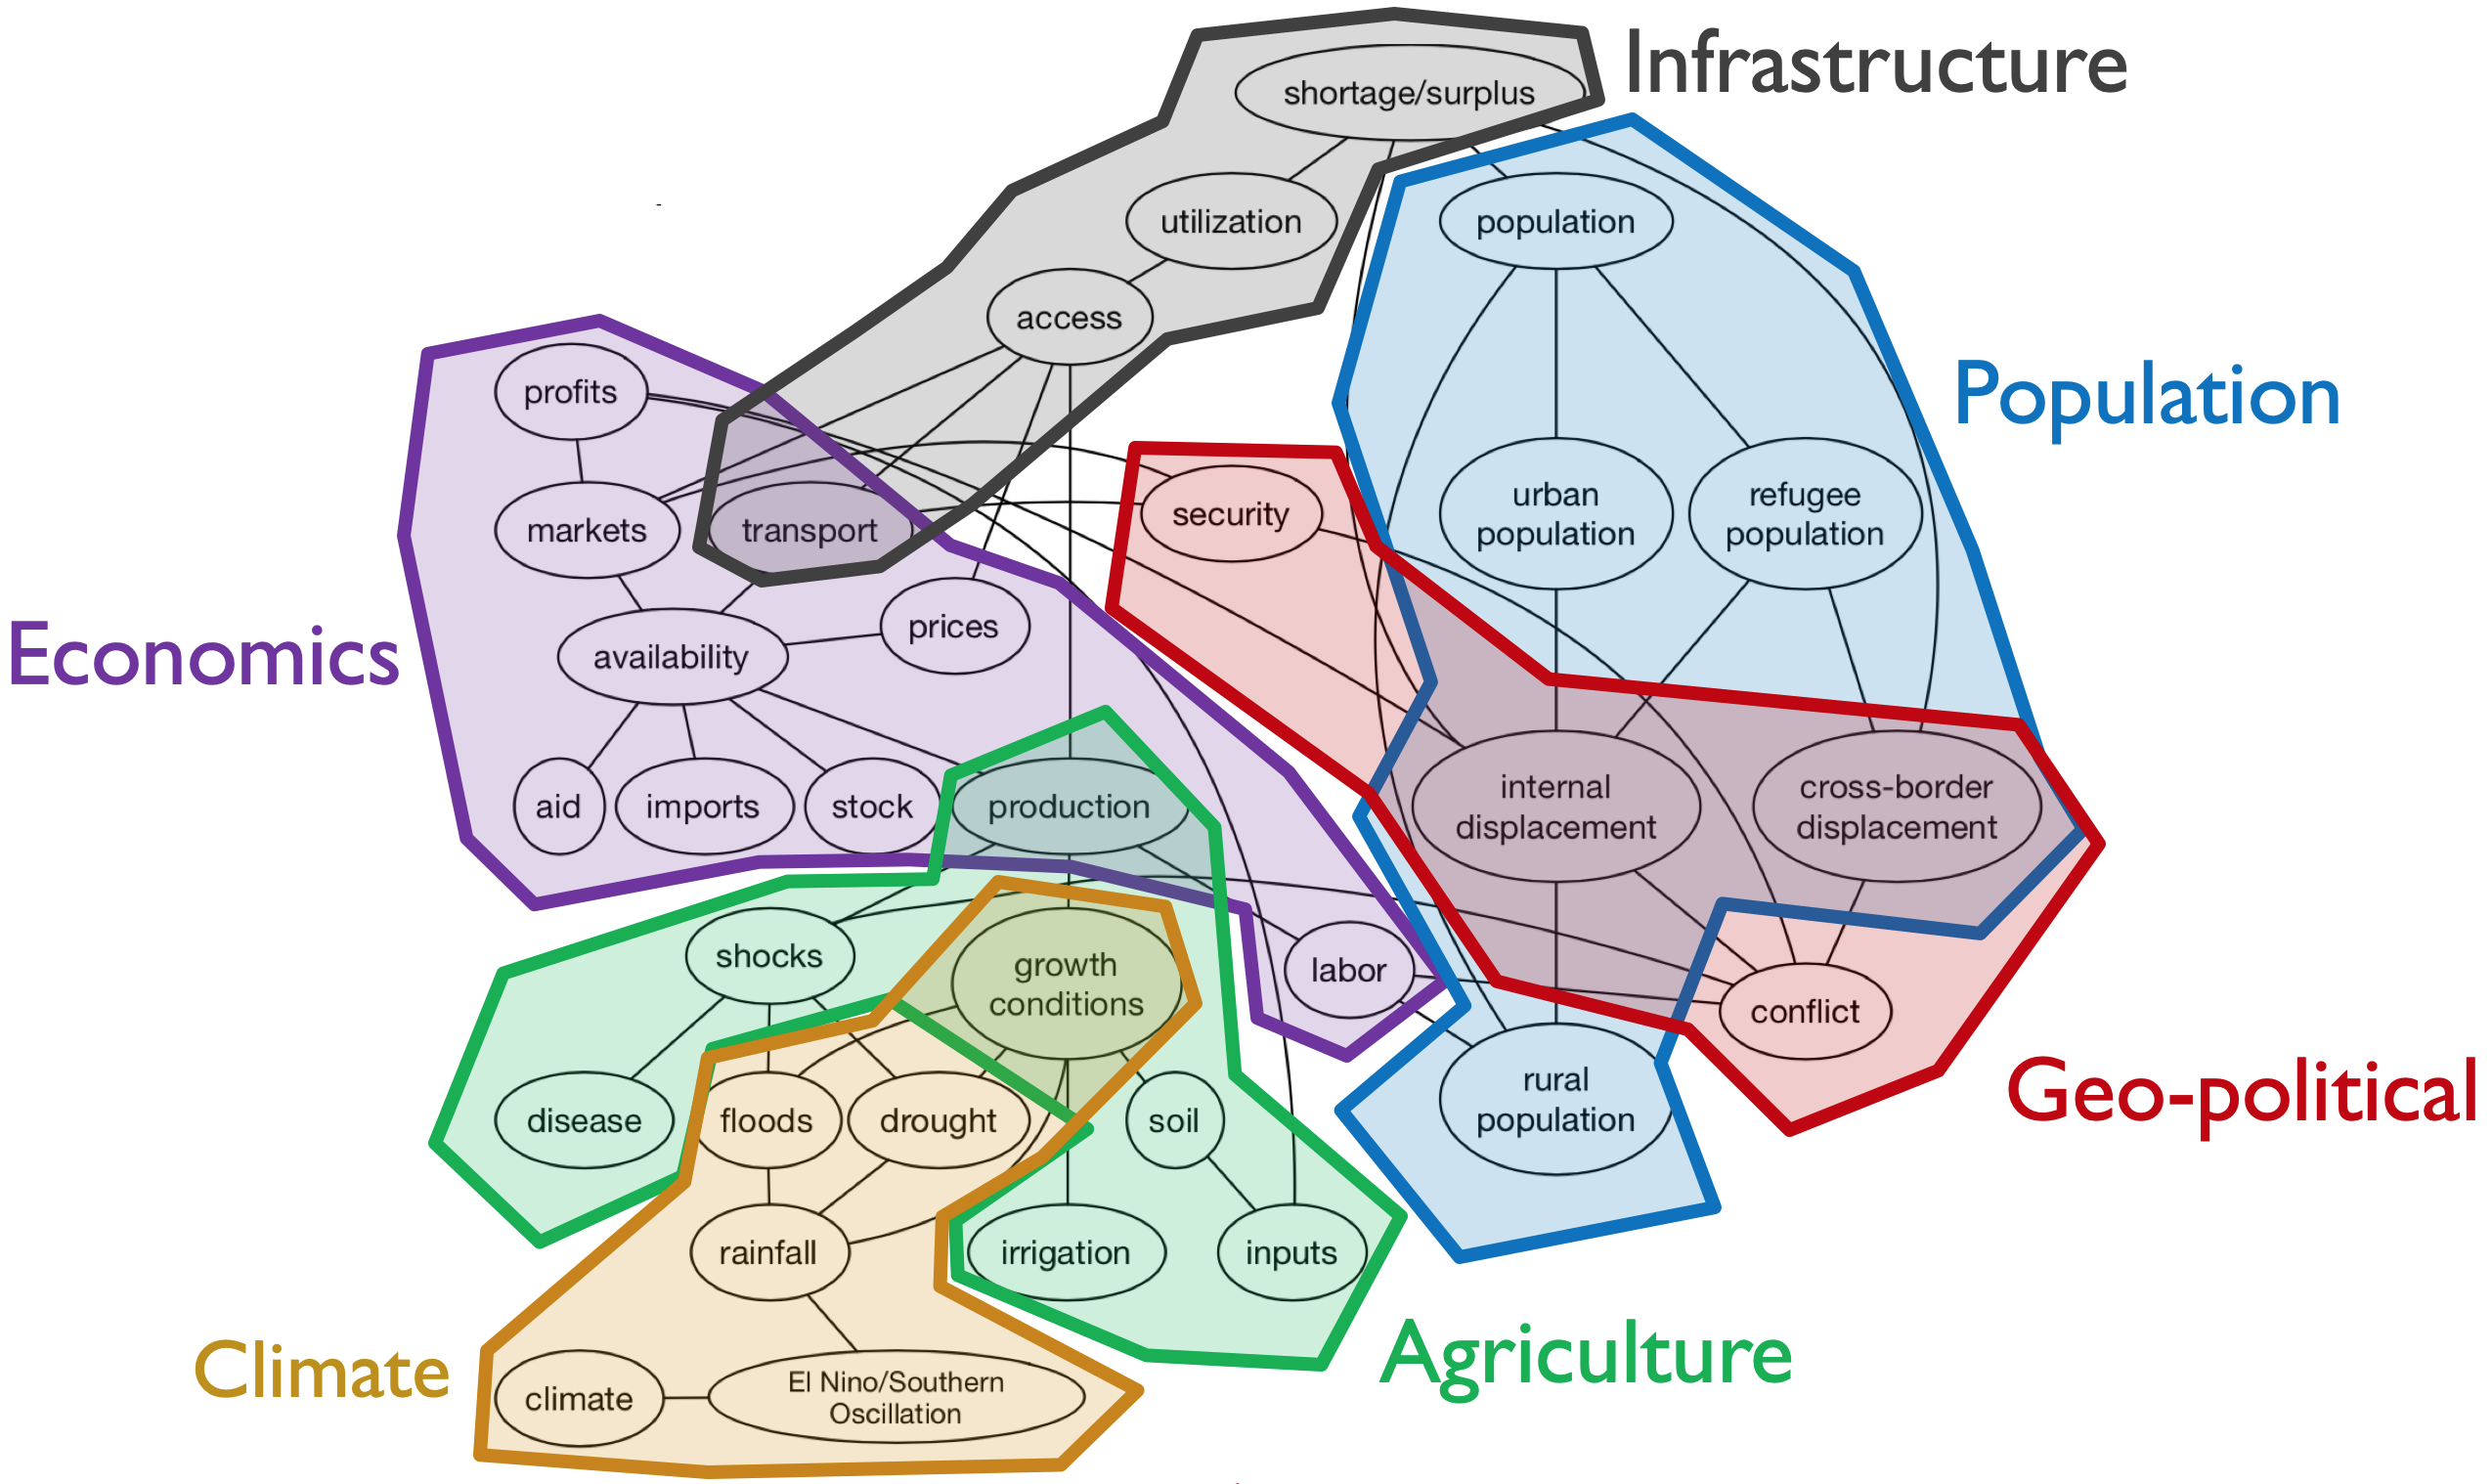
\includegraphics[width=\textwidth]{model-composition}
  \caption[Model Composition Web]{An illustration of how multiple scientific models from a diverse array of fields can be combined together to produce a meta-model of a much larger real-world system. In this meta-model each node represents a system that is modeled with a scientific model. Links between nodes correspond to connections between the separate models. Model composition is the process of determining which of these links are appropriate to make.}
  \label{fig:composition_example}
\end{figure}

Models can be composed when links can be identified between models.
These links are commonly in the form of shared model variables, where the output of one model may be the input of another, but more complex linkages can occur as well.
Sometimes a small structure of additional variables must be added in order to compose two models together.
This structure creation is an example of the task of \textit{model augmentation}, which is closely associated with the task of model composition since oftentimes augmentation is required before two models are able to be linked together.

Executable models are generally implemented in a wide range of different programming languages, using a variety of different programming paradigms, and also appear in a context of different conventions for documentation through publications and code comments. Engaging in any of the modeling tasks described above generally requires significant additional labor, such as defining a common model interface that allows for linking of variables, adapting model analysis techniques to specific code bases, or additional coding in a specific code base in order to implement model augmentations. These tasks also require direct involvement of a number of different kinds of expertise, including the domain modelers, model analysts, decision makers, and software engineers.

{\bf In this thesis, we propose a framework to help automate and augment significant portions of this process, in order to reduce the additional labor required to bring models together into a common representation.
In particular, we propose a set of methods for \textit{model extraction and assembly} that can identify and extract information about computation performed by the model from the source code into uniformly represented executable model framework.}

\section{Contributions\label{sec:contributions}}
The work presented in this thesis is a component of the larger AutoMATES\footnote{\url{https://ml4ai.github.io/automates/}} (Automated Model Assembly from Text, Equations, and Software) project \citep{pyarelal2019}, which is currently under way in the UofA School of Information ML4AI lab.
As the name suggests, the goal of the AutoMATES project is to assemble models from source code and documentation containing definitions of modeling domain concepts and equations that describe the relationships between variables.
To accomplish this goal, the AutoMATES project has three information extraction modules, focused on extracting information about models from the sources mentioned in the AutoMATES title.
The three extraction modules are the \textit{Text Reading} (TR) module, which extracts information about models from publications and other source texts, the \textit{Equation Reading} (ER) module, which extracts information from pictures of equations associated with models found in publications, and the \textit{Program Analysis} (PA) module, which extracts the functional wiring among variables to represent the computation expressed in source code as a dataflow model. The PA module currently focusses on extracting the dataflow model from Fortran, but this will be extended in the future to support program analysis of other languages as well.

This thesis presents a core contribution to the AutoMATES project, the \emph{Unified Model Assembly Framework} (UMAF).
As a component of the AutoMATES project, this framework plays the role of automatic assembly of models given the information extracted from the TR, ER, and PA modules.
UMAF integrates source code, text and equation information into a unified representation of a scientific model, called the \emph{Grounded Function Network} (GrFN), that is executable, comparable, and composable.
Combining these capabilities into a single framework provides a facility for domain-expert model developers and analysts to now analyze and compare models within a uniform framework, greatly simplifying model analysis tasks that to-date have required enormous manual effort.

UMAF does not take the human out of the loop: domain expertise and human guidance are still needed to identify variable value ranges of interest to a modeling application, as well as to identify supplement mistakes of omission and commission that may be made during variable grounding.
Ongoing and future development is also required to scale the methods to effectively handle larger model code bases.
UMAF is, to our knowledge, the first general approach to automating model extraction and assembly from source code to support model analysis, comparison, choice, and composition.
We also believe that UMAF provides a basis for a new kind of model curation and debugging, allowing one to compare changes within evolving code bases but from a modeling domain-semantics perspective
However, exploring use of UMAF for this purpose will be the subject of future work.

\section{Roadmap\label{sec:roadmap}}
This thesis is organized to present how UMAF is able to assemble models from information extraction from source code, text and equations, and then to show how to models created by UMAF can be used to aid modelers in analysis, model choice, and model composition.
During the course of this thesis we use two models from the Decision Support System for Agrotechnology Transfer (DSSAT)\footnote{\url{https://dssat.net/}} software system \citep{DSSAT} to illustrate the capabilities of UMAF and the associated analysis methods outlined in Section~\ref{sec:contributions}.
The source code used in this study is aimed at modeling the natural phenomena of Potential Evapotranspiration (PET).
The specific models we use are the Priestly-Taylor model of Potential Evapotranspiration (PETPT) and the ASCE model of Potential Evapotranspiration (PETASCE).

Chapter~\ref{chapter:related_work} reviews previous work that has been done in the areas of scientific model extraction, assembly, analysis, comparison, and composition.
Chapter~\ref{chapter:umaf} introduces the algorithms used to assemble models from source code into a form that is both executable and comparable across competing models by utilizing information from source texts to ground variables present in the models.
Finally, Chapter~\ref{chapter:conc_and_future} concludes with a discussion of the results and implications of UMAF and introduces possible extensions for continuing this research.

\chapter{MODEL EXTRACTION FROM SOURCE CODE\label{chapter:extraction}}
In order to perform analysis on scientific models found in software we must  extract that necessary associated source code and then represent the model in a form that supports model analysis and comparison within a programming language-agnostic framework.
The technique developed must be generalizable to allow model extraction from source code of the various programming languages that are used to define scientific models.
While large variations in syntax exist among the various programming languages used to encode scientific models, they can all be abstracted to a unifying abstract syntax tree (AST) representation \citep{aho1986dragonBook}.
Constructing an AST representation of a program requires a large number of design decisions that are largely dependent on the intended use-case of the information contained in the AST.
For the purposes of model selection we are keenly interested in identifying all potential models contained in the AST, as well as being able to easily inspect data-flow through the AST.

This chapter will begin with a discussion of the AST representation design decisions made to facilitate model extraction from source code.
Following this discussion will be an explanation on the conversion process from the AST representation of a model to an executable computation graph.
This chapter will conclude with an analysis of the computational cost of running the computation graph for a model and means of reducing this cost by leveraging vectorized computation and GPU computing resources.

At the time of writing this thesis, the \emph{program analysis} (PA) pipeline of the AutoMATES system supports analysis of source code from the Fortran programming language.
The AutoMATES project intends to eventually expand the scope of PA to support analysis of other widely used language and for the purposes of \emph{model analysis} (the focus of this thesis), the subtle language differences that will be introduced from different programming languages will be handled by the PA pipeline, before being represented in the intermediate AST form.

\section{Grounded Function Network Extraction\label{sec:grfn_extract}}
When translating a source code program, the SMS pipeline will receive a JSON specification and a set of associated lambda functions as input.
The JSON specification will fully represent the control-flow of variables through the original source code.
The lambda functions file will contain all of the individual computations necessary to execute a model that is faithful to the models found in the original source code.
From these two files the SMS pipeline will construct a scientific model that will be executable and can be used for comparison and analysis.

This executable model is called a Grounded Function Network (GrFN).
As the name suggests, this model will be a network.
A network is a directed acyclic graph that contains a set of source nodes and a set of sink nodes \citep{bondy1976graph}.
A node is considered a source node if the in-degree of the node, the number of directed edges arriving at the node, is zero.
Similarly a node is considered a sink node if the out-degree of the node, the number of directed edges leaving the node, is zero.
The name GrFN also implies that this network will be a network with functions.
Indeed this network will include two types of nodes, variable nodes and function nodes.
This network will be bipartite such that no function node has an edge incident to another function node, and no variable node has an edge incident to another variable node.
Since GrFN is intended to represent a scientific model, the source variable nodes of the GrFN will be the inputs of the model represented by the GrFN, and the sink node, which will be a variable node, will be the model output.
It is possible for the model to have some function nodes as sources to the network.
These represent literal assignment functions.

The last element of the GrFN name, \emph{grounding}, refers to how we interpret, and therefore potentially match during model analysis, the variable nodes of a model.
GrFNs must be comparable upon their variable nodes, since the variables track the actual observed and calculated values.
The assumption made here is that the software, as an instantiation of a scientific model, represents some aspects of the world, and the states of these modeled phenomena will be represented in the software by variables.
As defined in code, variables from two different models that represent the same phenomena could have different names, and two variables that represent different phenomena could have the same name.
In the AutoMATES project, the inference of what source code variables represent is a result of combining information from reading source code comments associated with source variables and other code documentation, along with text from associated scientific literature. Reading extracts and links mentions of domain concepts found in these sources. The result of this grounding process normalizes variable names so that, when successful, the GrFN representations of two different models about the same phenomena can be compared -- if two variables share the same name, they are assumed to be about the same aspect of the modeled domain. This inference process is not a focus of this thesis work; instead, we assume here that variable grounding inference has been performed and is represented by appropriated named variables within the GrFN representation, and instead develop the algorithms responsible for model analysis based on the grounded GrFN representation.

\section{Source Code to Computation Graph Example\label{sec:code_to_cg}}
To illustrate the process of constructing an executable computation graph from source code, consider the simple model for crop yield example from Figure~\ref{fig:simple_crop_CAG}.
The Fortran code for this model is shown in Figure~\ref{crop_code} below.
\FloatBarrier
\begin{figure}[!htbp]
    \label{crop_code}
    \centering
    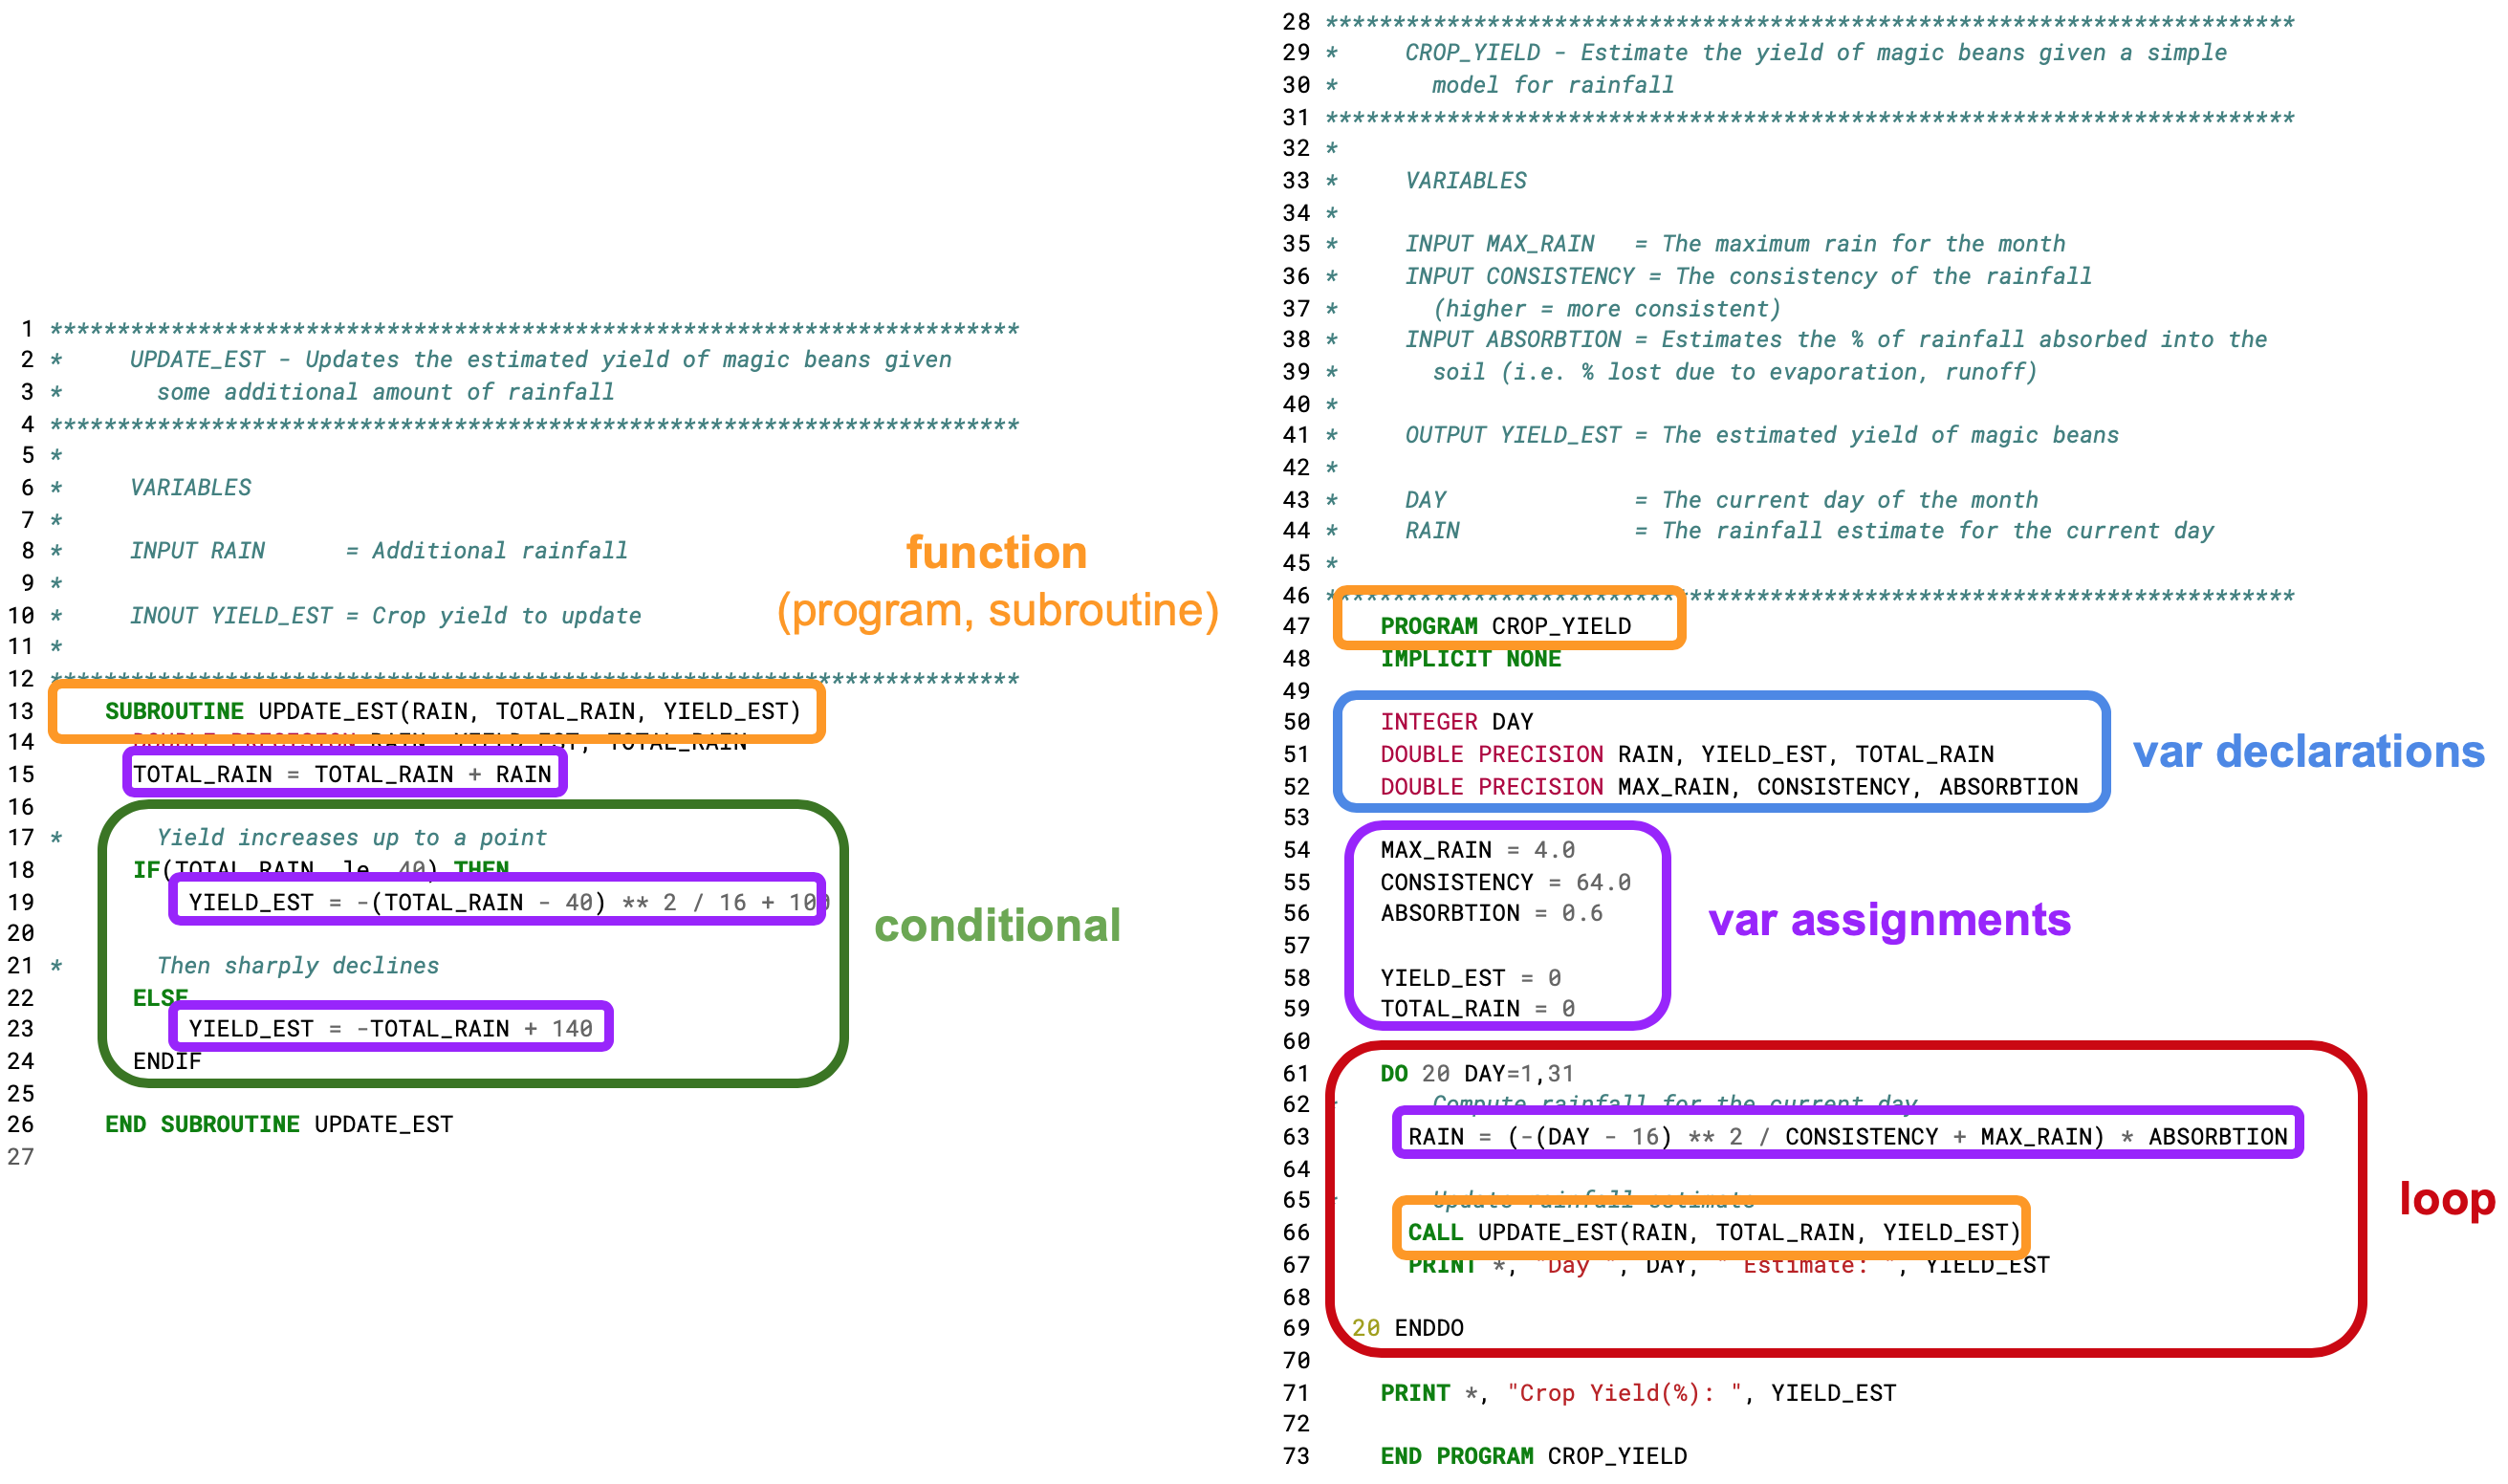
\includegraphics[width=\columnwidth]{CROP_YIELD_CODE}%
    \caption[Crop Yield Model Source Code]{Fortran source code for the simple model of Crop Yield.}
\end{figure}
\FloatBarrier

From inspecting the source code we see that this model has many programming idioms that need to be handled in order to create an executable computation graph for the source code.
As noted in the figure this includes subroutines, conditional statements, variable declarations, assignment statements, as well as loops.
The SMS pipeline handles all of these idioms and is able to produce the following executable computation graph, shown in Figure~\ref{crop_grfn_cg} below, that is faithful to the structure of the model found in the source code. In the following section I will delve into the specifics of how the SMS pipeline is able to create an executable computation graph from a source code representation.

\FloatBarrier
\begin{figure}[!htbp]
    \label{crop_grfn_cg}
    \centering
    \includegraphics[width=\columnwidth]{CROP_YIELD_GrFN}%
    \caption[Crop Yield Model GrFN CG]{Executable computation graph for the simple Crop Yield model.}
\end{figure}
\FloatBarrier

\section{Computation Graph Generation\label{sec:cg_gen}}
While the program analysis module is tasked with extracting ASTs from source code the SMS pipeline is responsible for transforming extracted ASTs into executable representations of the contained scientific models.
In order to make the representation of the scientific models comparable and analyzable the SMS pipeline also requires grounding information from the TR module that allows variables present in the code to be associated with real-world variables and phenomena.
The program analysis module outputs the control-flow found in the AST into a JSON specification, and in addition will output a python file that contains a set of lambda functions.
% \ctm{[PAUL: The following description gets a bit awkward: you're introducing a lot of technical jargon along with implementation details (JSON files). First help your reader to understand what GrFN is attempting to capture: what the variables are and how their states are determined as a function of other variables (i.e., functions); lambda functions are the representations of these functions that assign variable states as a function of other variables... THEN explain that this is represented in a JSON file format to permit flat-file representation; The GrFN JSON representation captures all of the information about the computation graph along with all text grounding information extracted by the text reading pipelines.]}
The lambda functions file represent specific computations that are done during the program.
This is a representation of the data-flow of the program, and will need to be encapsulated in the GrFN.
The JSON specification has an ordered set of statements that completely describe the control-flow of the original scientific model.
From these two items the SMS pipeline will create a GrFN Computation Graph (CG) that will be an executable representation of the scientific model contained in the original source code.
Below are examples of extracted GrFN CGs for the PETPT and PETASCE evapo-transpiration modules, derived from actual Fortran source code from the DSSAT code base, both of which are available in Appendix~\ref{appendix:a}.

\FloatBarrier
\begin{figure}[!tbp]
  \centering
  \subfloat[PETPT GrFN Computation Graph]{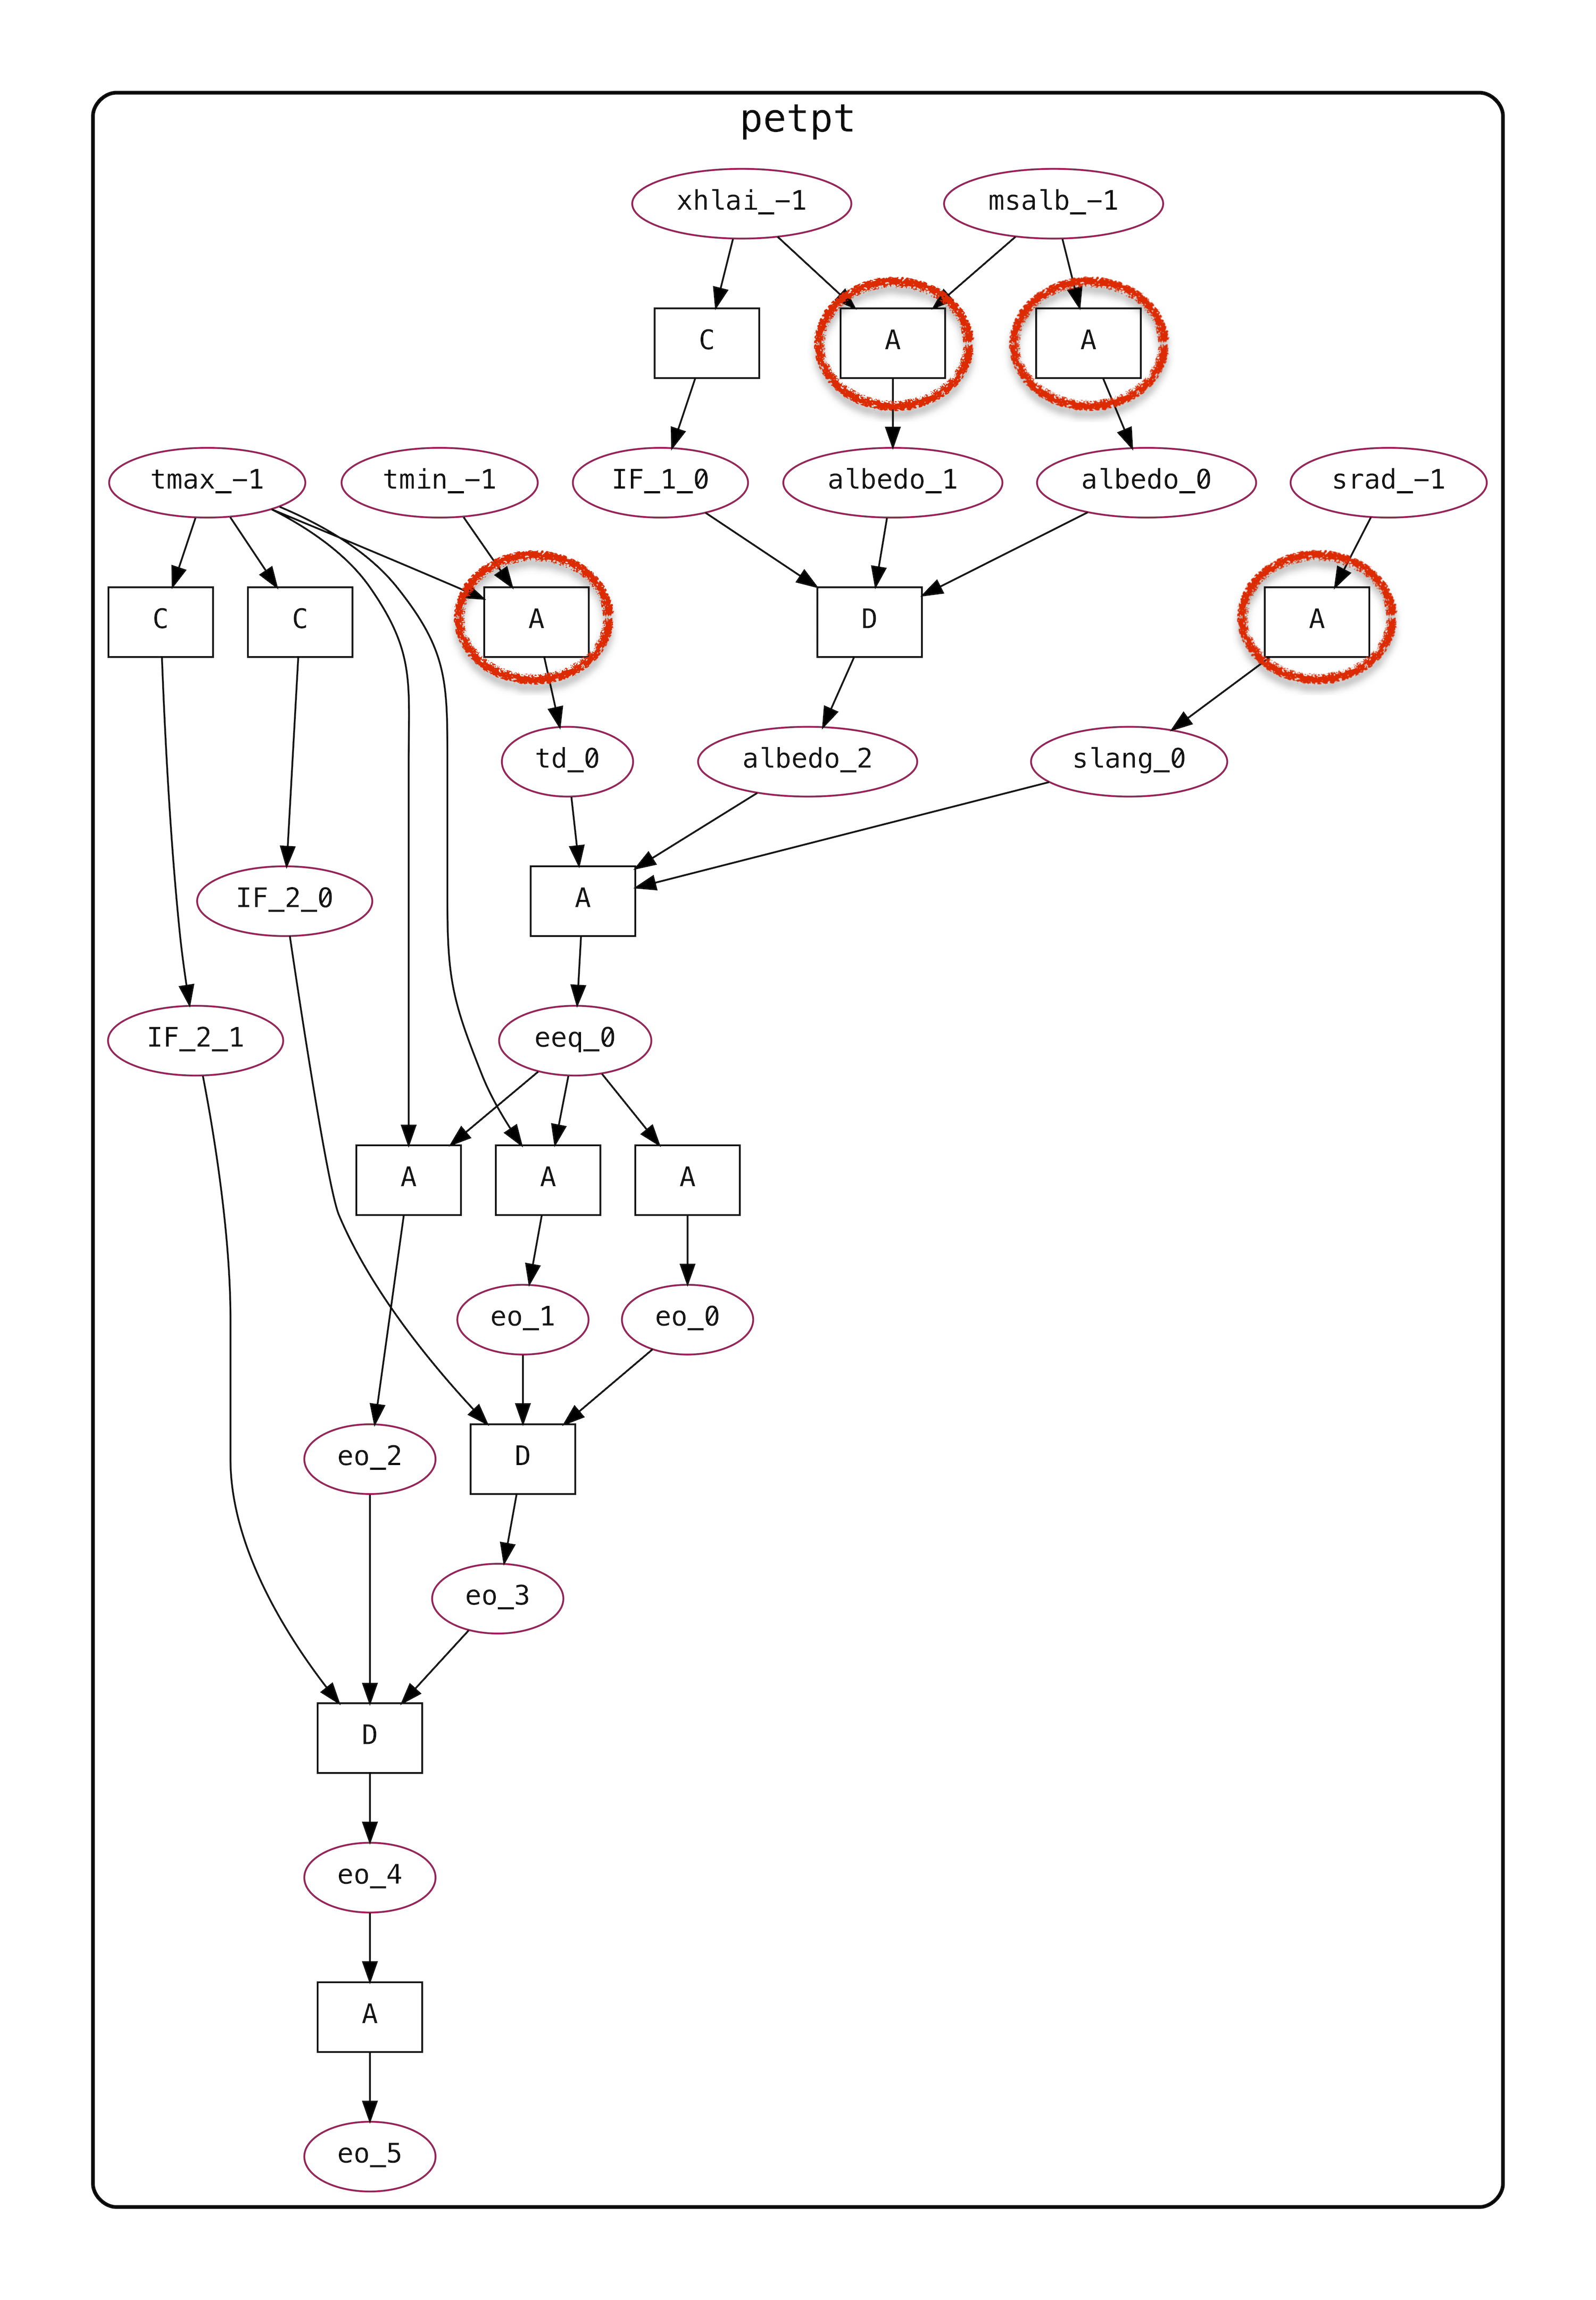
\includegraphics[width=0.45\textwidth]{PETPT_GrFN_smaller}\label{fig:petpt_grfn_cg}}
  \hfill
  \subfloat[PETASCE GrFN Computation Graph]{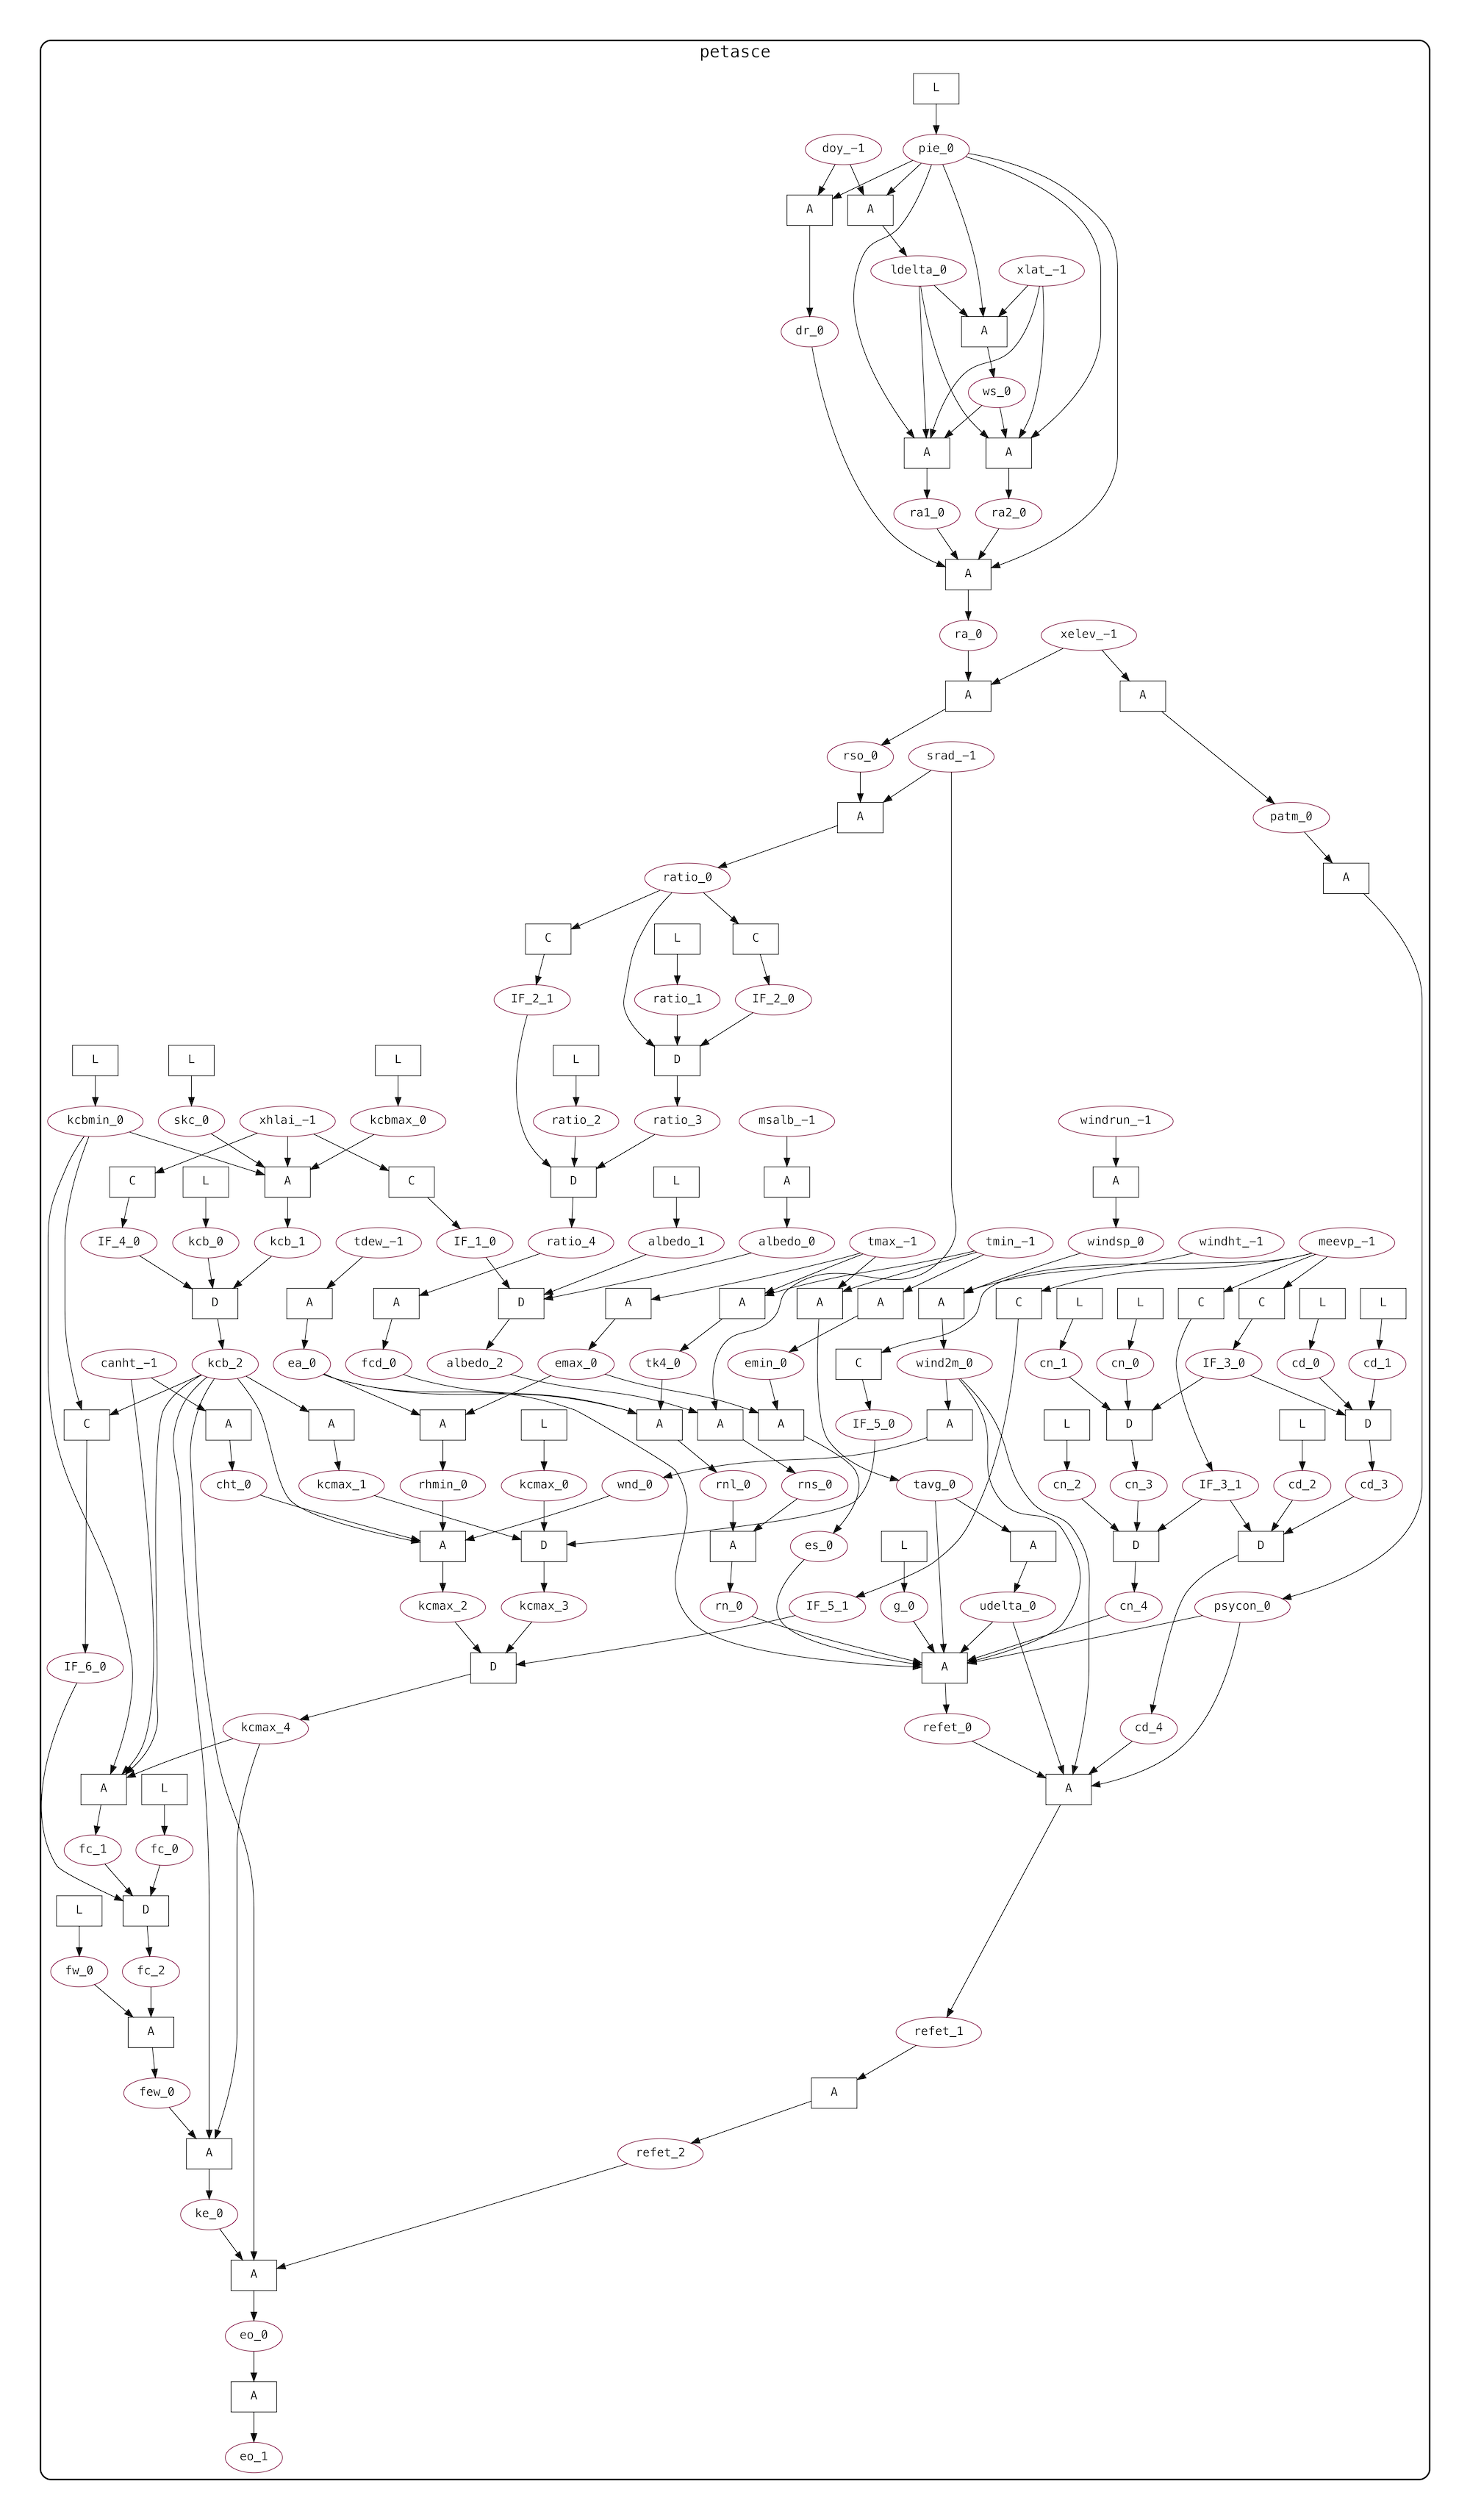
\includegraphics[width=0.45\textwidth]{PETASCE_GrFN_smaller}\label{fig:petasce_grfn_cg}}
  \caption[GrFN Computation Graph Examples]{Two examples of GrFN computation graphs (CGs). These CG representations include the variables, represented as circle nodes, with names derived from the names extracted in the source code and variable name grounding inference; the variable names also include a numeric index representing variable state changes during processing (see text for further details). Function nodes are depicted as squares with a single letter representing the type of function contained at the node. Function types include: assignment (A), conditional (C), decision (D), or literal (L). Note that in both CGs, the output nodes are variable nodes the inputs of the network can either be variable nodes or literal assignment function nodes.}
\end{figure}
\FloatBarrier

The first component of the SMS pipeline will be to develop the set of rules for how to traverse the JSON and handle the included statements to provide a clear view of how to construct a GrFN CG.
During GrFN CG construction, data-flow through the contained variables will be represented by creating function nodes that contain the computations described in the lambda functions file.
In the following subsections I will present the rules for generating the control-flow structure of a GrFN CG from the associated JSON specification.

\subsection{Containers and Function Calls\label{sec:containers}}
At the top level the JSON has a list of containers. These containers represent different scope levels in the source program. A container can be a function or subroutine found in the source code or a loop. The branches of a conditional will not be considered containers due to the nature of how the GrFN will be wired to deal with conditional evaluation. a container will contain a body that will be in the form of an ordered list of statements. These statements will correspond to statements from the original source code that was present in the container. Computation graph construction will begin at a top-level container and will process through the statements in the container, constructing the computation graph as it goes. When a statement that references a new container, such as a function call, is reached the body for that statement will be processed and connected to the computation graph that is being generated. Once this task is completed, the rest of the body for the original container will be processed. This recursive process works well for traversing all containers and constructing a computation graph based upon the statements contained in each container as long as no container has a call in it's body to another container that also has a call to the original container. Unfortunately this is precisely the case with recursive functions. They act as a special case for this processing pipeline and thus they are handled separately as will be discussed in subsequent sections.

Landing on a function call statement when parsing the body of a container is an indicator to begin processing the child container referenced by the function call, before proceeding with the rest of the statements in the current container.
The only difficulty in handling this call statement deals with the correct wiring of variable inputs into the child container.
To accomplish this task a set of live variables is tracked during the processing of the body for the current container.
As variables are updated they carry with them an index that denotes how many updates have occurred to the variable.
Variables that are inputs to a container start with an index of $-1$ and new variables defined in a container start with an index of $0$.
Once a new container statement is reached, the collection of live variables with their current indices is past into the new container.
This permits variables to be wired appropriately across containers.

\subsection{Assignment Statements\label{sec:assg_stmts}}
% \ctm{[PAUL: with a concrete example to ground this discussion, you can then point to a specific example in fortran code where an assignment is made...]}
During the processing of a container, when an assignment statement is reached it will include the following items:
\begin{itemize}
  \item A list of source variables
  \item The name of a lambda function
  \item A target variable node
\end{itemize}
Using these items the wiring for an assignment statement performs the following tasks to fully incorporate the information contained in the assignment statement into the GrFN CG:
\begin{itemize}
  \item Create a new function node for the lambda function
  \item Create a new variable node for target variable
  \item Create new variable nodes as needed for the input variables
  \item Create a directed edge from each input variable node to the function node
  \item Create a directed edge from the function node to the target variable node.
\end{itemize}
The computation required for an assignment statements can be handled by loading the assignment statement found in the source code into the function node generated during the wiring process of an assignment statement.
This allows values to propagate from the input variable nodes to the output variable node during GrFN CG execution.

\subsection{Conditional Statements\label{sec:cond_stmts}}
Conditional statements are handled via a set of two lambda evaluations.
The first evaluation is known as a \texttt{conditional} function node, that will actually evaluate the conditional property.
The second is a \texttt{decision} function node that takes as input the evaluation from the \texttt{condition} function as well as the two possible assignments for an output variable.
The \texttt{decision} function will be responsible for assigning the appropriate value to the output variable node based upon the conditional input.
Both the \texttt{decision} function node and the \texttt{conditional} function node output variable nodes as are artifacts that did not exist in the original source program.
Thus these will not be displayed when rendering the function node or variable node views of the computation graph.

\subsection{Indexed and Open-ended Loops\label{sec:loops}}
Loops naturally occur in source code as a means of expressing repetitive computations.
For the purposes of GrFN wiring, we want loops to be included, but we do not want to have backward links that would break the DAG property of a GrFN.
Therefore we will represent loops with plates that include an implicit edge back to the beginning of the loop that will be controlled by either an index or an exit condition. Therefore we will have two types of loops, the first being an indexed loop, and the second being an open-ended loop.
Indexed loops require a loop plate and have a specific index variable as well as a number of iterations through the loop.
They can easily be handled like containers as mentioned above, but require additional storage to handle information about the number of executions needed to satisfy the plate during computation.

Open ended loops will have conditional exit cases defined at a start or end point of a loop, which takes the form of an extra condition before looping or exiting the plate as compared to loops with an index and pre-defined amount of iterations.
An extra challenge is added when dealing with open-ended loops that can include multiple exit points (introduced either by \texttt{break} statements or \texttt{goto}s) as well conditional skip points where parts of the loop are skipped on an iteration (introduced either by \texttt{continue} statements or \texttt{goto}s).
This challenge will be solved by adding edges as necessary to the exit node for an open-ended loop to capture to capture the semantics of breaking and continuing.

% NOTE: section about loops from unstructured branching
In addition to explicit loops, programs can include two other forms of looping, namely \texttt{goto} statements and recursion.
In order to maximize the number of scientific models that can be expressed as GrFN the SMS pipeline will need to handle these inputs as well.
The usage of the \texttt{goto} statement has been hotly debated by computer scientists for nearly half a century.
In most modern programming languages the usage of \texttt{goto} or other such statements that allow for unstructured branching is prohibited.
However, the SMS pipeline will be used to extract models from source code inputs written in languages that do allow for unstructured branching, and thus this paradigm must be handled during the wiring phase of a GrFN computation graph.
The program analysis pipeline will handle detecting \texttt{goto}s and structuring the \texttt{goto} as an open-indexed loop.
Recursion is a commonly used software practice that must be handled for our computation graphs.
Most importantly, recursion must be identified and recursive edges that would create loops in the computation graph must be pruned.
Recursion can occur either as direct or indirect recursion.
In the case of indirect recursion a series of functions forms a loop that will repeat until a base condition is satisfied.
Identifying recursion is a task that will be handled by the program analysis pipeline.
Once a recursion loop is discovered, it will be handled the same as an open-indexed loop.
Once a \texttt{goto} or recursion loop is transformed into an open-indexed loop the SMS pipeline will handle adding it as a loop-plate to the overall computation graph in the same fashion as any other loop plate.


\section{Data Type Assignment\label{sec:data_types}}
So far I have discussed the wiring needed to create the computation graph that will allow a GrFN to be executed, and I have shown the methods necessary to make the GrFN executable. However, one more crucial component for creating a GrFN that we can perform inference upon is a discussion of how we will handle the actual data being processed from the GrFN. At the time of writing this thesis only basic data types are allowable in a GrFN. This includes numerical, string, and boolean values. These primitive data types are all singular values that represent a single phenomena, thus they match perfectly with the definition of variable nodes in the GrFN CG. The specification for each variable in a GrFN CG contains a type annotation that declares the data type of the variable. These values are derived from the JSON specification during the wiring stage of the GrFN. At execution time, these type annotations are used to validate a set of inputs and ensure proper storage format of computed variable values.

The infrastructure to represent complex data types such as Arrays, user-defined types, and unions in the AST form is still being developed by the program analysis team, and thus they will not be included in this thesis. The main challenge with representing these data types is that they are not singular variables, but are instead collections of variables. To properly perform inference over a GrFN CG all variable nodes must be singular variables, thus we cannot allow any of the above collections of variables to be represented by a variable node. This presents a problem of representation that will be studied  and resolved in future work that extends this thesis.

\section{GrFNs are Dynamic Bayes Nets\label{sec:grfn_as_dbn}}
Once we have extracted a GrFN CG that represents a scientific model we will want to analyze the model and compare it to other existing models.
Both of these tasks require us to be able to perform inference on the GrFN CG by observing the behavior of the model over a distribution of inputs.
A well defined methodology for performing inference over DAGs is to establish the DAG as a bayesian network \citep{bishop2006pattern}, a type of probabilistic graphical model, and then to use the robust set of methods associated with bayes nets to solve inference problems.
In this section I will now demonstrate how a GrFN CG is a bayesian network in order to unlock the use of inference on GrFN CGs.

A GrFN CG has a set of input variables that are wired as a network to the outputs of the model represented by the GrFN CG.
The inputs of the GrFN CG can be assigned values and will then return an output value for each of the GrFN CG outputs.
Recall that all variables in a GrFN CG are treated as random variables.
Bayes nets have a set of variables that are linked to observable random variables that exist in the real world.
This presents a challenge for representing a GrFN CG as a bayes net because several variables in a GrFN CG represent the same natural phenomena.
However, we can view a GrFN CG as a \emph{Causal Analysis Graph} (CAG) that allows us to visualize only the variable relationships present in the GrFN.
Below are the CAG views for the two GrFN CGs under study in this thesis. Notice that inspecting this view gives us a graph structure that looks similar to a bayes network that has loops (i.e. one that can be unrolled over time).

\FloatBarrier
\begin{figure}[!tbp]
  \centering
  \subfloat[PETPT GrFN CAG]{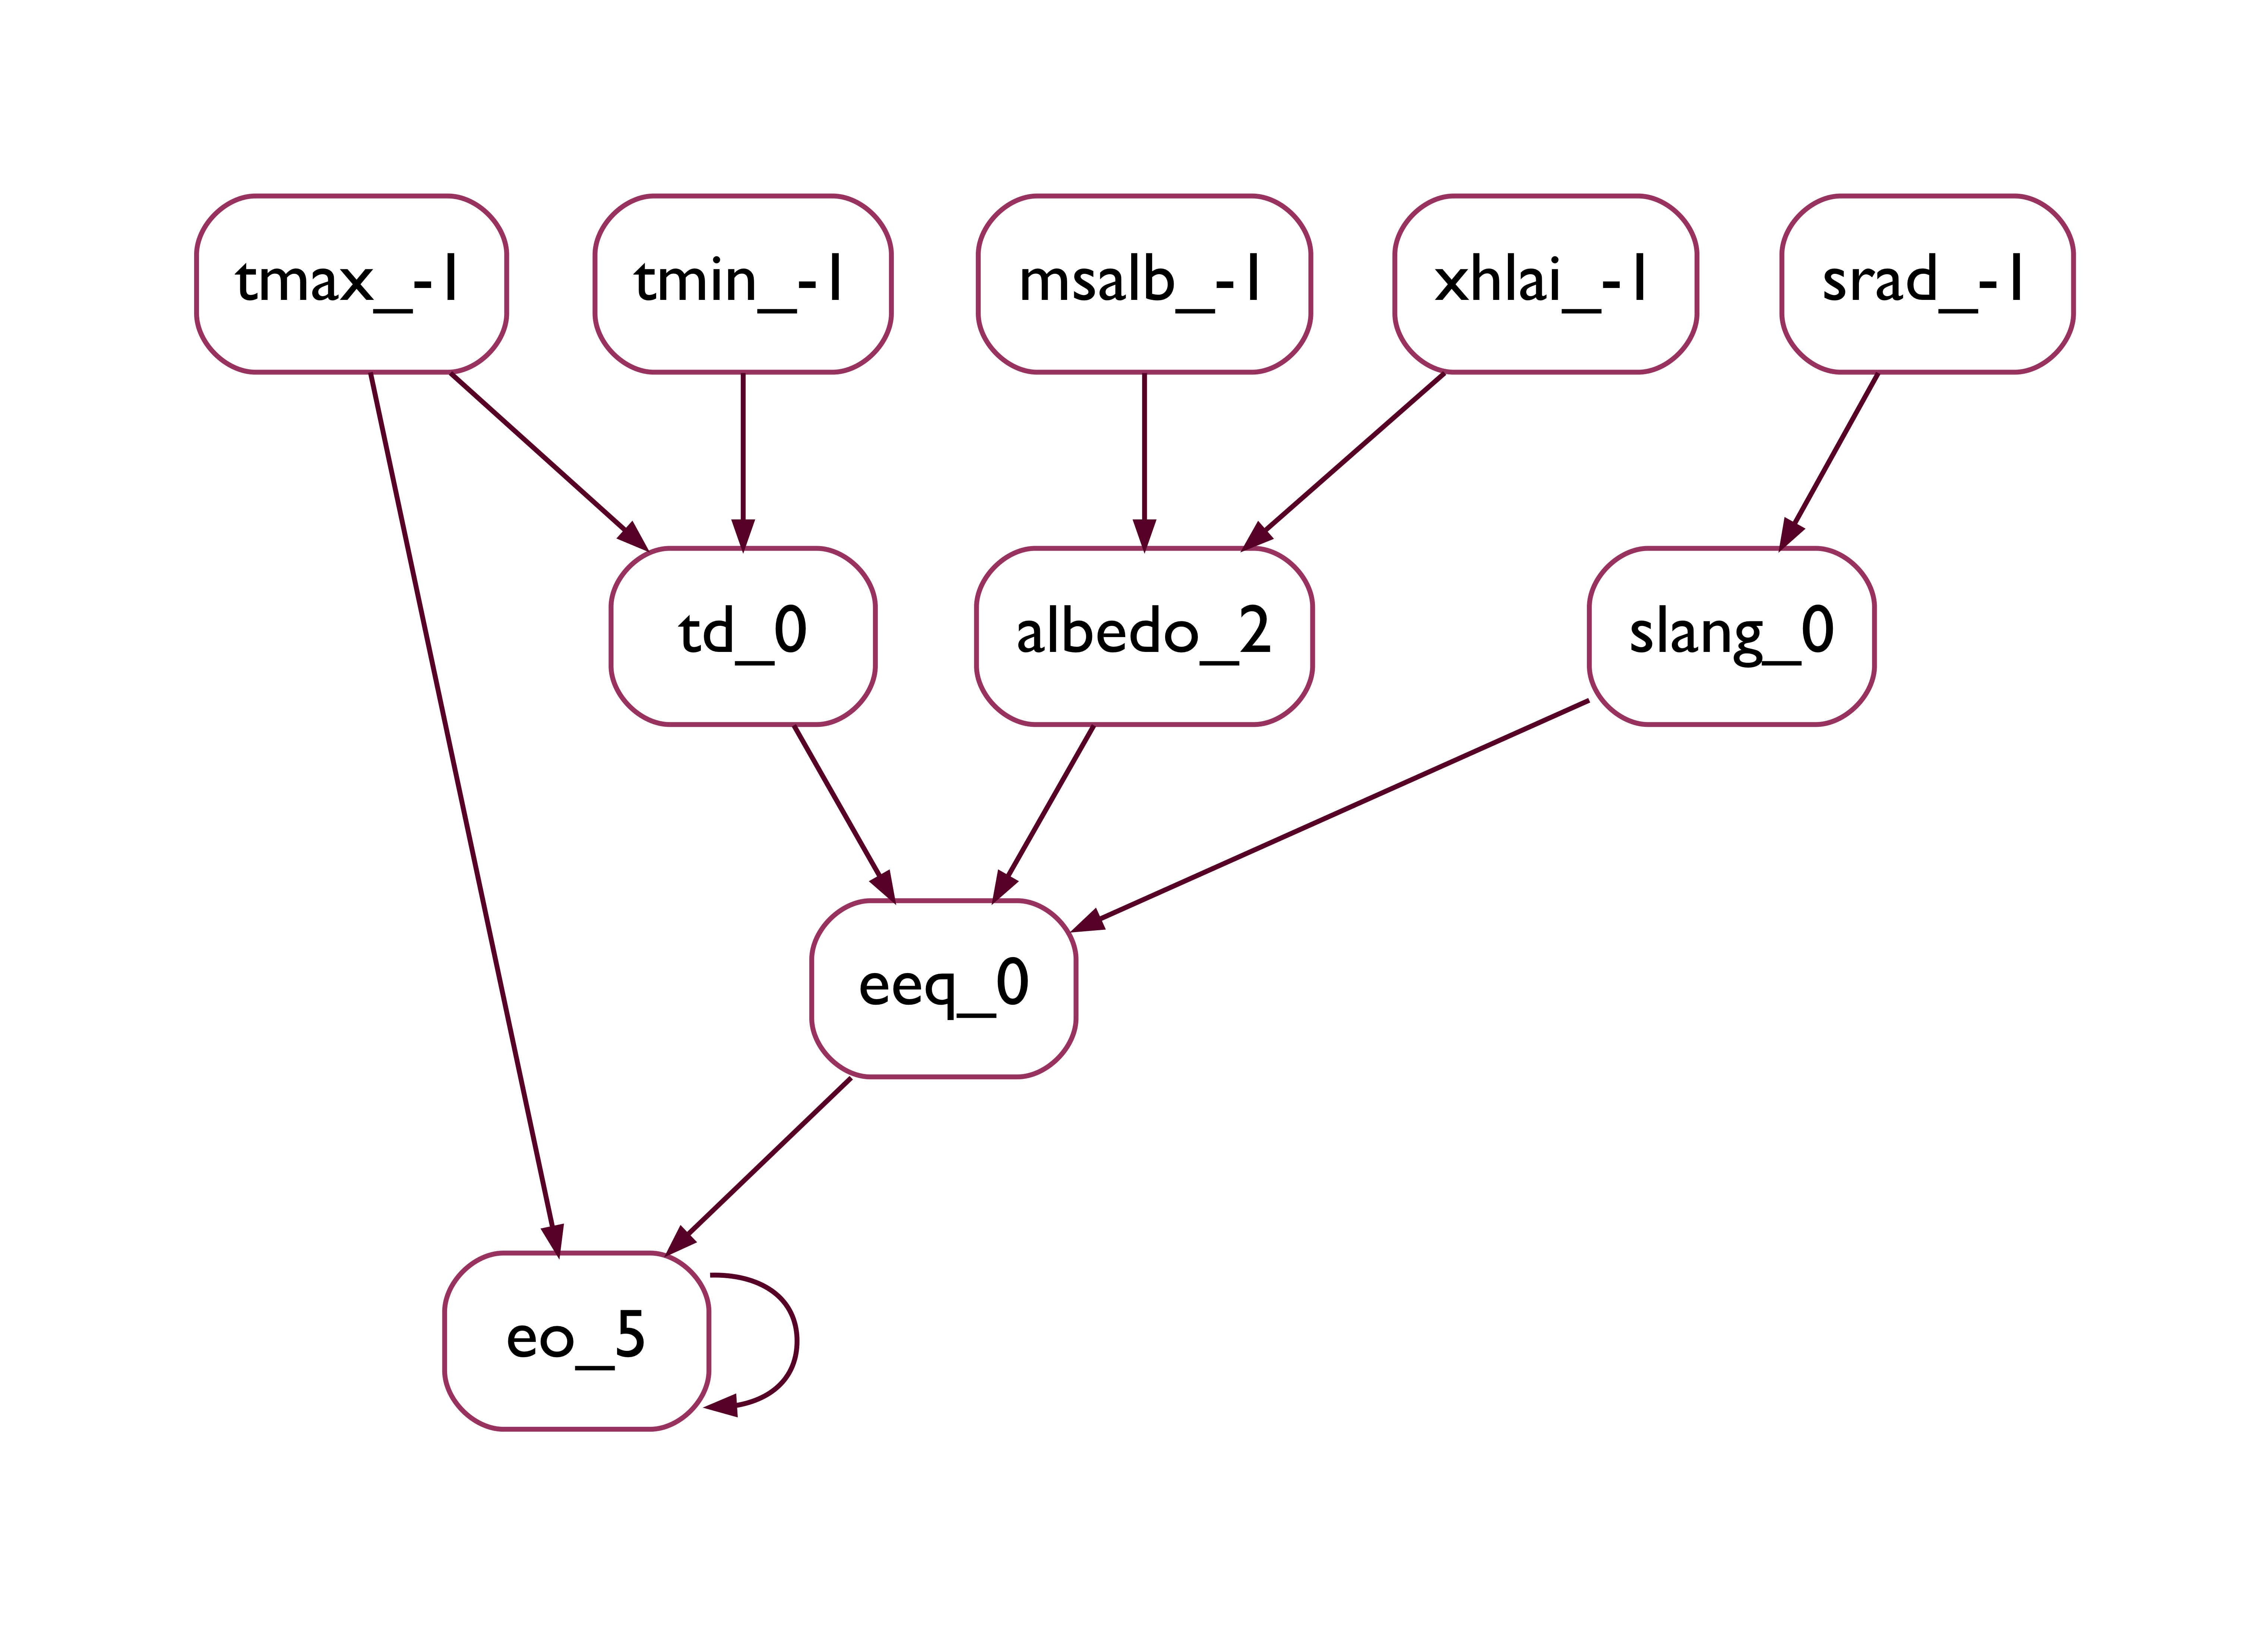
\includegraphics[width=0.75\textwidth]{PETPT_GrFN_CAG}\label{fig:petpt_cag}}

  \subfloat[PETASCE GrFN CAG]{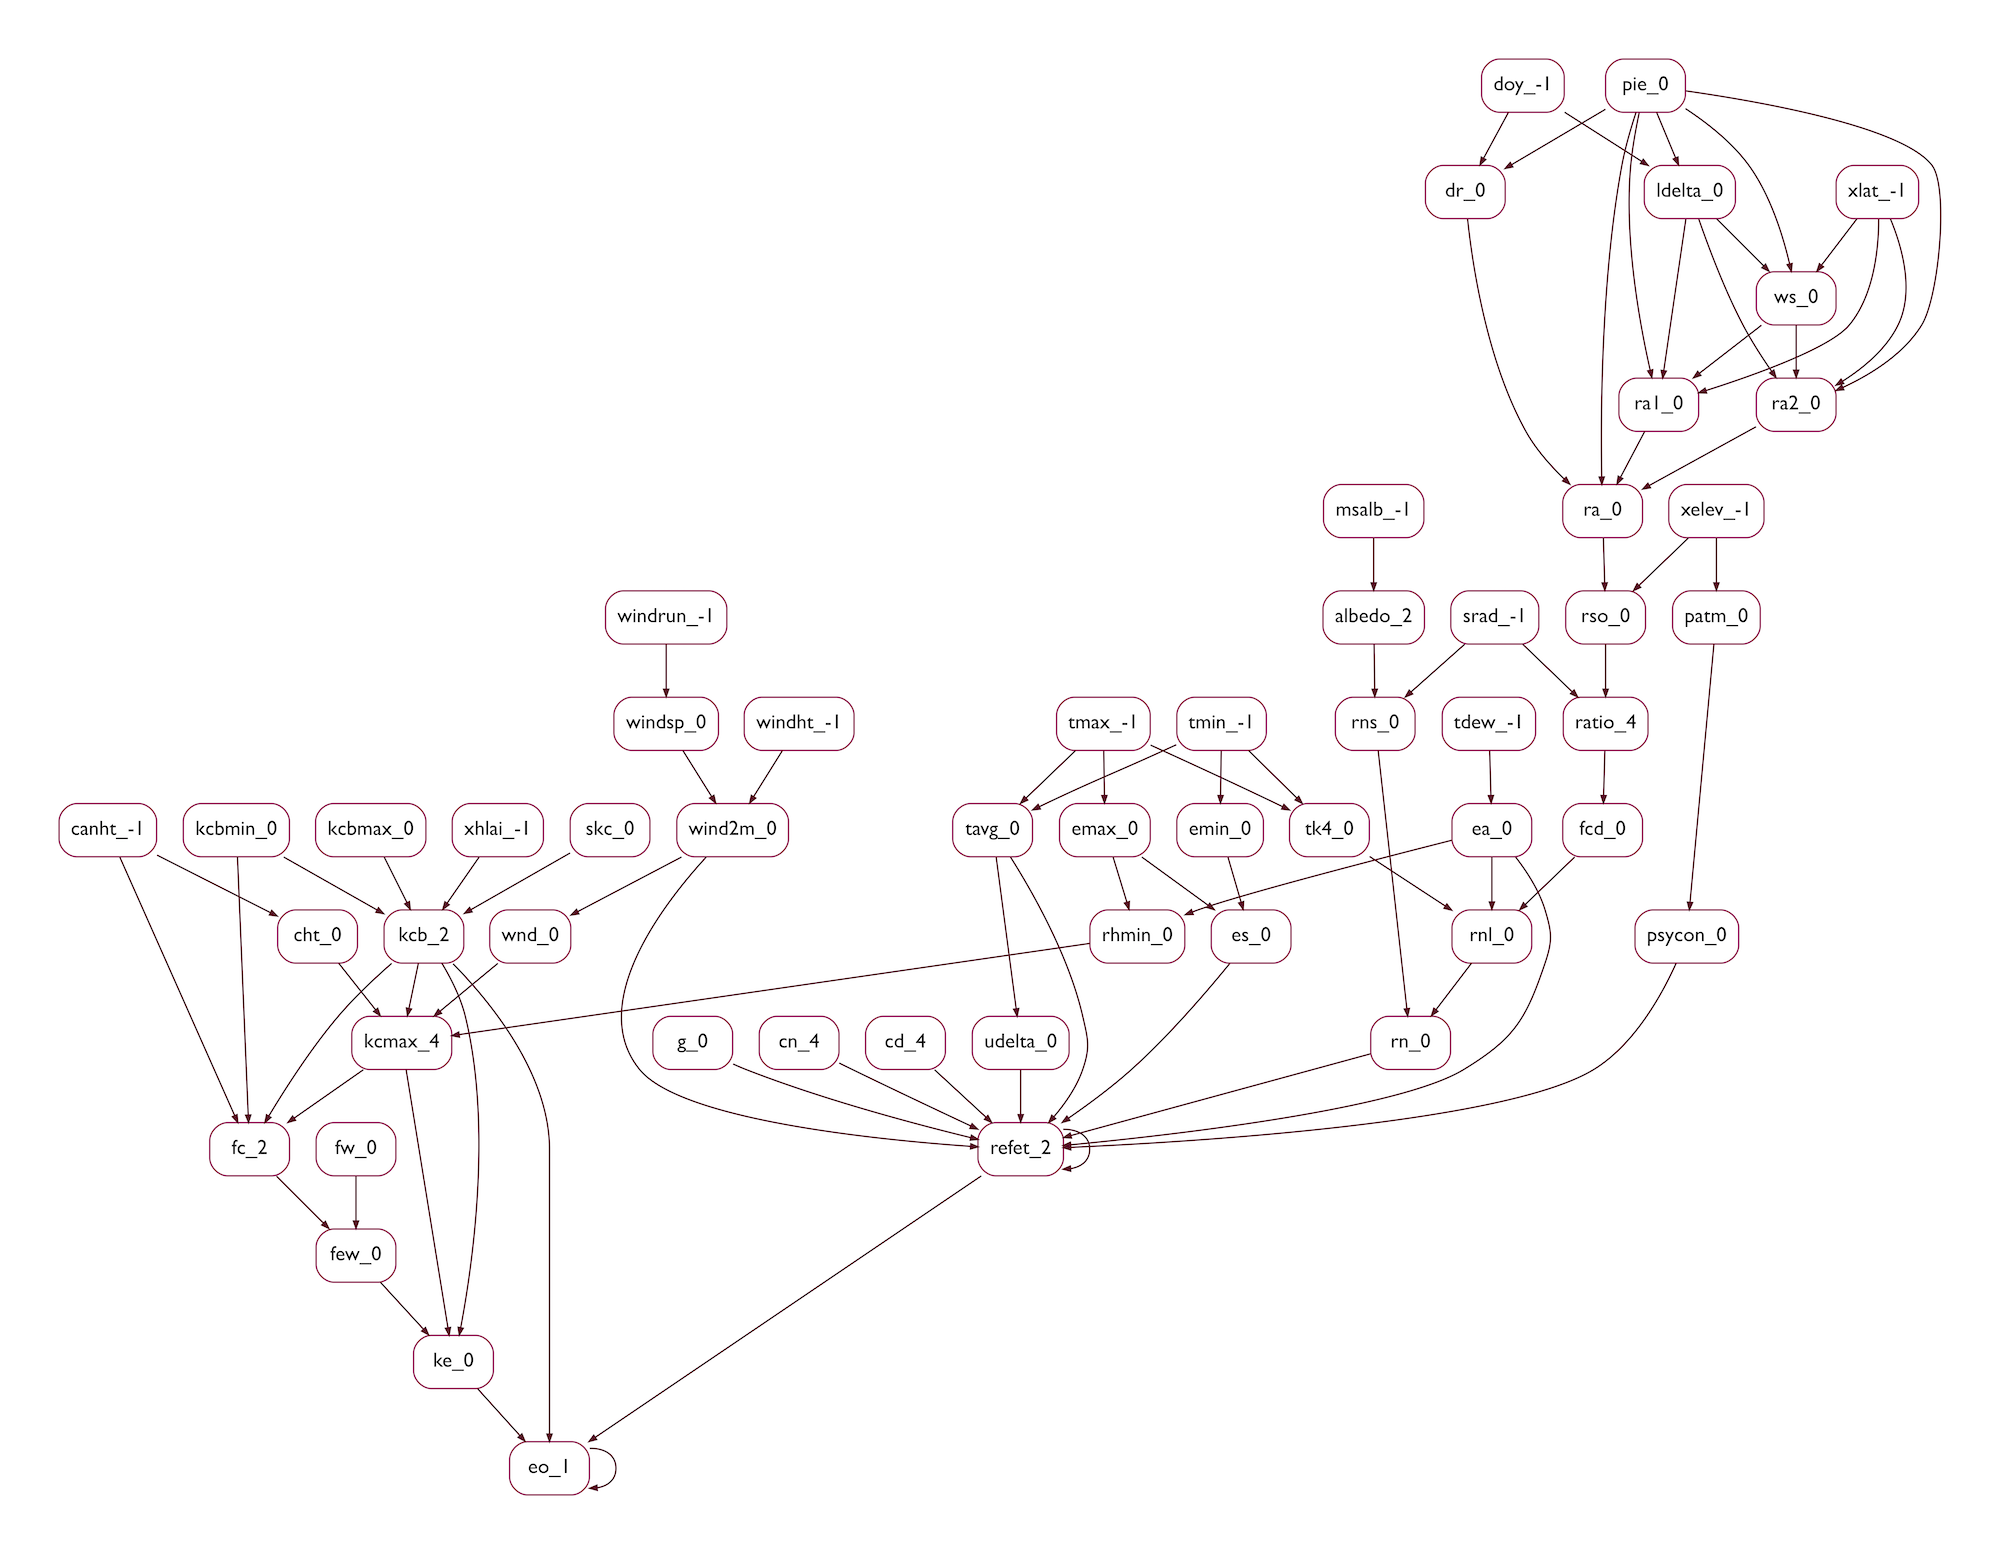
\includegraphics[width=0.75\textwidth]{PETASCE_GrFN_CAG_smaller}\label{fig:petasce_cag}}
  \caption[GrFN Causal Analysis Graph Examples]{Causal analysis graph views of the PETPT and PETASCE evapo-transpiration models.}
\end{figure}
\FloatBarrier

When treating the input variables as random variables we can induce a distribution over the values that they can take.
This distribution will then permeate through the function nodes to the other variable nodes in the GrFN CG.
For the GrFN CG to be a Dynamic Bayes Net (DBN) we need the probability distribution of the output variable to be a product of all of the input probability distributions \citep{pearl2009causality}.
During the computation of any inner variable in a GrFN CG we have a lambda function that denotes how the the inputs to the computation are to be combined to form the output.
All possible combinations are mathematical functions, that are able to be applied over the probability distribution of the inputs.
Therefore the resulting computed inner variable has a distribution that is the combination of the distributions over the inputs.
However, this distribution is not yet a probability distribution.
In order to create a probability distribution a normalization step is required so that the total probability mass sums to 1.
Once this step is complete we can see that we have satisfied the requirements for a DBN for the trivial case of a single computed node with a set of input nodes.
Since we are free to induce distributions on the input nodes of a GrFN, and all inner nodes and output nodes of a GrFN are defined in the same manner as the case explored above we can conclude that a GrFN CG is indeed a DBN.

\section{GrFN Computation Graph Execution\label{sec:cg_execution}}
Once the wiring stage for a GrFN has been completed, the GrFN CG must be made executable. The execution of a GrFN CG requires the execution of all functions stored at the function nodes of the computation graph. Therefore the problem of executing a GrFN CG can be simplified to the problem of determining an ordering of execution of the function nodes that allows for all of the function nodes to be executed without any failures. Of course a GrFN CG also needs to save the state of variables during execution in a way that allows the function nodes to access the information stored for each variable they require. In this section I will present the methods developed for the GrFN CG to handle the function evaluation ordering problem and the variable storage access problem.

\subsection{Call Stack Creation\label{sec:call_stack}}
Creating a computation graph from a GrFN specification allows us to formally represent an extracted scientific model as a graph data structure.
However, if we wish to analyze the extracted model, then we will need the ability to compute information over this data structure.
To accomplish this we introduce the idea of execution over a computation graph. The computation graph contains a set of function nodes.
Computing the lambda function stored at each function node is analogous to executing the computation graph from the set of inputs to the output.
However, the function nodes rely upon having values populated at each of their input variable nodes in order to perform their computation.
Therefore the task of executing a GrFN CG can be rephrased as determining how to order and execute the functions nodes contained in the computation graph.

A Naïve first-pass solution to accomplish this goal would be to use a graph traversal from the output to the inputs where at each function node, the node will determine whether values for each input variable node have been populated.
For any input variable nodes that have not been populated, the function node will call the parent function node responsible for computing the value of the input variable node.
Once all such calls have returned, the function itself will evaluate. This recursive calling procedure is very similar to message-passing, a method for inference on factor graphs.
While this will ensure correct model execution, this method of handling execution is not as efficient as possible.
To start the recursive call structure adds additional function setup and calls to the execution, on the order of the number of functions included in the computation graph.
The second obvious inefficiency with this execution is that the recursive operations must be done for each execution, and they require all function nodes to be executed sequentially.

These two concerns can be addressed by creating a call stack comprised of all the function nodes contained in the GrFN CG.
The order of computation between function nodes implies that the call stack is equivalent to a partially ordered set (poset) upon the function nodes \citep{simovici2008miningTools}.
Once this poset is recovered, execution of the GrFN CG can occur by executing all functions at the first level in the poset, then moving to the next level in the poset, and then repeating the sequence until reaching the end of the call stack.
This allows all function nodes at the same level in the poset to be executed concurrently, and the computation required to create this call stack only needs to occur once.

Computing the call stack requires a series of separate computations.
First a control flow graph (CFG) \citep{allen1970CFG} must be extracted from the GrFN CG.
As defined above, the GrFN CG is bipartite with respect to the variable and function nodes, such that no variable node is adjacent to another variable node and vice-versa for a function node \citep{bondy1976graph}.
Therefore a GrFN CFG can be extracted from the GrFN CG by simply squashing any variable node between a pair of function nodes into a singular edge connecting the two function nodes.
Since the GrFN CFG is derived from the GrFN CG it will have a set of input nodes.
Starting from this set of input nodes an index is assigned to each node, beginning at zero.
Each time an edge is traversed the index increases.
If a function node is reached and it already has an index the index is updated to the maximum of the current index and the newly calculated index.
Once the full graph traversal is complete we have an index for the poset.
Function node sets are created according to the index values, and the index values also provide the ordering of the function node sets.
Smaller index values correspond to the function node sets that are to be computed first.
Function sets can then be placed into the call stack by pushing the sets with the largest index value onto the stack first.
The GrFN CG now has access to a call stack that can be used to execute an input set.
During execution, when the call stack is being used, it can be maintained by pushing popped values from the stack onto a different empty stack.
After execution, the values can be popped from the temporary stack and pushed back on to the original call stack. This ensures that the call stack order will be maintained for the next execution.

\subsection{Computation Graph Input Execution\label{sec:input_execution}}
During execution, a GrFN utilizes a value storage tag at each variable node.
During computation, function nodes pull their input data from the value tag of each parent variable node of the function node.
The output from the function node is stored in the value tag of the variable node that is the child of the function node.
Function nodes are guaranteed to have access to the variable node input data at the time of their execution by the call stack execution order discussed in the previous section.
After all function nodes have been executed the output variable node of the GrFN CG will have the computed output value stored in its value tag.

While a GrFN CG is perfectly capable of executing one set of inputs at a time, as described in the method above, the CG can also handle executing over multiple sets of inputs at once.
The SMS pipeline accomplishes this by making use of the PyTorch tensor computation framework.
It is advantageous to compute multiple inputs at once using vectorized computations because pooling like computations lowers overall compute time.

\section{Model Overlap Identification\label{sec:overlap_identification}}

While analytical methods can provide a large amount of useful information to modelers about a single model, the real benefit of the AutoMATES system comes from the ability to automate comparisons among competing models. Competing models can be identified from the output variables of their computation graphs. After identifying a selection of competing models the comparison phase can begin.

For any two competing models of the same phenomena the comparison phase consists of the following:

\begin{enumerate}
  \item Identify the overlap between the variables in each models computation graphs. This corresponds to overlap in observable real-world phenomena.
  \item Extract the sub computation graphs for each model based on the variable node overlap.
  \item Perform analysis on the overlapping computation graphs and compare the results with the analysis results from the models whole computation graphs.
\end{enumerate}

In order to accomplish the tasks outlined above, I will introduce a new construct, known as a Forward Influence Blanket (FIB). A FIB is a specific instance of a Markov blanket \citep{pearl2009causality}, derived from a GrFN computation graph, that can be used for forward analysis.  % TODO: possibly define forward analysis and markov blanket
After the completion of these tasks the information gained from the comparative study of these models can be added to the final model report, or used for automatic model selection. In this chapter I discuss model comparison in terms of two models compared directly with one another. At the end of the chapter I will elucidate on the necessary steps to generalize this form of binary model comparison to a set of $N$ models.

\subsection{Identifying a Forward Influence Blanket\label{sec:fib_creation}}
Imagine the structure of two computational models of the same phenomena in the most general sense. We can say with certainty that both models will have the same output variable, namely the variable that represents the phenomena of interest. From this there are three options for how the set of input variables between the two computational graphs can overlap. The least interesting option is that the two models could share no inputs variables. This would mean that the computations involved in each model are wholly independent and could be combined if necessary in a trivial manner, at least at the input level. The more interesting option is that a subset of the inputs are shared between the two models. This entails that the models will make use of the same data, though the computations used to transform that data into a model output will almost certainly differ. It is possible that the set of input variables will overlap exactly between the two models; however, it is much more likely that there will be some input variables that are not contained in both. In the following subsections I will discuss how to build a computation graph that represents the computation present in a GrFN that corresponds to utilization of shared variable nodes with another model.

% TODO: Add material about Shared Structure Identification here
The shared structure components of a FIB for two models of the same phenomena are identified using the following strategy.
By definition the models share the same output variable node.
Therefore any shared structure will be within the range of a shared variable node, either an input variable or an inner variable node, and all the full computation path to the output node.
A set of shared nodes between the two graphs can be discovered using node name matching on the grounded node names.
This is done upon the CAG view of the GrFN CG so that variable nodes are only matched once and not once per update recorded in the overall CG.
Using the set of shared nodes and the output node we can discover all computation paths that lead to the output node by doing an exhaustive path search from each shared node to the output node \citep{sedgewick2002algorithmsInC}.
Combining the outputs from all of these paths together gives us the shared portions of each GrFN CG that serve as the basis for each models FIB.

% TODO: The section discusses Cover Set Variables
The key aspect of a FIB that distinguishes it from a GrFN computation graph is that the portions of the original computation graph that are not shared between the two models under comparison are pruned.
In order to ensure that the resulting models are still executable, variable nodes representing new inputs to the FIB computation graph must be retained.
This set of variables has been identified as the cover set.
Forming this cover set and adding it to the shared overlap portion of each GrFN CG as mentioned above is the last step necessary to fully create the FIB for each model.
Identifying a variable as being a member of the cover set stems from the initial shared graph structure extracted from the original GrFN CGs.
All nodes along the shared structure must be compared to the node structure in the original CG.
If any nodes are missing a branch that is present in the original CG then the immediate parent of the node must be added to the set of cover nodes and is grafted on to the FIB.
Once the set of cover nodes are added to the shared graph structure the FIBs for each model are complete.
To visualize what a FIB looks like for both a small and large CG we have added the FIBs that denote the overlap between the two evapo-transpiration models.

\FloatBarrier
\begin{figure}[!tbp]
  \centering
  \subfloat[PETPT FIB CAG]{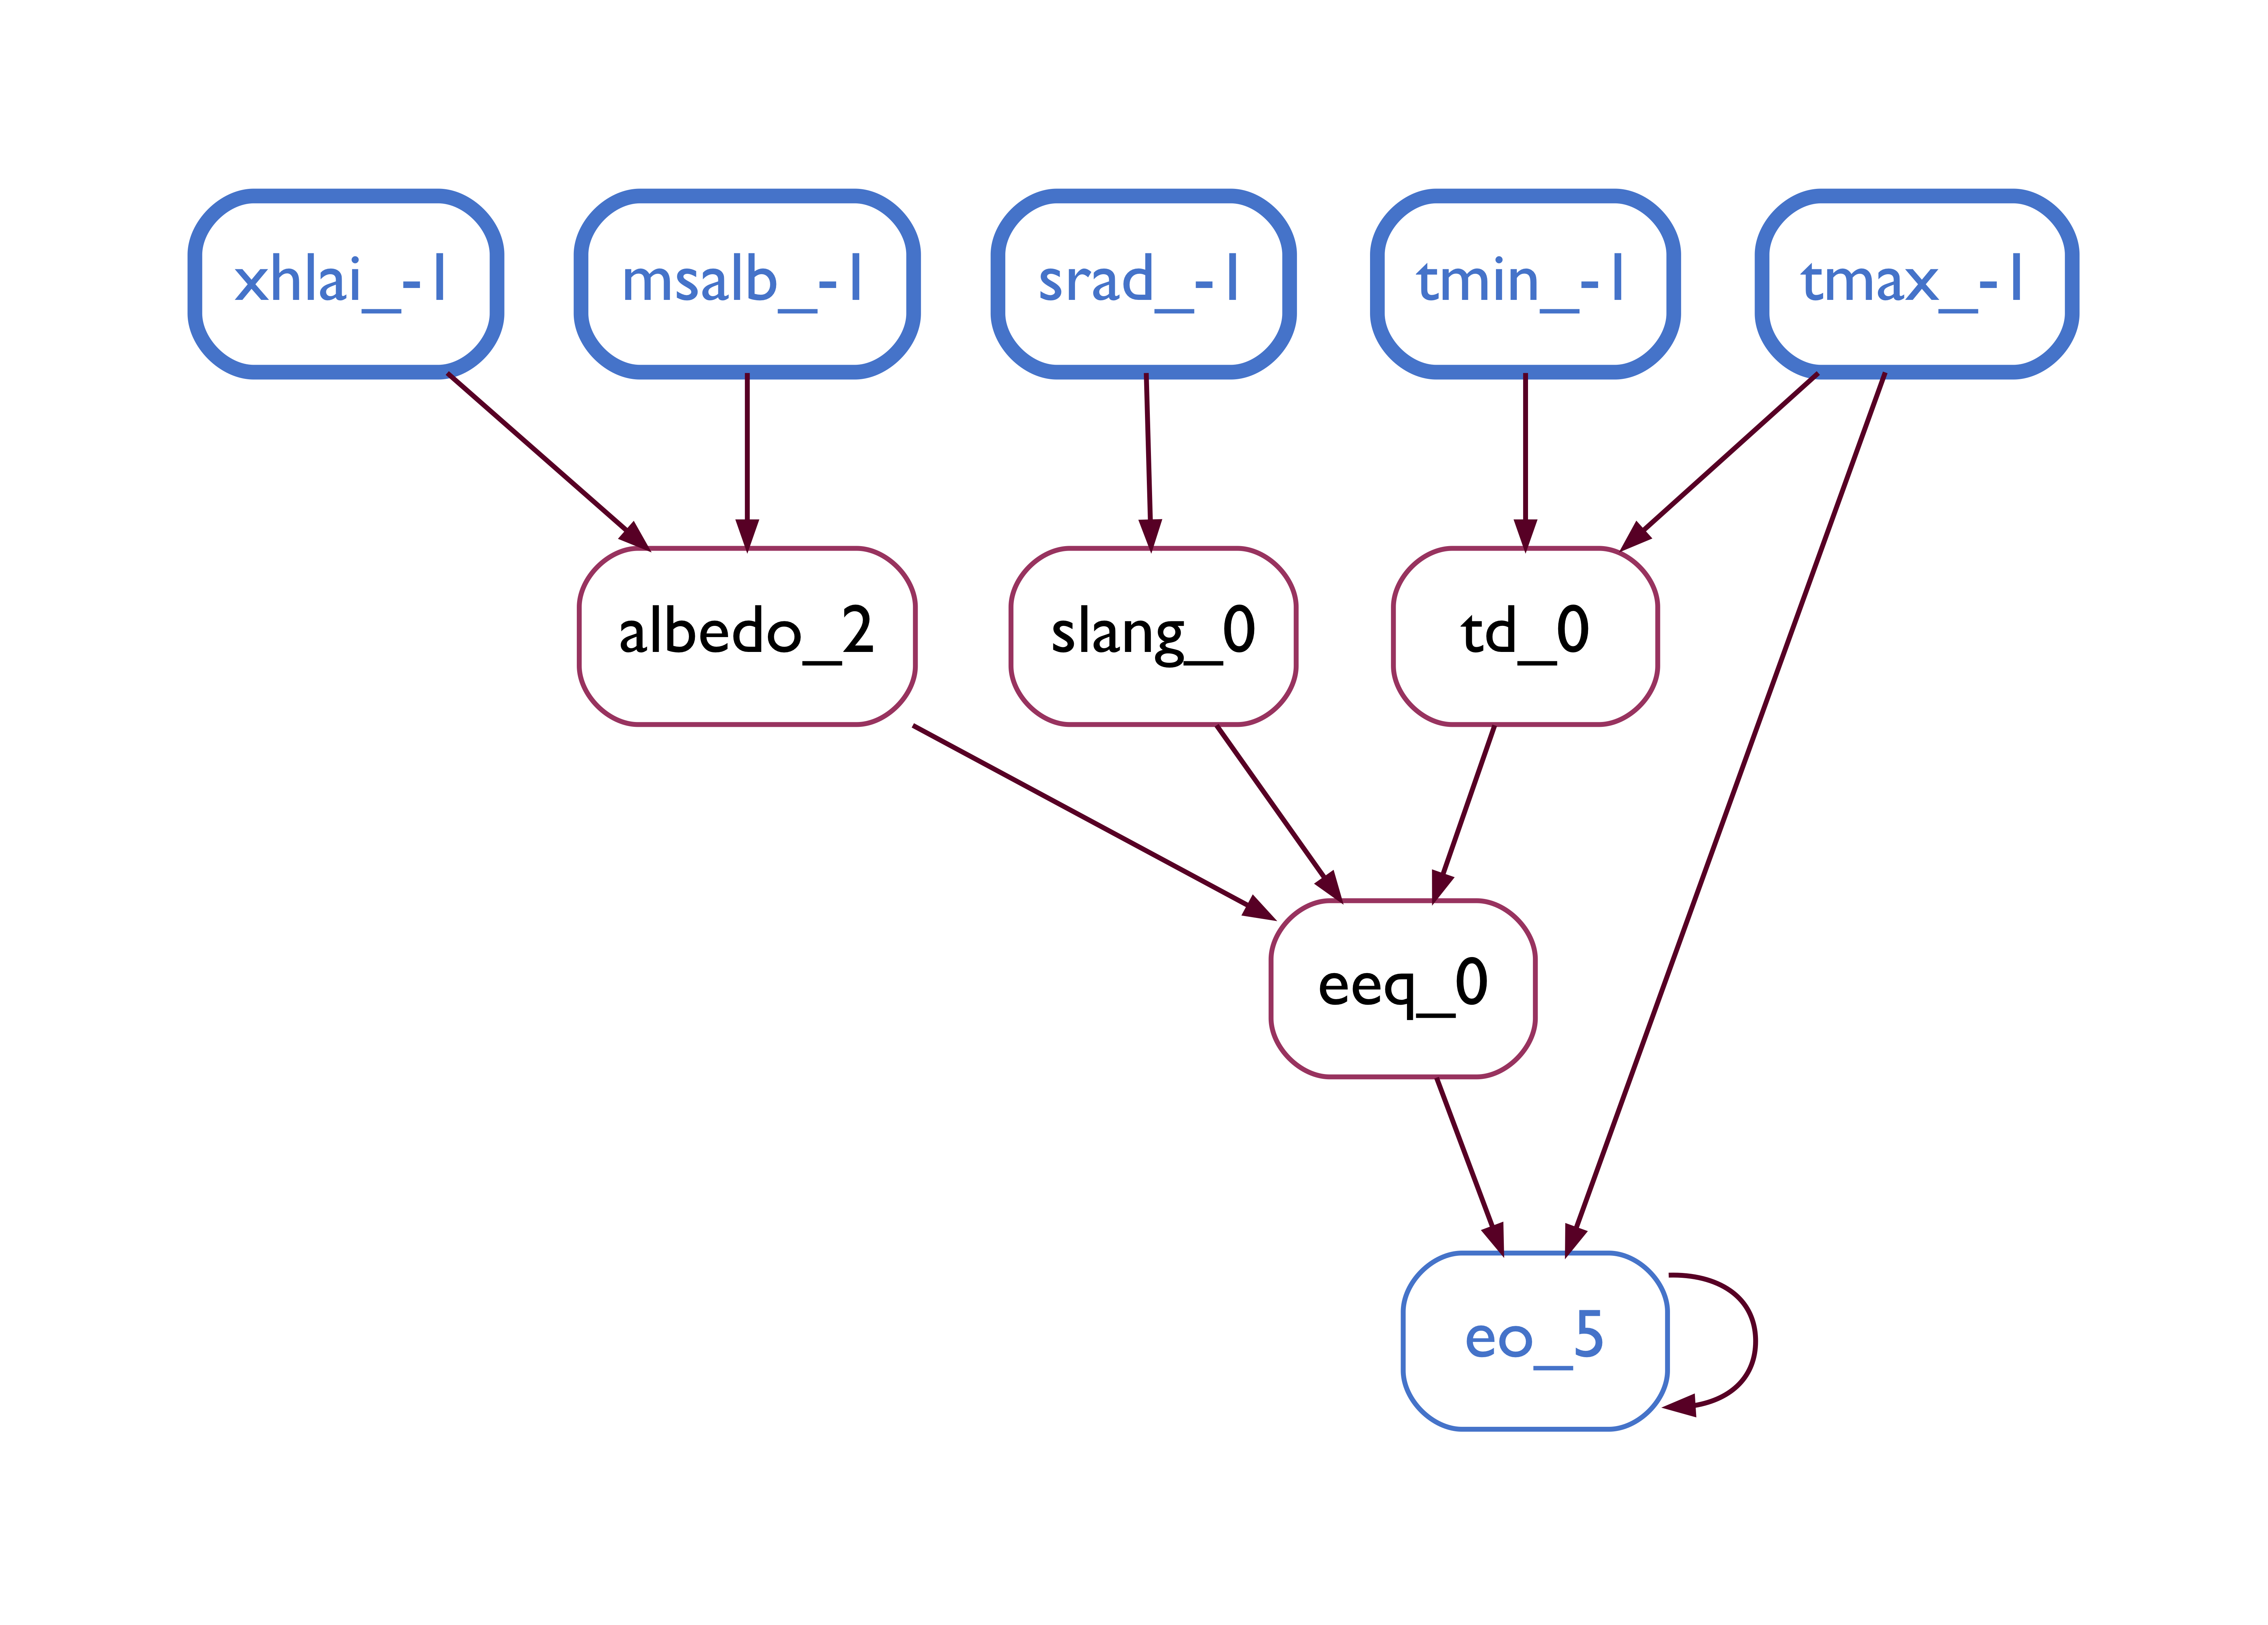
\includegraphics[width=0.75\textwidth]{PETPT_FIB_CAG}\label{fig:petpt_fib}}

  \subfloat[PETASCE FIB CAG]{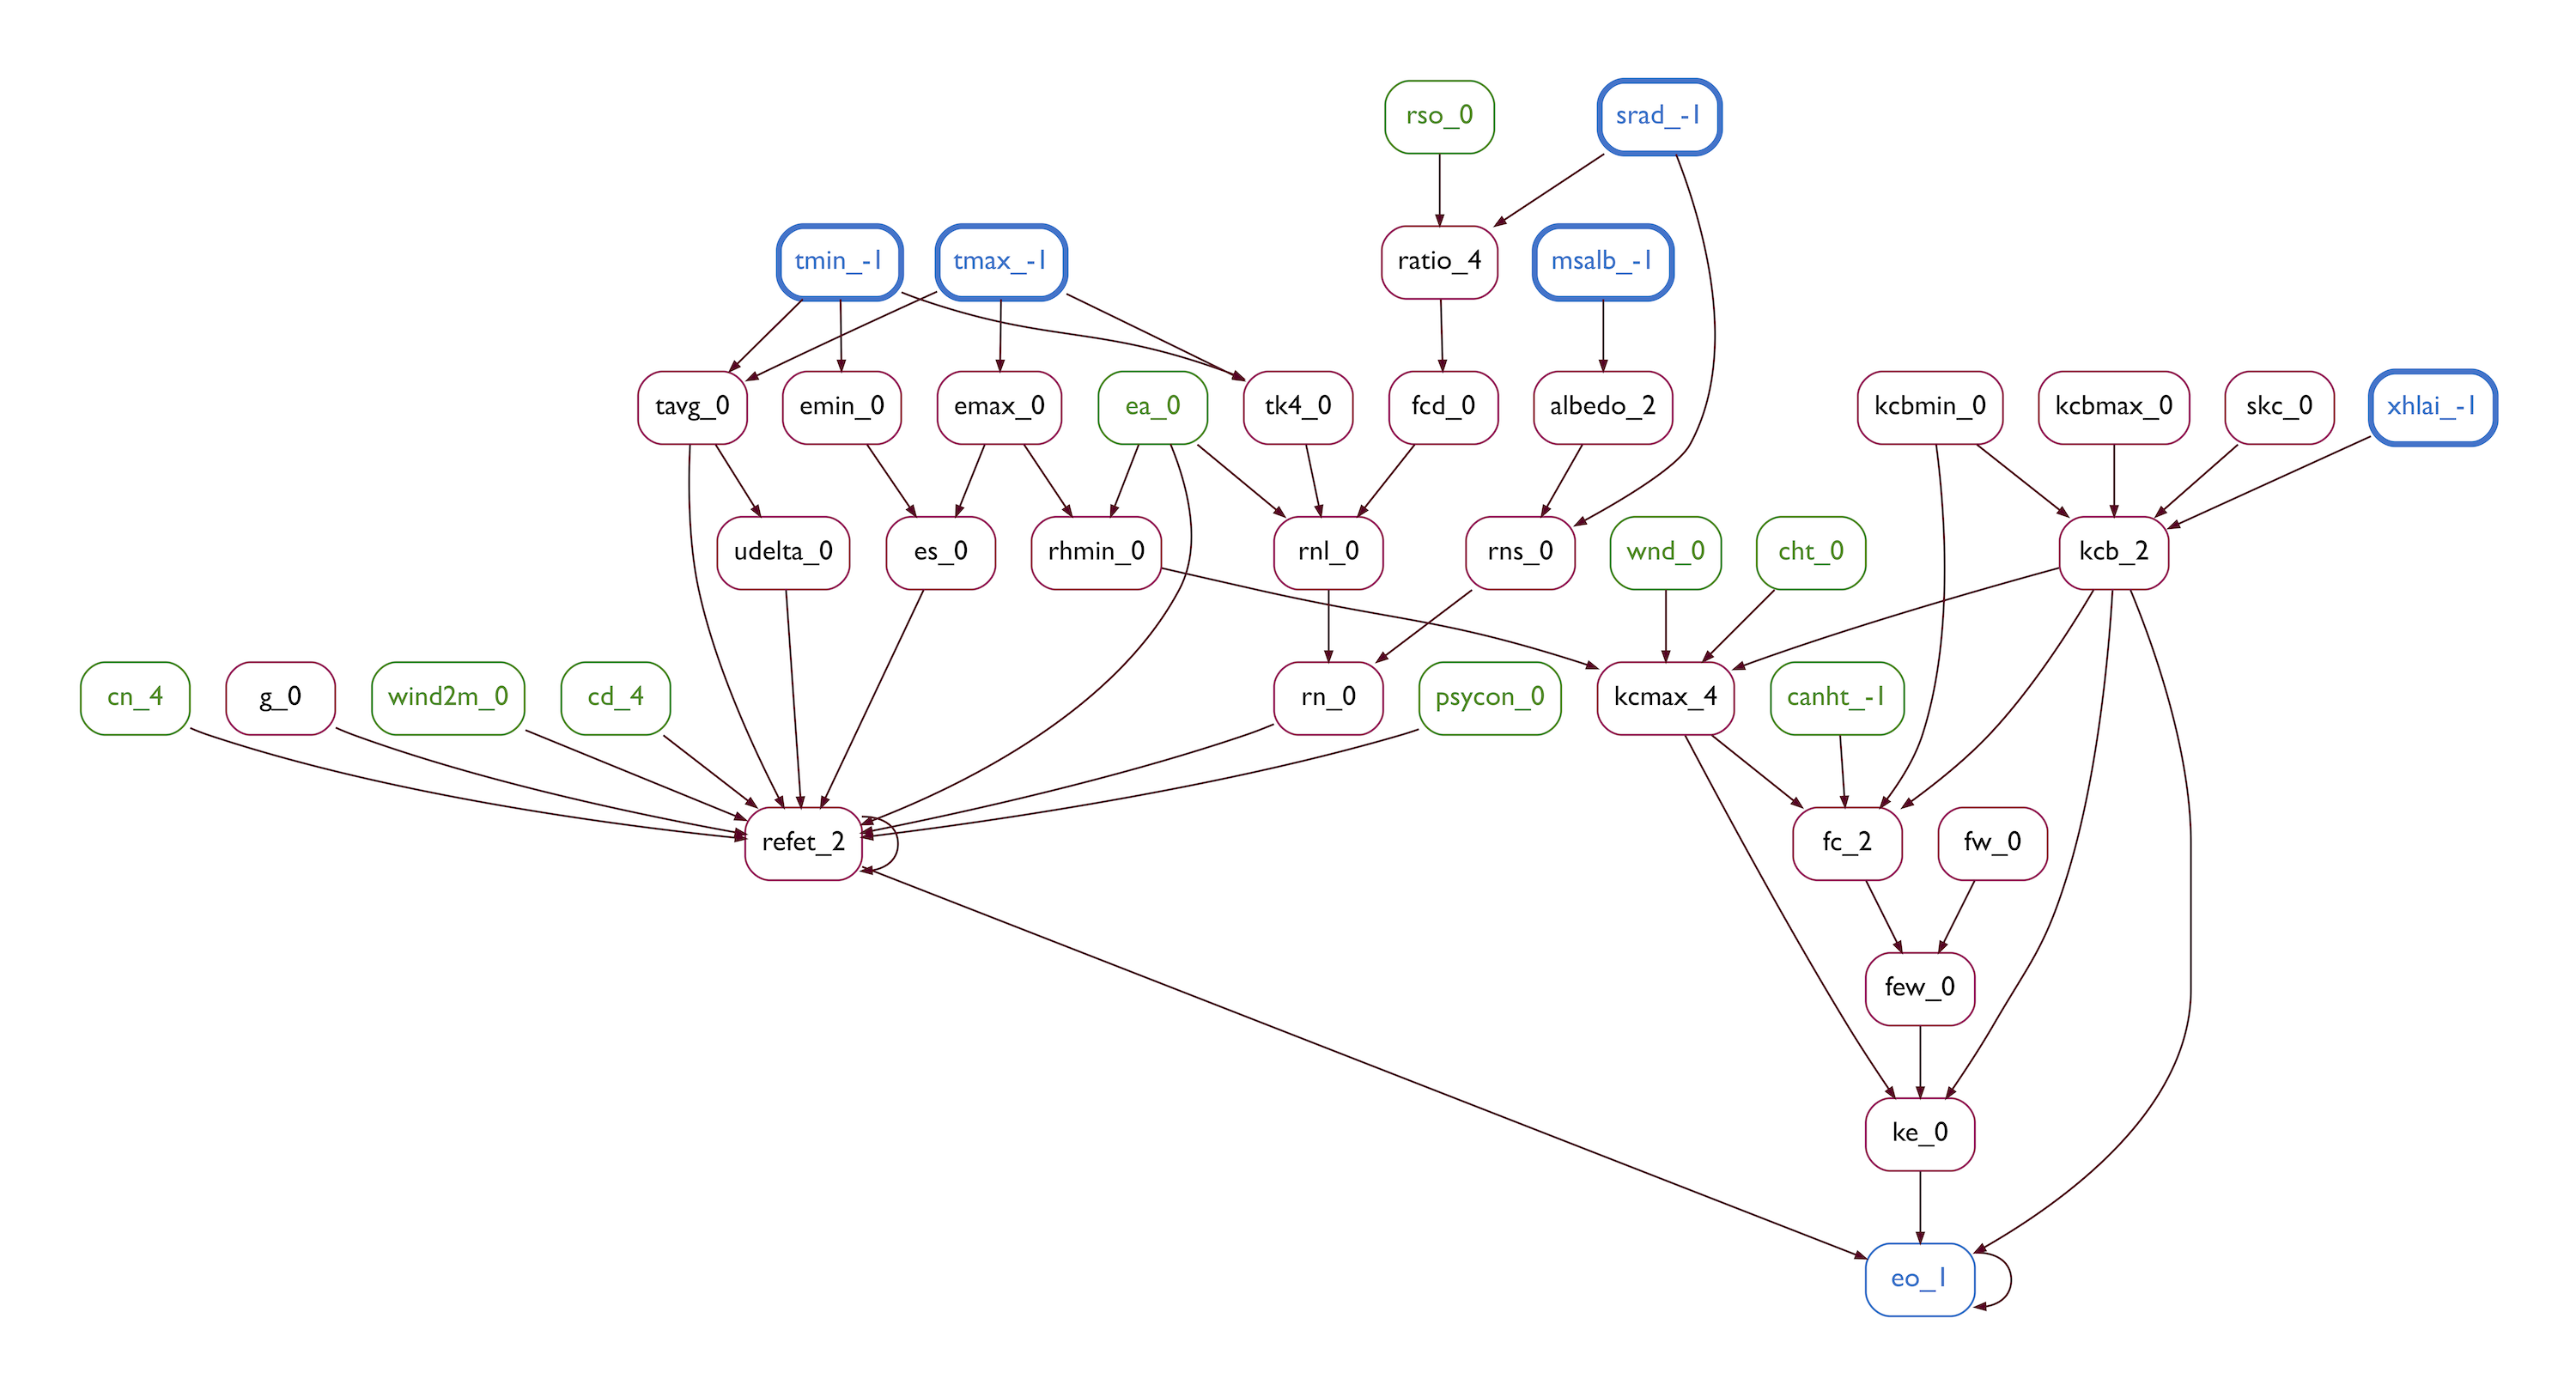
\includegraphics[width=0.75\textwidth]{PETASCE_FIB_CAG_smaller}\label{fig:petasce_fib}}
  \caption[Forward Influence Blanket CAG Examples]{Forward Influence Blanket (FIB) CAGs for the PETPT and PETASCE evapo-transpiration models that depicts the overlap with each other. Note that shared variables are shaded in blue and shared input variables are both shaded blue and bolded. Note that while the PETPT model did not have any variable nodes in the cover set the PETASCE model has several variables in the cover set. These variables are shaded green.}
\end{figure}
\FloatBarrier

% \FloatBarrier
% \begin{figure}[!htbp]
%     \label{petpt_fib}
%     \centering
%     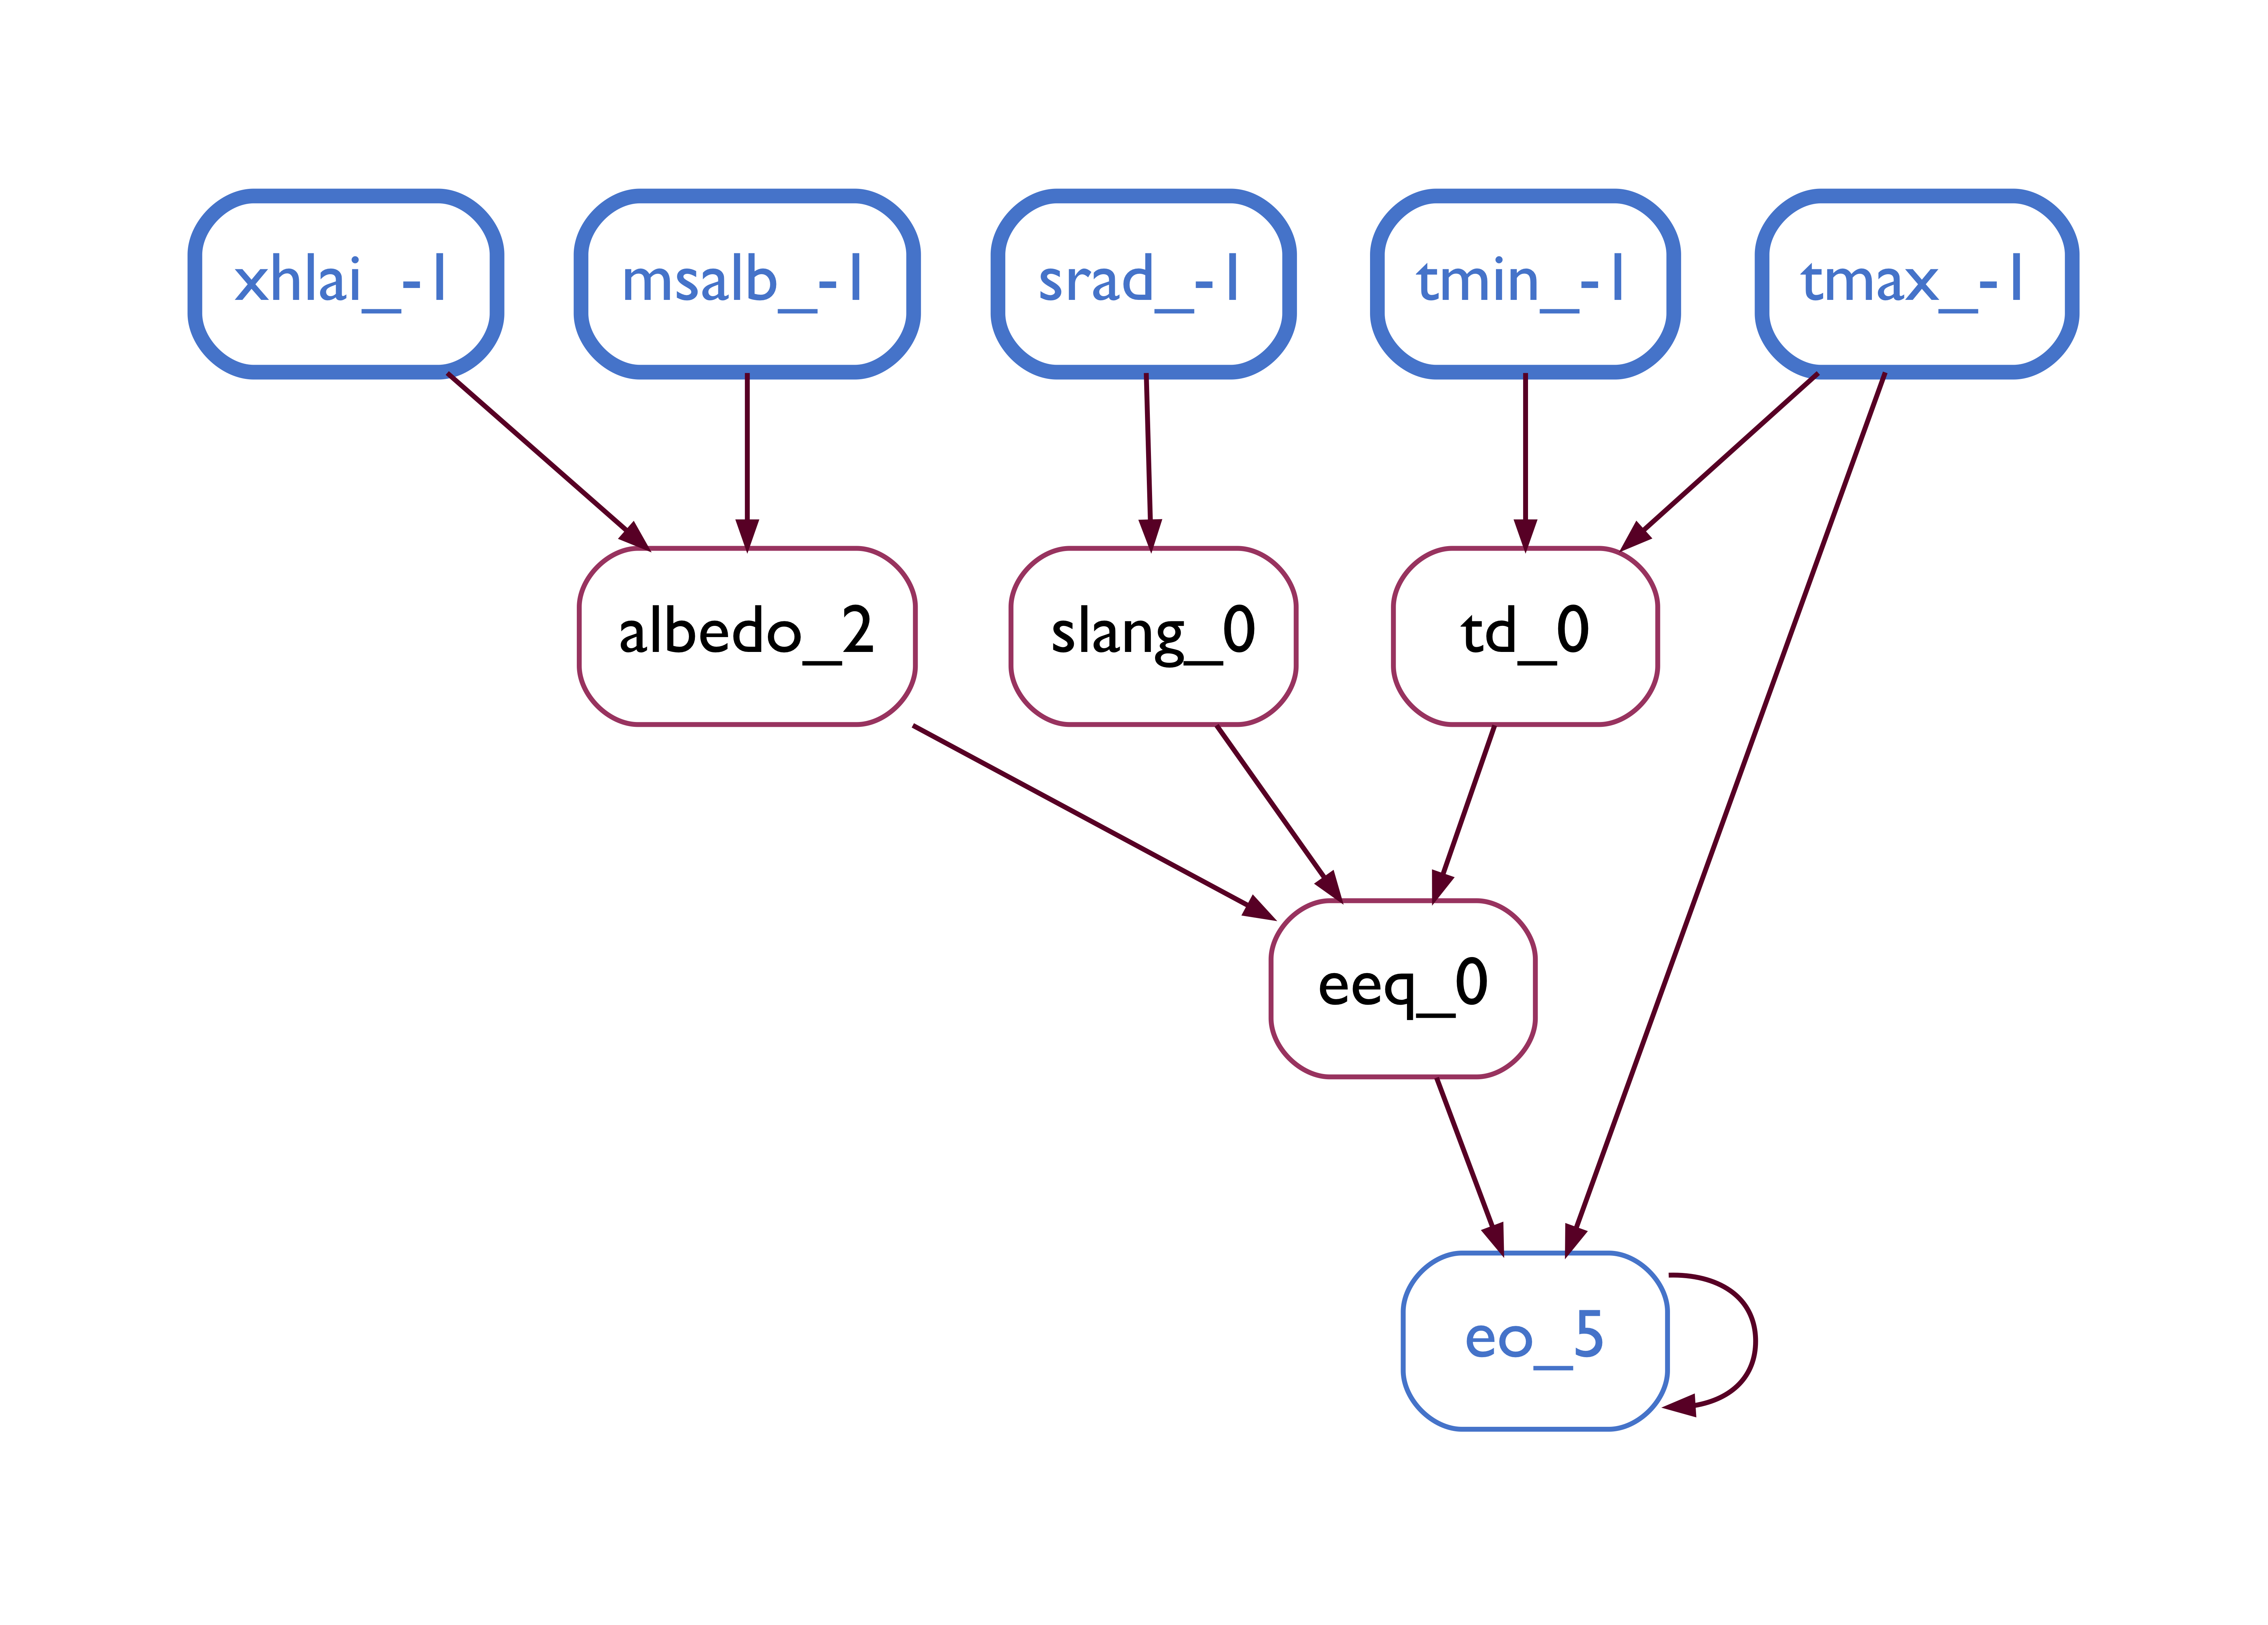
\includegraphics[clip,width=.8\columnwidth]{PETPT_FIB_CAG}%
%     \caption[PETPT FIB CAG]{A Forward Influence Blanket (FIB) for the PETPT model that depicts the overlap with the PETASCE model. Note that shared variables are shaded in blue and shared input variables are both shaded blue and bolded.}
% \end{figure}
%
% \begin{figure}[!htbp]
%     \label{petasce_fib}
%     \centering
%     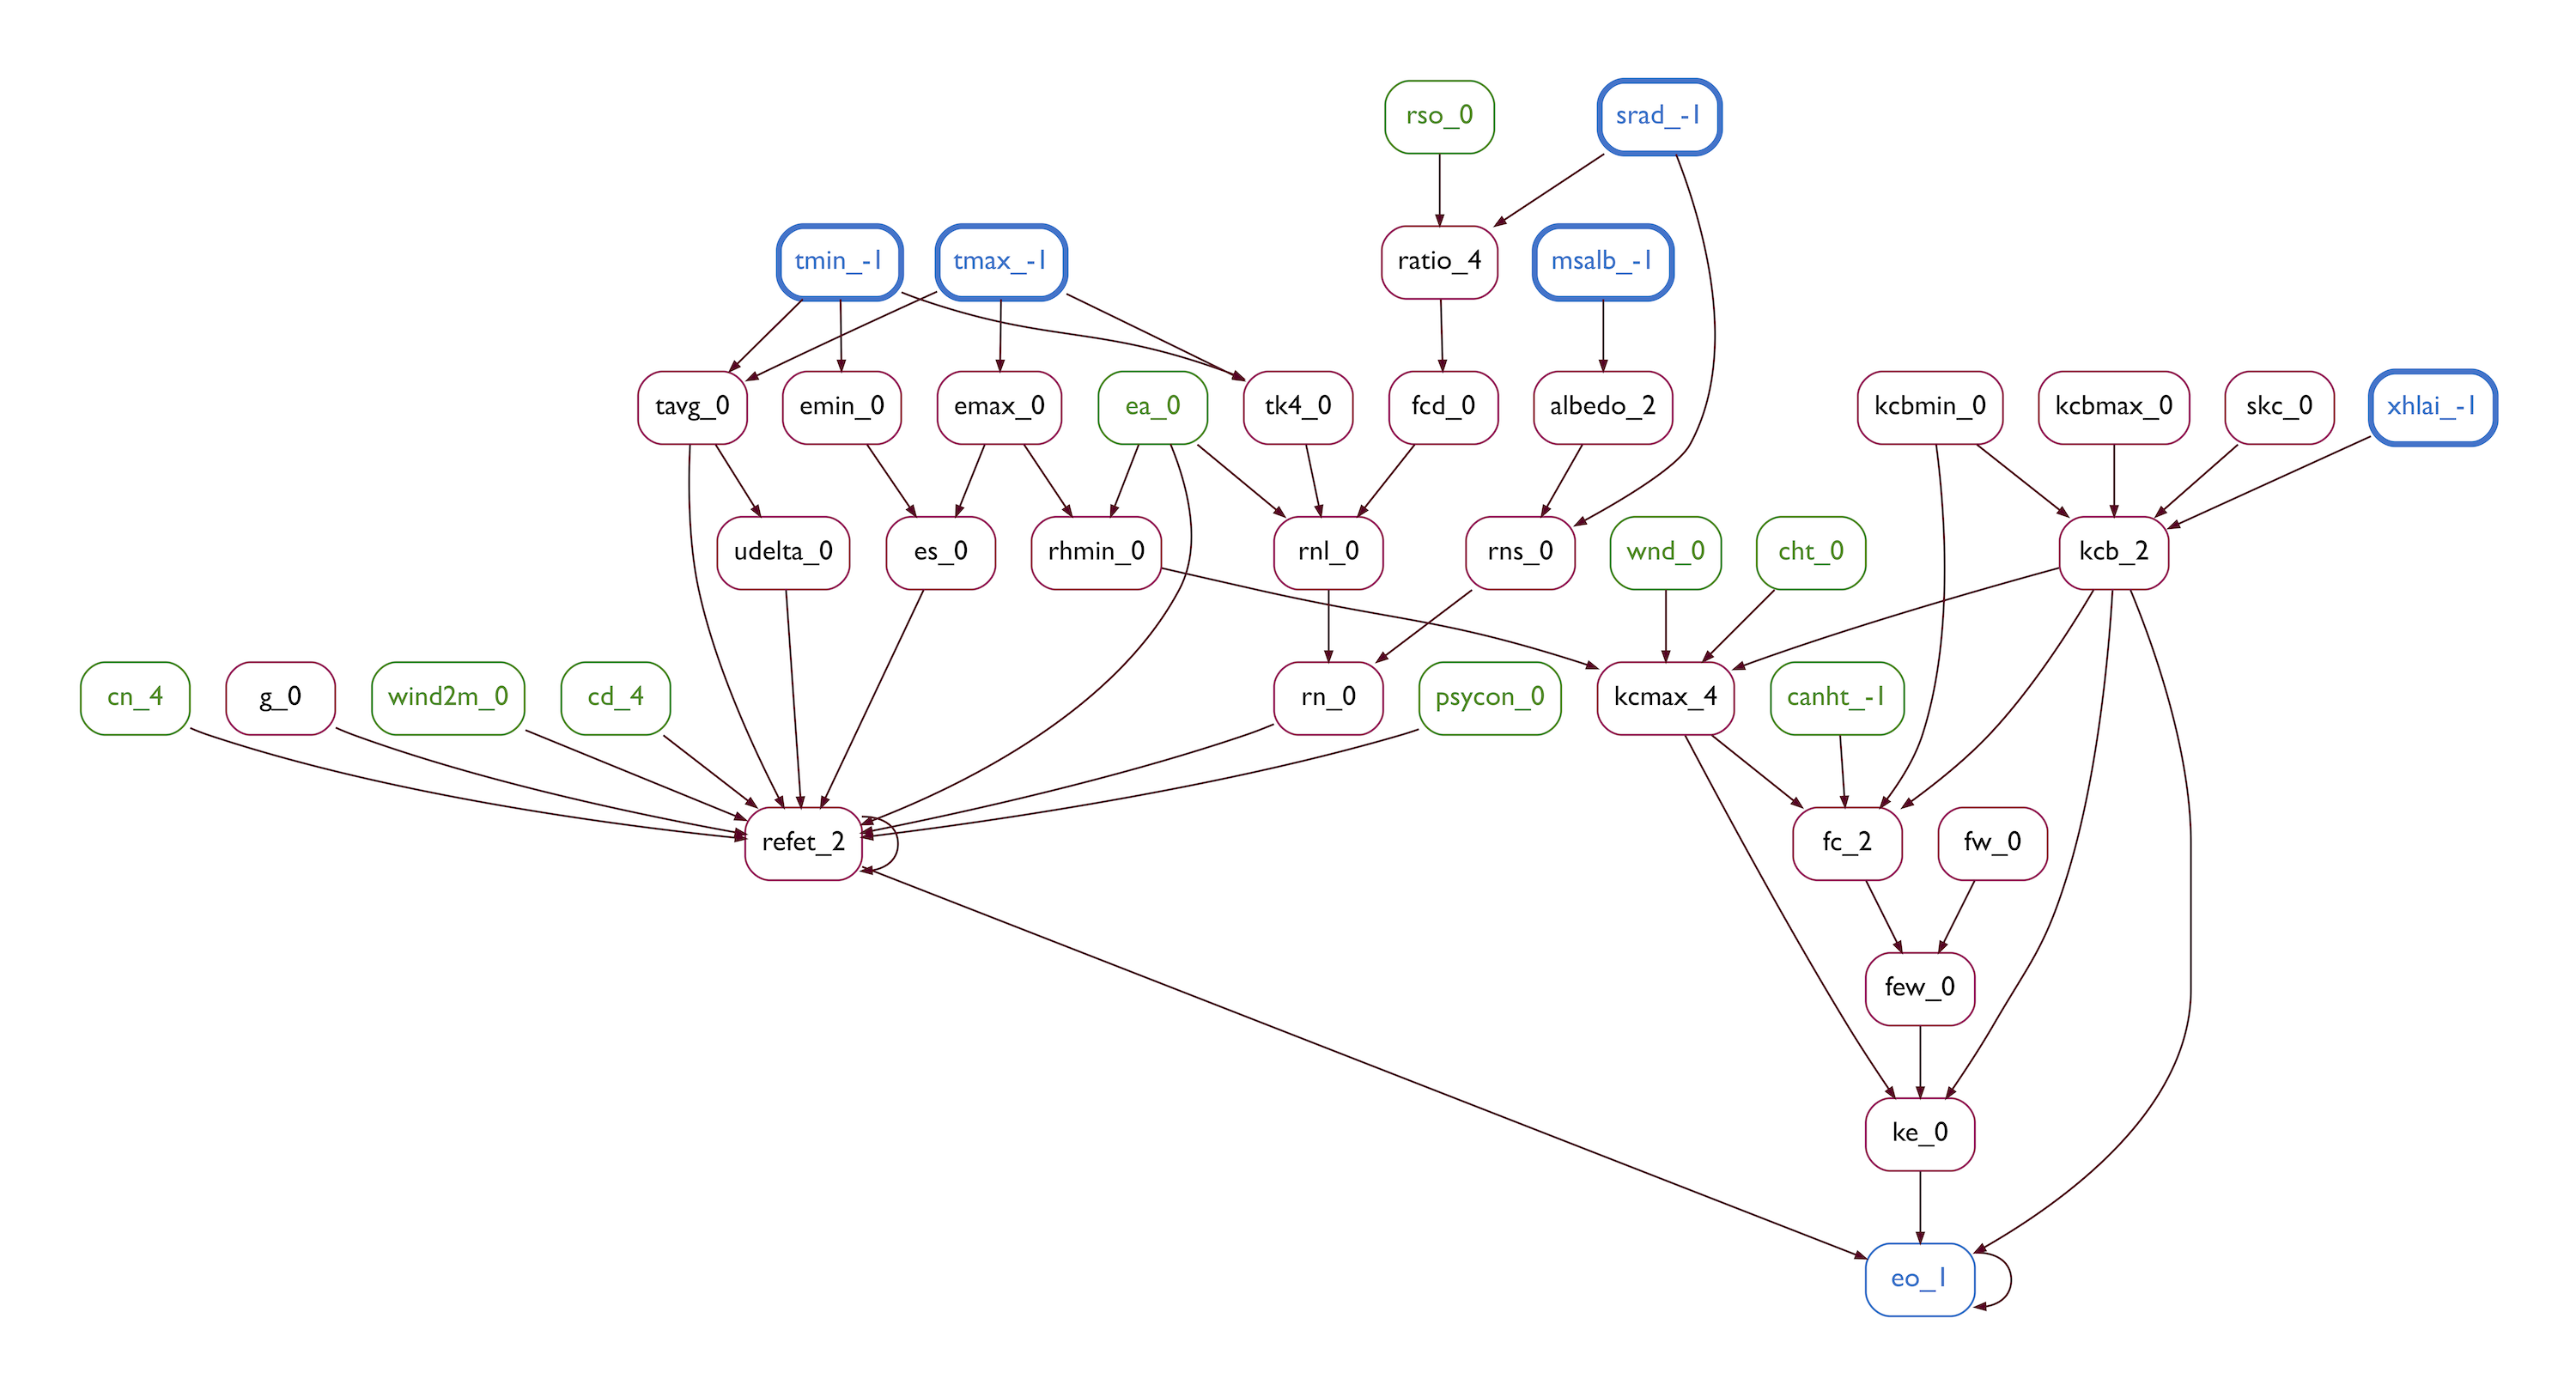
\includegraphics[clip,width=0.8\columnwidth]{PETASCE_FIB_CAG_smaller}%
%     \caption[PETASCE FIB CAG]{A Forward Influence Blanket (FIB) for the PETASCE model that depicts the overlap with the PETPT model. Note that while the PETPT model did not have any variable nodes in the cover set the PETASCE model has several variables in the cover set. These variables are shaded green.}
% \end{figure}
% \FloatBarrier

\subsection{Input Set Execution on a FIB\label{sec:fib_exec}}
In order to execute a FIB the user must provide values for the input variable nodes and values for the cover variable nodes. At execution time, both sets of variable nodes will be populated before beginning to compute the function nodes in the partial order of functions provided by the GrFN computation graph. This is the only difference between computing on a FIB computation graph and computing on a GrFN computation graph.

Execution of a FIB computation graph can be done either with singular preset values for all of the cover variables, or with ranges for each cover variable.
FIB CGs support Torch-aided vectorized computation similar to the GrFN CG structure, and no additional memory constraints are imposed on execution by the FIB class.

\chapter{SELECTED MODEL ANALYSIS STUDIES\label{chapter:analysis_studies}}
The greatest benefit researchers receive from modeling is being able to reason about the uncertainty involved in observing a phenomena of choice.
From the modeling perspective, explicit statements about the uncertainty of a phenomena can be made by adding inputs to the model of the phenomena that represent a source of variance upon the phenomena.
In this section, I will introduce sensitivity analysis methods that I adapt to use in the SMS pipeline as a method for identifying how uncertainty in input variables impacts our uncertainty in output variables within the uniform SMS representation.
Once introduced I will show how the outputs from sensitivity analysis can be used to inform other methods of model analysis, both automatic methods and ones that can be used interactively by the domain modeler.

\section{Structural Model Analysis\label{sec:structural_analysis}}

\subsection{Overlap Identification\label{sec:overlap_identification}}
While analytical methods can provide a large amount of useful information to modelers about a single model, the real benefit of the AutoMATES system comes from the ability to automate comparisons among competing models. Competing models can be identified from the output variables of their computation graphs. After identifying a selection of competing models the comparison phase can begin.

For any two competing models of the same phenomena the comparison phase consists of the following:

\begin{enumerate}
  \item Identify the overlap between the variables in each models computation graphs. This corresponds to overlap in observable observable phenomena.
  \item Extract the sub computation graphs for each model based on the variable node overlap.
  \item Perform analysis on the overlapping computation graphs and compare the results with the analysis results from the models whole computation graphs.
\end{enumerate}

In order to accomplish the tasks outlined above, I will introduce a new construct, known as a Forward Influence Blanket (FIB). A FIB is a specific instance of a Markov blanket \citep{pearl2009causality}, derived from a GrFN computation graph, that can be used for forward analysis.  % TODO: possibly define forward analysis and markov blanket
After the completion of these tasks the information gained from the comparative study of these models can be added to the final model report, or used for automatic model selection. In this chapter I discuss model comparison in terms of two models compared directly with one another. At the end of the chapter I will elucidate on the necessary steps to generalize this form of binary model comparison to a set of $N$ models.

\subsubsection{Identifying a Forward Influence Blanket\label{sec:fib_creation}}
Imagine the structure of two computational models of the same phenomena in the most general sense. We can say with certainty that both models will have the same output variable, namely the variable that represents the phenomena of interest. From this there are three options for how the set of input variables between the two computational graphs can overlap. The least interesting option is that the two models could share no inputs variables. This would mean that the computations involved in each model are wholly independent and could be combined if necessary in a trivial manner, at least at the input level. The more interesting option is that a subset of the inputs are shared between the two models. This entails that the models will make use of the same data, though the computations used to transform that data into a model output will almost certainly differ. It is possible that the set of input variables will overlap exactly between the two models; however, it is much more likely that there will be some input variables that are not contained in both. In the following subsections I will discuss how to build a computation graph that represents the computation present in a GrFN that corresponds to utilization of shared variable nodes with another model.

% TODO: Add material about Shared Structure Identification here
The shared structure components of a FIB for two models of the same phenomena are identified using the following strategy.
By definition the models share the same output variable node.
Therefore any shared structure will be within the range of a shared variable node, either an input variable or an inner variable node, and all the full computation path to the output node.
A set of shared nodes between the two graphs can be discovered using node name matching on the grounded node names.
This is done upon the CAG view of the GrFN CG so that variable nodes are only matched once and not once per update recorded in the overall CG.
Using the set of shared nodes and the output node we can discover all computation paths that lead to the output node by doing an exhaustive path search from each shared node to the output node \citep{sedgewick2002algorithmsInC}.
Combining the outputs from all of these paths together gives us the shared portions of each GrFN CG that serve as the basis for each models FIB.

% TODO: The section discusses Cover Set Variables
The key aspect of a FIB that distinguishes it from a GrFN computation graph is that the portions of the original computation graph that are not shared between the two models under comparison are pruned.
In order to ensure that the resulting models are still executable, variable nodes representing new inputs to the FIB computation graph must be retained.
This set of variables has been identified as the cover set.
Forming this cover set and adding it to the shared overlap portion of each GrFN CG as mentioned above is the last step necessary to fully create the FIB for each model.
Identifying a variable as being a member of the cover set stems from the initial shared graph structure extracted from the original GrFN CGs.
All nodes along the shared structure must be compared to the node structure in the original CG.
If any nodes are missing a branch that is present in the original CG then the immediate parent of the node must be added to the set of cover nodes and is grafted on to the FIB.
Once the set of cover nodes are added to the shared graph structure the FIBs for each model are complete.
To visualize what a FIB looks like for both a small and large CG we have added the FIBs that denote the overlap between the two evapo-transpiration models.

\FloatBarrier
\begin{figure}[!tbp]
  \centering
  \subfloat[PETPT FIB CAG]{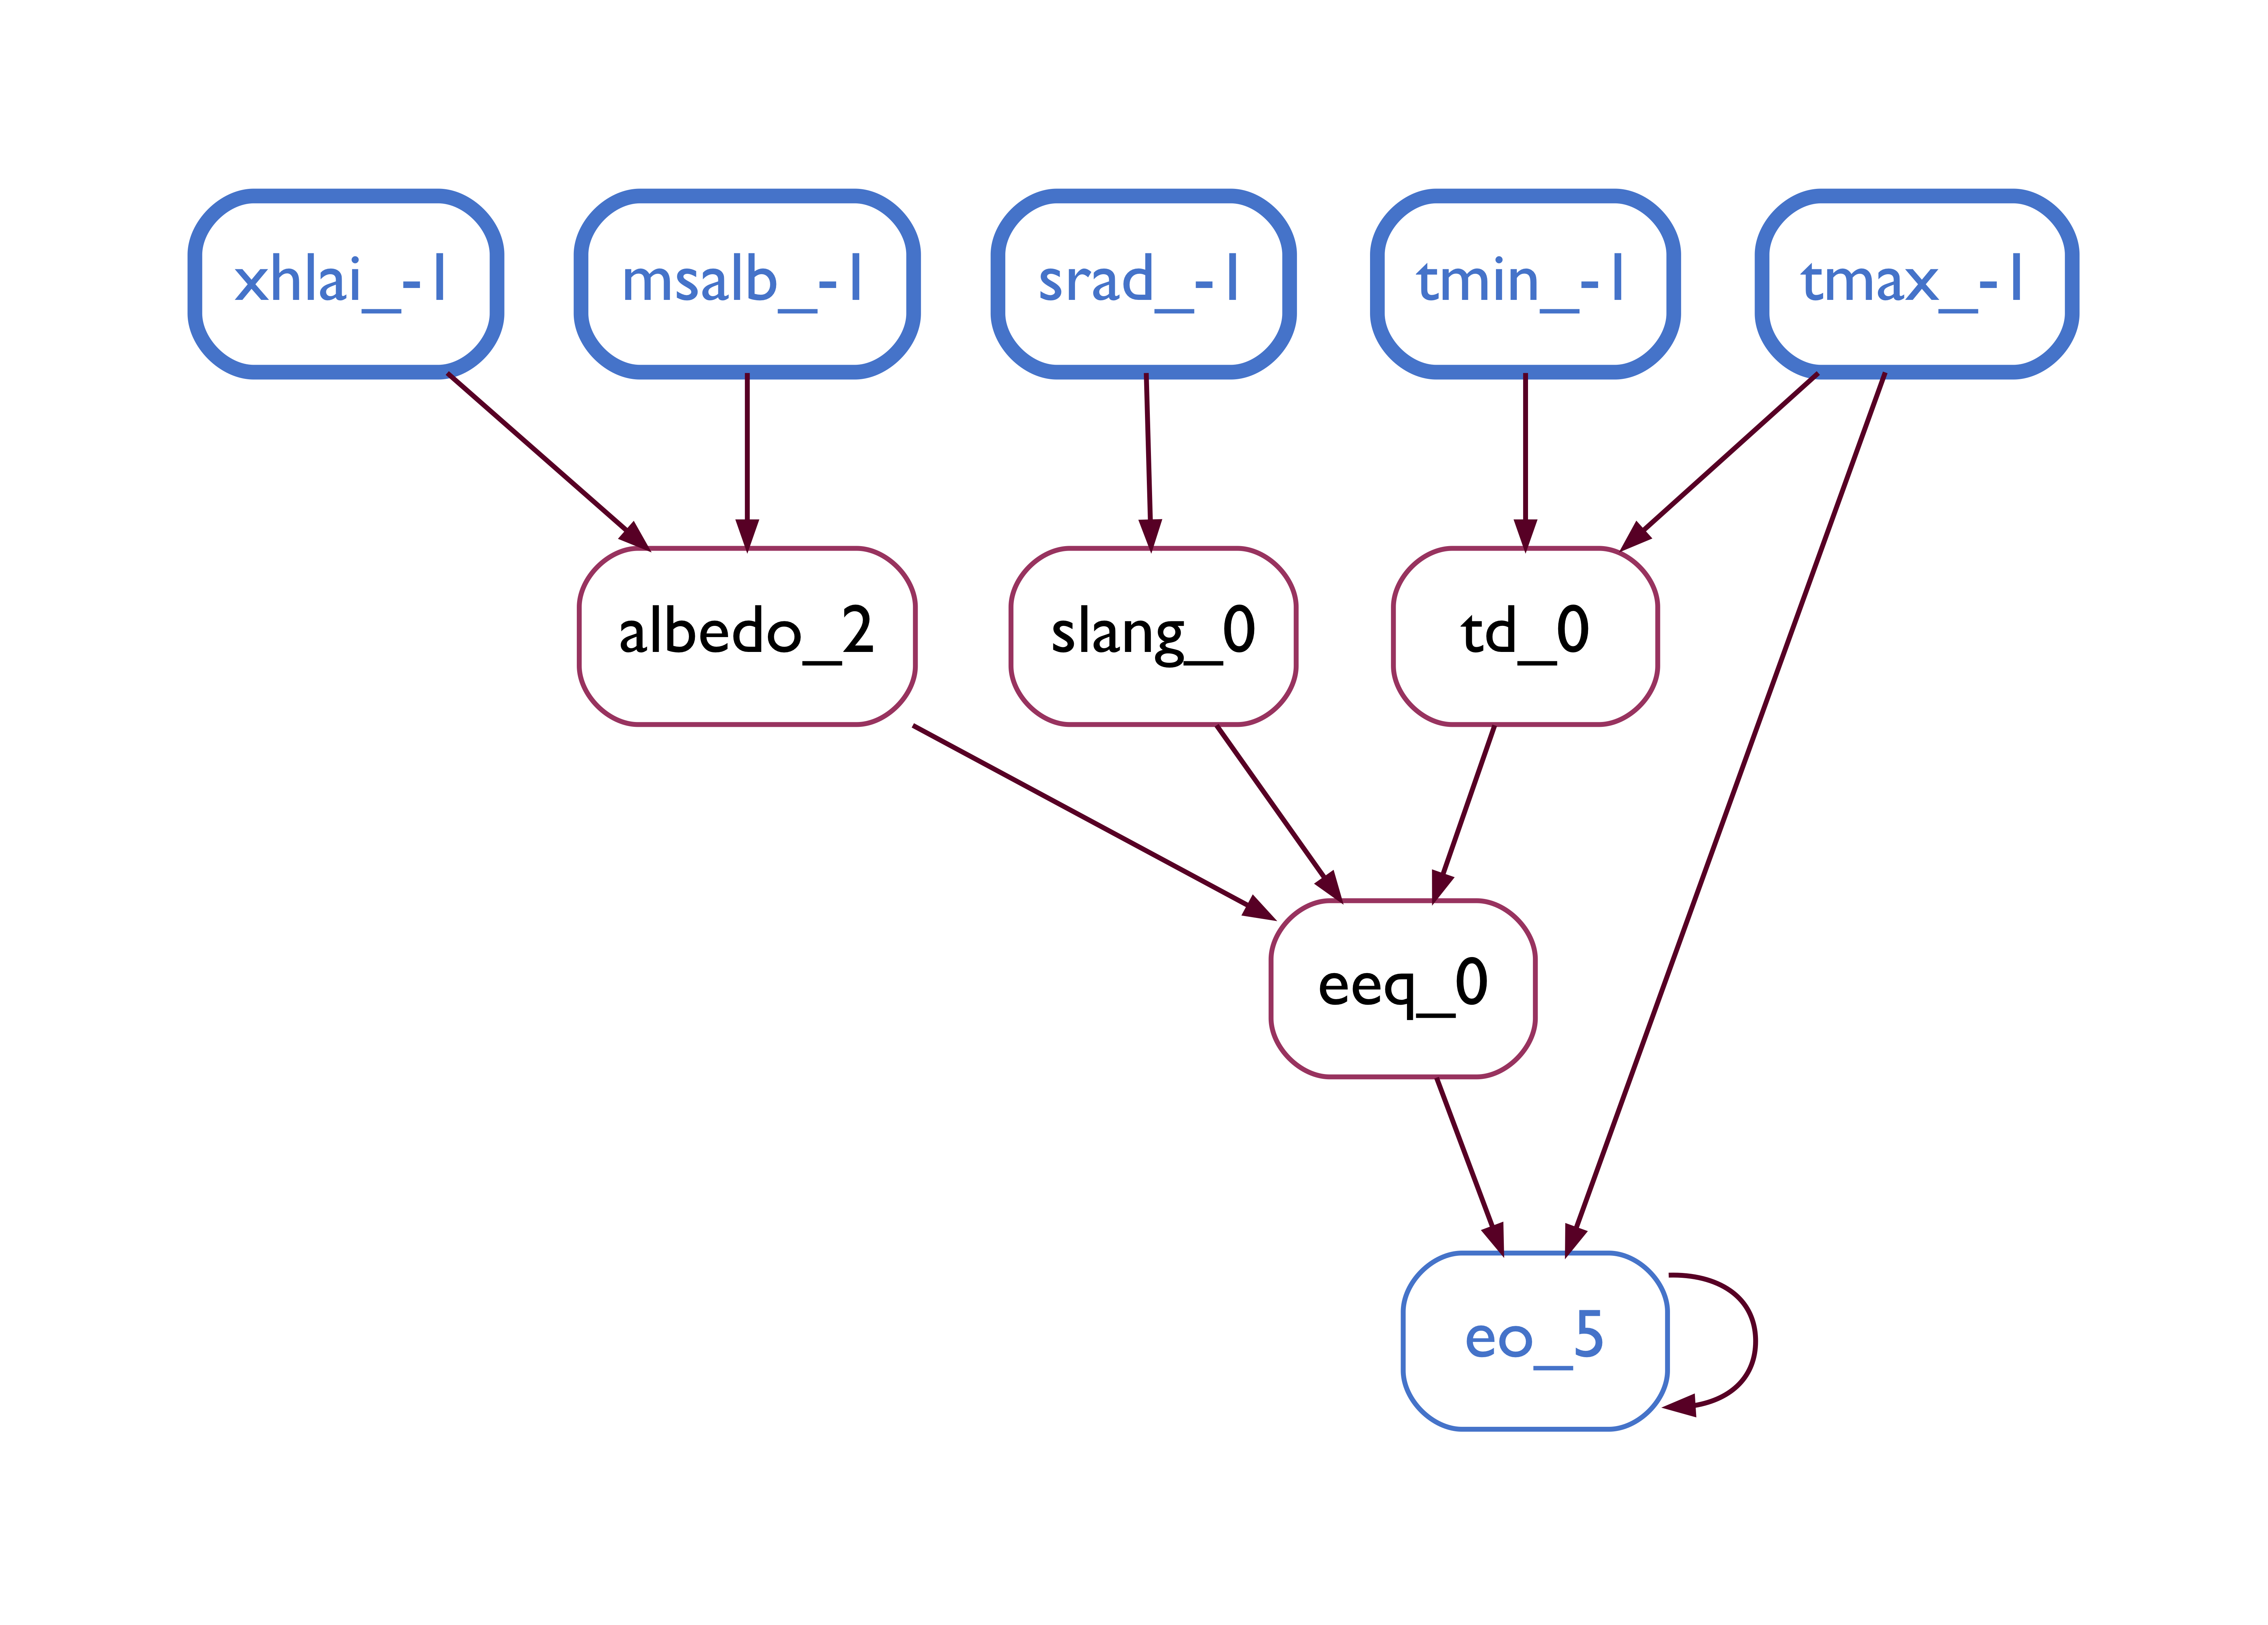
\includegraphics[width=0.75\textwidth]{PETPT_FIB_CAG}\label{fig:petpt_fib}}

  \subfloat[PETASCE FIB CAG]{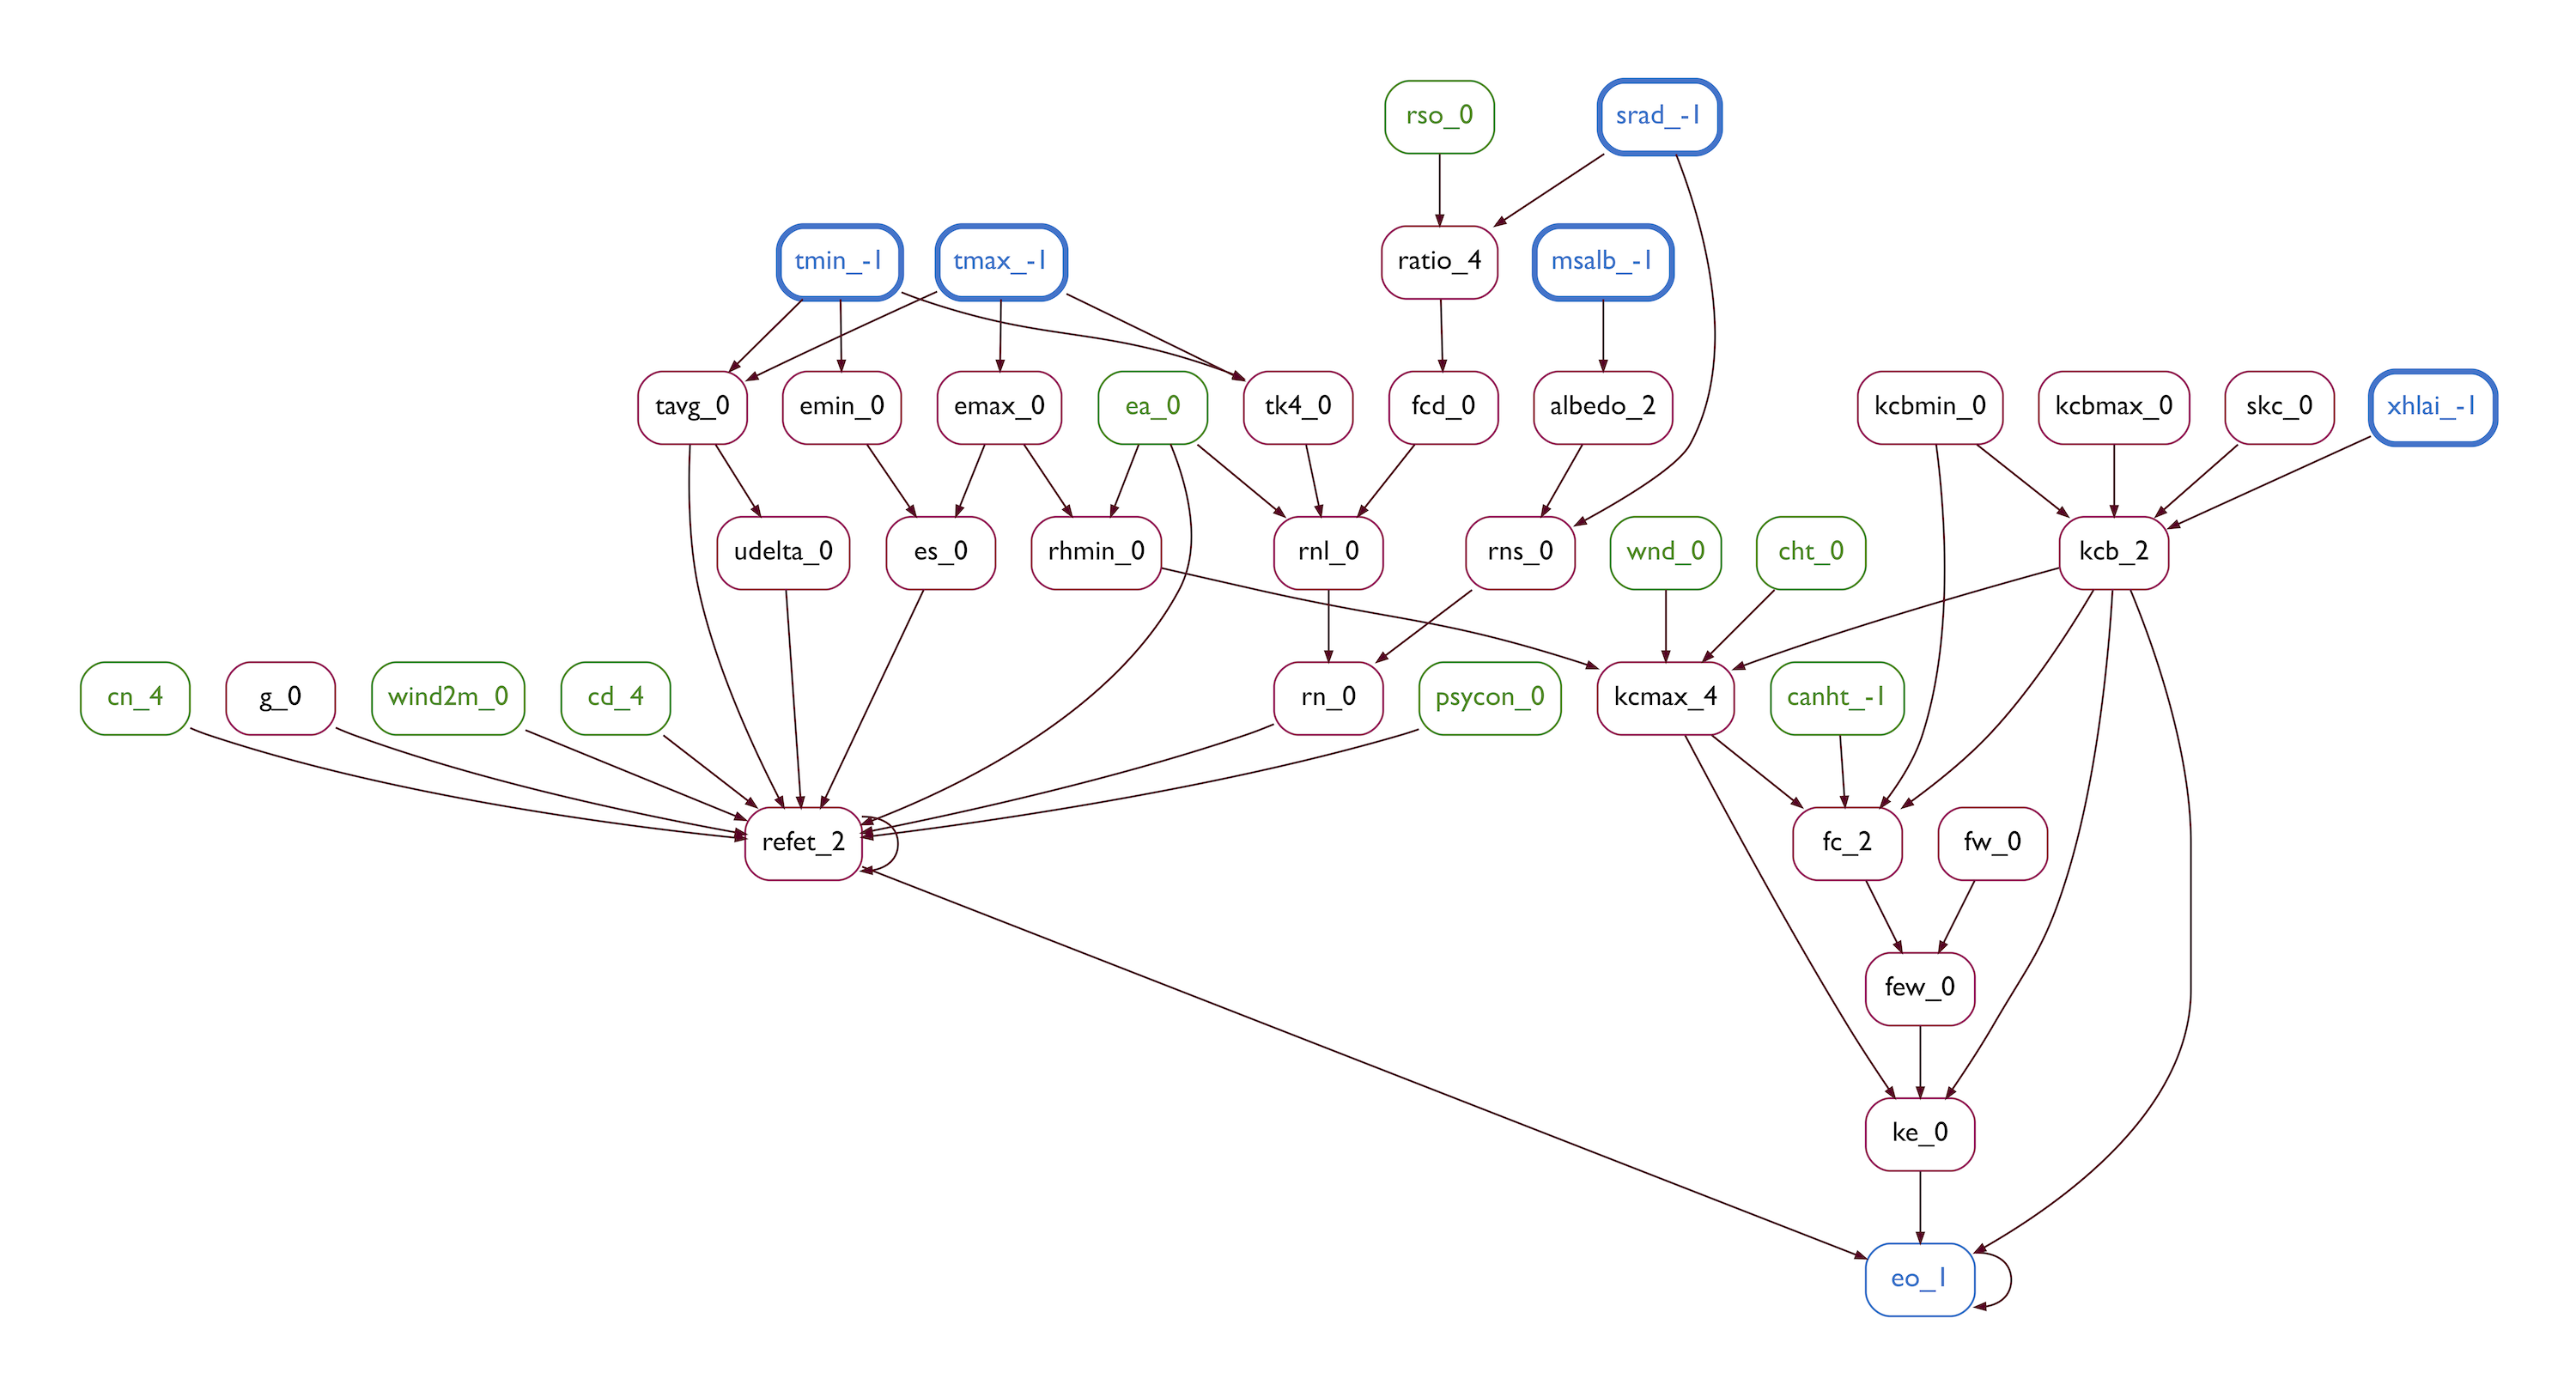
\includegraphics[width=0.75\textwidth]{PETASCE_FIB_CAG_smaller}\label{fig:petasce_fib}}
  \caption[Forward Influence Blanket CAG Examples]{Forward Influence Blanket (FIB) CAGs for the PETPT and PETASCE evapo-transpiration models that depicts the overlap with each other. Note that shared variables are shaded in blue and shared input variables are both shaded blue and bolded. Note that while the PETPT model did not have any variable nodes in the cover set the PETASCE model has several variables in the cover set. These variables are shaded green.}
\end{figure}
\FloatBarrier

\subsubsection{Input Set Execution on a FIB\label{sec:fib_exec}}
In order to execute a FIB the user must provide values for the input variable nodes and values for the cover variable nodes. At execution time, both sets of variable nodes will be populated before beginning to compute the function nodes in the partial order of functions provided by the GrFN computation graph. This is the only difference between computing on a FIB computation graph and computing on a GrFN computation graph.

Execution of a FIB computation graph can be done either with singular preset values for all of the cover variables, or with ranges for each cover variable.
FIB CGs support Torch-aided vectorized computation similar to the GrFN CG structure, and no additional memory constraints are imposed on execution by the FIB class.

\section{Functional Model Analysis\label{sec:functional_analysis}}

\subsection{Global Sensitivity Analysis\label{sec:sens_analysis}}
A powerful tool used by modelers to quantify the uncertainty present in models is global sensitivity analysis. Broadly speaking, global sensitivity analysis is the study of how variance in the inputs of a model affect the variance, or uncertainty in the output of the model. Since the goal of the SMS pipeline is to provide modelers with a tool select a model that lowers the amount of uncertainty in estimation of a given phenomena we have chosen to use sensitivity analysis in order to evaluate the extracted models.

For this thesis we employ variance-based methods of sensitivity analysis.
% TODO: give a good definition of variational methods of sensitivity analysis
Variance-based methods of sensitivity analysis focus on the computation of sensitivity indices. Sensitivity indices are numerical values assigned to each model input, or set of inputs, that denote how sensitive the output of the model is to that input, or set of inputs. The first order sensitivity index, commonly denoted by $S_1$, notates the sensitivity of the model output from each individual input. Similarly the second order sensitivity index, commonly denoted $S_2$, notates the sensitivity of the model output from each pair of model inputs. This pattern continues for any given model for all higher order sensitivity indices.
The final sensitivity index is the total sensitivity index, commonly denoted as $S_T$. This index has an entry that corresponds to each model input. Each entry tracks the total amount of sensitivity on the model output contributed by the input as a portion of the first, second, and all higher order sensitivity indices.

While other methods of sensitivity analysis exist, such as Variogram Analysis of Response Surfaces (VARS), the variance-based methods fit well within the scope of our problem domain as we are conducting sensitivity analysis over probabilisitic models.
While the VARS method does claim a significant faster computation time, it does not reveal as much information about the affects of model inputs upon the model output.
This is due to the lack of pairwise-information that the variance-based methods are able to capture.
In the following subsections I will discuss Sobol analysis, developed by \citet{sobol2001globalSA}, that will be used to perform variance-based sensitivity analysis upon the extract scientific models and I will address how it has been adapted for use by the SMS pipeline.

\subsubsection{Sampling Inputs with the Sobol Sequence\label{sec:sobol_seq}}
Sobol analysis is the most widely used version of variance-based sensitivity analysis. The Sobol analysis method gets its name from the sampling method used during analysis. Samples for Sobol analysis are drawn from the Sobol sequence. Defining the precise nature of the Sobol sequence is beyond the scope of this masters thesis; however, we can observe how the Sobol sequence aids sensitivity analysis by observing the differences between draws from the Sobol sequence and draws from a random sample. A visualization of the difference is shown below in figure \ref{fig:sobol_seq_vis}.

\FloatBarrier
\begin{figure}[!htbp]
    \label{fig:sobol_seq_vis}
    \centering
    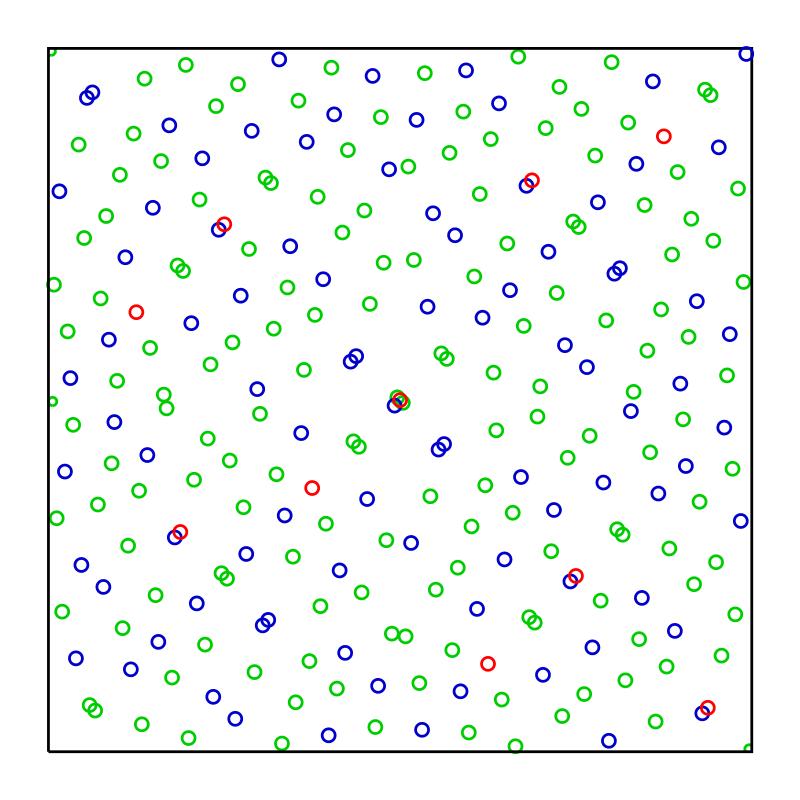
\includegraphics[width=.45\textwidth]{sobol_samples}\hfill
    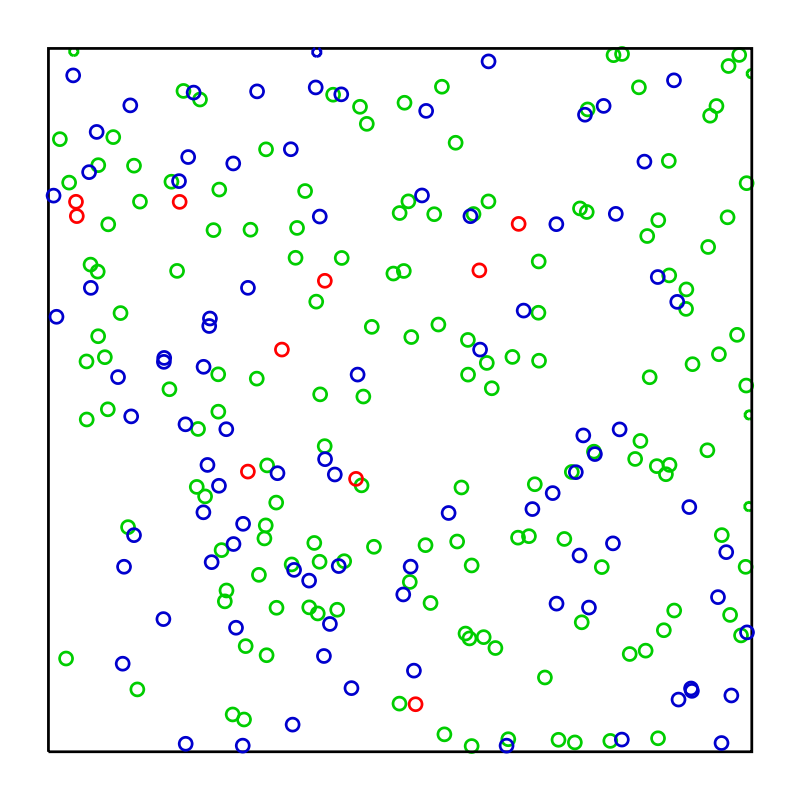
\includegraphics[width=.45\textwidth]{random_samples}
    \caption[Sobol Sequence Visualization]{A visualization of 1000 draws from the Sobol Sequence (left) paired with 1000 randomly drawn points (right) in two dimensions. For both images the first 10 draws are colored red, the remaining first 100 draws are colored blue, and the remaining 1000 draws are colored green. Images created by James Heald, distributed under a CC BY-SA 3.0 license.}
\end{figure}
\FloatBarrier

Notice that the red, blue, and green draws from the Sobol sequence are much more evenly dispersed across the sample space than the same draws from a uniform random sample. This allows the Sobol sampling method to achieve much better coverage of the search space, while still maintaining some variability in sample locations. The SMS pipeline employs a variant of the Sobol sequence, introduced by \citet{saltelli2002ImprovedSobolSeq}, which is designed to minimize the error when utilizing the samples to calculate the sensitivity indices of a function.

\subsubsection{Sensitivity Index Computation\label{sec:si_comp}}
% TODO: Add more material here to introduce the section
The sample matrices that must be computed for analysis are defined in algorithm \ref{fig:sobol_sample_alg}. We can see that this sampling algorithm draws $N$ samples of $d$ dimension from the Sobol sequence and then creates $N(d+2)$ samples total to be evaluated by the model. The matrices returned from the sampling step can then be evaluated using the model computation graph. These evaluations will be represented as $f(A) \text{, } f(B) \text{, } f(\textbf{A}_{B}) \text{, and } f(\textbf{B}_{A})$. Once the evaluation step is completed, the evaluations will be analyzed according to the Sobol analyzer. The Sobol analyzer computes three different sensitivity indices using approximation equations for \citet{saltelli2010varianceSA} improved method of Sobol analysis.

\begin{figure}
  \label{fig:sobol_sample_alg}
    \begin{algorithmic}[1]
      \State $d \gets $ amount of input variables
      \State $N \gets $ amount of desired samples
      \State $R \gets $ set of sample space ranges for all $d$ input variables
      \State $A \gets N$ samples from $R$ using the Saltelli corrected Sobol sequence
      \State $B \gets $ shuffled rows from $A$
      \State $\textbf{A}_{B} \gets \forall i = 1 \ldots d$ $A_{B}^i = \forall j < i \; A[j] \oplus B[i] \oplus \forall j > i \; A[j]$
      \State $\textbf{B}_{A} \gets \forall i = 1 \ldots d$ $B_{A}^i = \forall j < i \; B[j] \oplus A[i] \oplus \forall j > i \; B[j]$
      \State \Return $A, B, \textbf{A}_{B}, \textbf{B}_{A}$
    \end{algorithmic}
  \caption{Sobol Sensitivity Index Calculation Algorithm}
\end{figure}


The $i^{\text{th}}$ element of the first order sensitivity index, $S_i$, is computed using equation \ref{sobol_s1_eqn}. Notice that this function will approximate the variance $w.r.t$ the $i^{\text{th}}$ input of the expectation $w.r.t$ all other inputs.

\begin{equation} \label{sobol_s1_eqn}
  \begin{split}
    S_i & = \frac{\mathbb{V}_{X_i}\left(\mathbb{E}_{X_{\sim i}}(Y | X_i) \right)}{\mathbb{V}(Y)} \\
     & \approx \frac{1}{N * \mathbb{V}(Y)} \sum_{j=1}^{N} f(B)_j\left( f(A_{B}^{i})_j - f(A)_j\right)
  \end{split}
\end{equation}

Once all of the first order sensitivity indices have been computed, they can be used to calculate the second order sensitivity indices. This calculation is done using equation \ref{sobol_s2_eqn} as defined below. A second order sensitivity index, $S_{ij}$, can be described as the variance of the $ij$ input pair without the variance of the separate $i^{\text{th}}$ and $j^{\text{th}}$ components.

\begin{equation} \label{sobol_s2_eqn}
  \begin{split}
    S_{ij} & = \frac{\mathbb{V}_{ij}\left(\mathbb{E}_{X_{\sim ij}}(Y | X_i X_j)\right)  - (S_i + S_j)}{\mathbb{V}(Y)} \\
     & \approx \frac{\sum_{k=1}^{N} \left(f(B_{A}^{i})_j * f(A_{B}^{k})_j\right) - \left(f(A)_j * f(B)_j\right)}{N * \mathbb{V}(Y)} - (S_i + S_j)
  \end{split}
\end{equation}

The total sensitivity indices, $S^T$, can also be calculated from the sampled matrices. The $i^{\text{th}}$ total sensitivity index can be computed using equation \ref{sobol_st_eqn} as defined below. By inspecting the result from this equation we can see that the $i^{\text{th}}$ total sensitivity index is an approximation of the expected variance caused by the $i^{\text{th}}$ input upon all other inputs $j$ such that $j\neq i$.

\begin{equation} \label{sobol_st_eqn}
  \begin{split}
    S_i^T & = \frac{\mathbb{E}_{\sim i}\left(\mathbb{V}_{X_i}(Y | X_{\sim i})\right)}{\mathbb{V}(Y)} \\
    & \approx \frac{1}{2N * \mathbb{V}(Y)} \sum_{j=1}^{N} \left(f(A)_j - f(A_{B}^{i})_j\right)^2
  \end{split}
\end{equation}

\subsubsection{Obtaining Sensitivity Indices with SALib\label{sec:si_analysis}}
The SMS pipeline employs the \texttt{SALib} Python Library introduced by \citet{salib2017} to perform Sobol analysis method to perform sensitivity analysis and calculate all of the sensitivity indices discussed above.
In order for this method to be used by the SMS pipeline, inference must be carried out to determine the bounds for each of the input variables, and the number of samples required to get accurate sensitivity indices.
Bound information is discovered by the text reading team on the AutoMATES project and provided to the SMS pipeline in the form of variable grounding.
Determining the number of samples necessary to receive information sensitivity indices can be done empirically.
The figure below shows what the calculated sensitivity indices from a call to the Sobol analysis method in SALib.

\FloatBarrier
\begin{figure}[!htbp]
    \label{sens_idxs}
    \centering
    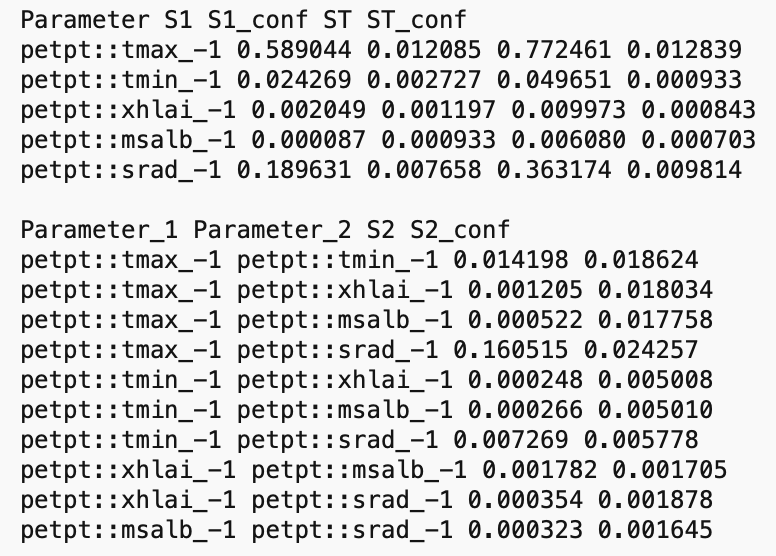
\includegraphics[width=.8\columnwidth]{sensitivity_indices}%
    \caption[PETPT Sensitivity Indices]{An example of all of the sensitivity indices returned by SALib for the PETPT evapo-transpiration model. This set of indices was created from a sample set of $50,000$ input samples for the PETPT model.}
\end{figure}
\FloatBarrier

In the figure we see that the $S_1$, $S_2$, and $S_T$ sensitivity indices are all computed and returned by this method of Sobol analysis as well as the $95\%$ confidence interval bounds for each value of each index.
We know that the ordered sensitivity indices computed using this method will sum to $1$ if all of the higher order indices are present \citep{sobol2001globalSA}.
We also know that the larger the value for any sensitivity index, the more of an affect the uncertainty in the corresponding input or set of inputs has on the uncertainty in model output.
Therefore we can use this information to inform our decisions about the model based on the uncertainty caused from model inputs.
For example, we can see that for the PETPT model, over $95\%$ of the uncertainty in the output of the model is caused by single or double variable interactions.
Not only is it very useful to have a scaled representation of causal uncertainty represent with each set of inputs, but the uniform scaling also allows for comparisons of scale across the inputs of multiple competing scientific models.

The total order index $S_T$ is also useful for decision making amongst our scientific models.
While this index does not sum to $1$ for the set of inputs, it is guaranteed to be greater than or equal to one, and allows us to see which input has the greatest compounded affect on output uncertainty.
We can use this information across models as well.
While we cannot compare scales across models without a normalizing factor, we can easily produce categorical comparisons across models of which inputs have the highest total order affects.

In the following sections of this chapter several use cases of the sensitivity indices will be presented.
However, the Sobol analysis method also returns useful information about the confidence in the estimate for each sensitivity index.
This information can be used to empirically determine if enough samples were included for the analysis to be successful.
A simple metric to use for this purpose is to have a cutoff for the largest confidence interval size.
If a confidence interval is returned that is larger than that maximum size, then add more samples from the Sobol sequence and rerun the analysis phase.
The SMS pipeline includes the usage of this technique to ensure that the sensitivity indices being used for analysis are sufficiently descriptive of the competing models.

\subsection{Model Output Surface\label{sec:out_surf}}
Although the sensitivity indices for a given scientific model are able to provide information on what input variables cause the most uncertainty upon the model output they do not provide any information about how the model output varies as a set of input variables varies.
However, this information is likely valuable to modelers as it will aid in their ability to distinguish between models based on the functional form of their outputs as a function of the most variable inputs.
To accomplish this goal, I created a new method that creates a plot of the output variable as a function of the two most sensitive inputs based upon the results from sensitivity analysis.
I refer to these new plots as a Model Output Surface (MOS) plot.

A MOS plot is a 3D plot where the z-axis is the output variable of a model and the remaining axes are input variables.
A MOS plot consists of the plotted outputs over a predefined range for each of the two inputs which creates a smooth surface object in three dimensions.
Evaluation to create this surface is done using a mesh grid of finite points.
Extrapolation between point evaluations can then be conducted to create the smooth surface visualization.
As expected, a higher number of input samples over the same input space range will lead to a smoother surface that is a more accurate representation of the true output surface for the input pair.
In this section I will cover the process of selecting which input variables to study with MOS plots, how to set values for the additional inputs not under study, and how to efficiently perform the evaluations necessary to generate a MOS plot.

\subsubsection{Input Variable Selection\label{sec:inp_var_sel}}
Most models will have more than two input variables and thus when creating a MOS plot a decision must be made about which two input variables should be varied during output surface creation. Generally speaking, for a model with $N$ input variables, a user could generate $\frac{N(N+1)}{2}$ plots to expose all possible pairs of variable interactions and examine how those interactions affect the output surface. For most sizes of $N$ this study is likely to not be computationally feasible, and modelers are unlikely to desire to view such a large number of output plots when performing model selection. A better use-case for MOS plots would be to showcase the pairs of variables that have the greatest combined affect on the model output.

In order to accomplish this task we need a way to rank the pairs of inputs in order of how greatly they affect model output. Fortunately we can attain this ranking directly from the second order sensitivity index, $S_2$. Utilizing the $S_2$ index as our ranking schema we can either create MOS plots for the top $k$ variable pairs, or we can use a threshold cutoff and create MOS plots for all pairs on input variables that exceed this cutoff. An appropriate cutoff could be a pre-defined value, or it could be based upon a difference between neighboring values of the sorted $S_2$ indices. An example of such a cutoff would be to generate MOS plots for all input pairs, until seeing a drop in $S_2$ index score of at least an order of magnitude.

It is important to note that utilizing the $S_2$ index is not the only way to select which input pairs to generate a MOS plot for, and is likely not the only metric of interest to modelers. If we have additional information, such as which inputs can be most or least accurately measured by the modelers then we may want to generate MOS plots for the modelers based upon this criterion so they can observe how output varies for input variables that they can measure well, vs those that they can measure poorly. This will becomes more important for model selection when competing models have differing sets of inputs, some of which may be easier or harder to measure than others.

\subsubsection{Input parameter estimation\label{sec:inp_param_est}}
Once the input variables for a given MOS plot are selected, the remaining inputs must have values assigned to them to allow for the model to be evaluated for MOS plot generation. To avoid confusion, I will refer to this set of input variables that will no longer be varied as the input parameters for the model.

There are many options present for assigning values to each of the input parameters. Unfortunately the nature of models also demands that either one or few values be chosen for each of the input parameters due to the high number of input parameters that are likely to be present. Even if we wished to allow for only two values for each input parameter, and wanted to study all possible combinations of them then for a set of $N$ input parameters we would generate $2^N$ MOS plots. Expecting modelers to review this many MOS plots goes against the idea of summarizing model behavior. This entails that a single set of values for the input parameters should be selected.

The task of input parameter estimation is now the task of finding the best-fit set of input parameters for a MOS plot. For each parameter we know that we have a range of values that were used for the parameter during analysis. From this information we can define that the best-fit for an input parameter is the Maximum Likelihood Estimate (MLE) over the range. The MLE is a useful estimate for each input parameter since the ranges are included for each parameter. However, if observational data were present, then it would be possible to use the Maximum A Priori (MAP) estimate as the setting for our input parameters.

\subsubsection{Surface Generation and Evaluation\label{sec:surf_usage}}
Once the decisions for the input variables to study and the preset parameter values to use have been made a MOS plot is easy to generate.
Generation requires model evaluation over large numbers of sets of inputs.
Since the plot itself takes the form of a meshgrid the amount of required evaluations will scale as expected for a meshgrid structure.
This means that if we want to study $1,000$ examples of each of the two variables under study we will need $1,000,000$ total evaluations.
Luckily this computation can be done efficiently using PyTorch tensor computation.
Once the evaluations are completed a MOS plot can be easily rendered and will appear interactively for the modelers. Below is an example of a MOS plot that would be presented for a modeler interested in working with the PETPT evapo-transpiration model.

\FloatBarrier
\begin{figure}[!htbp]
    \label{mos_plot_ex}
    \centering
    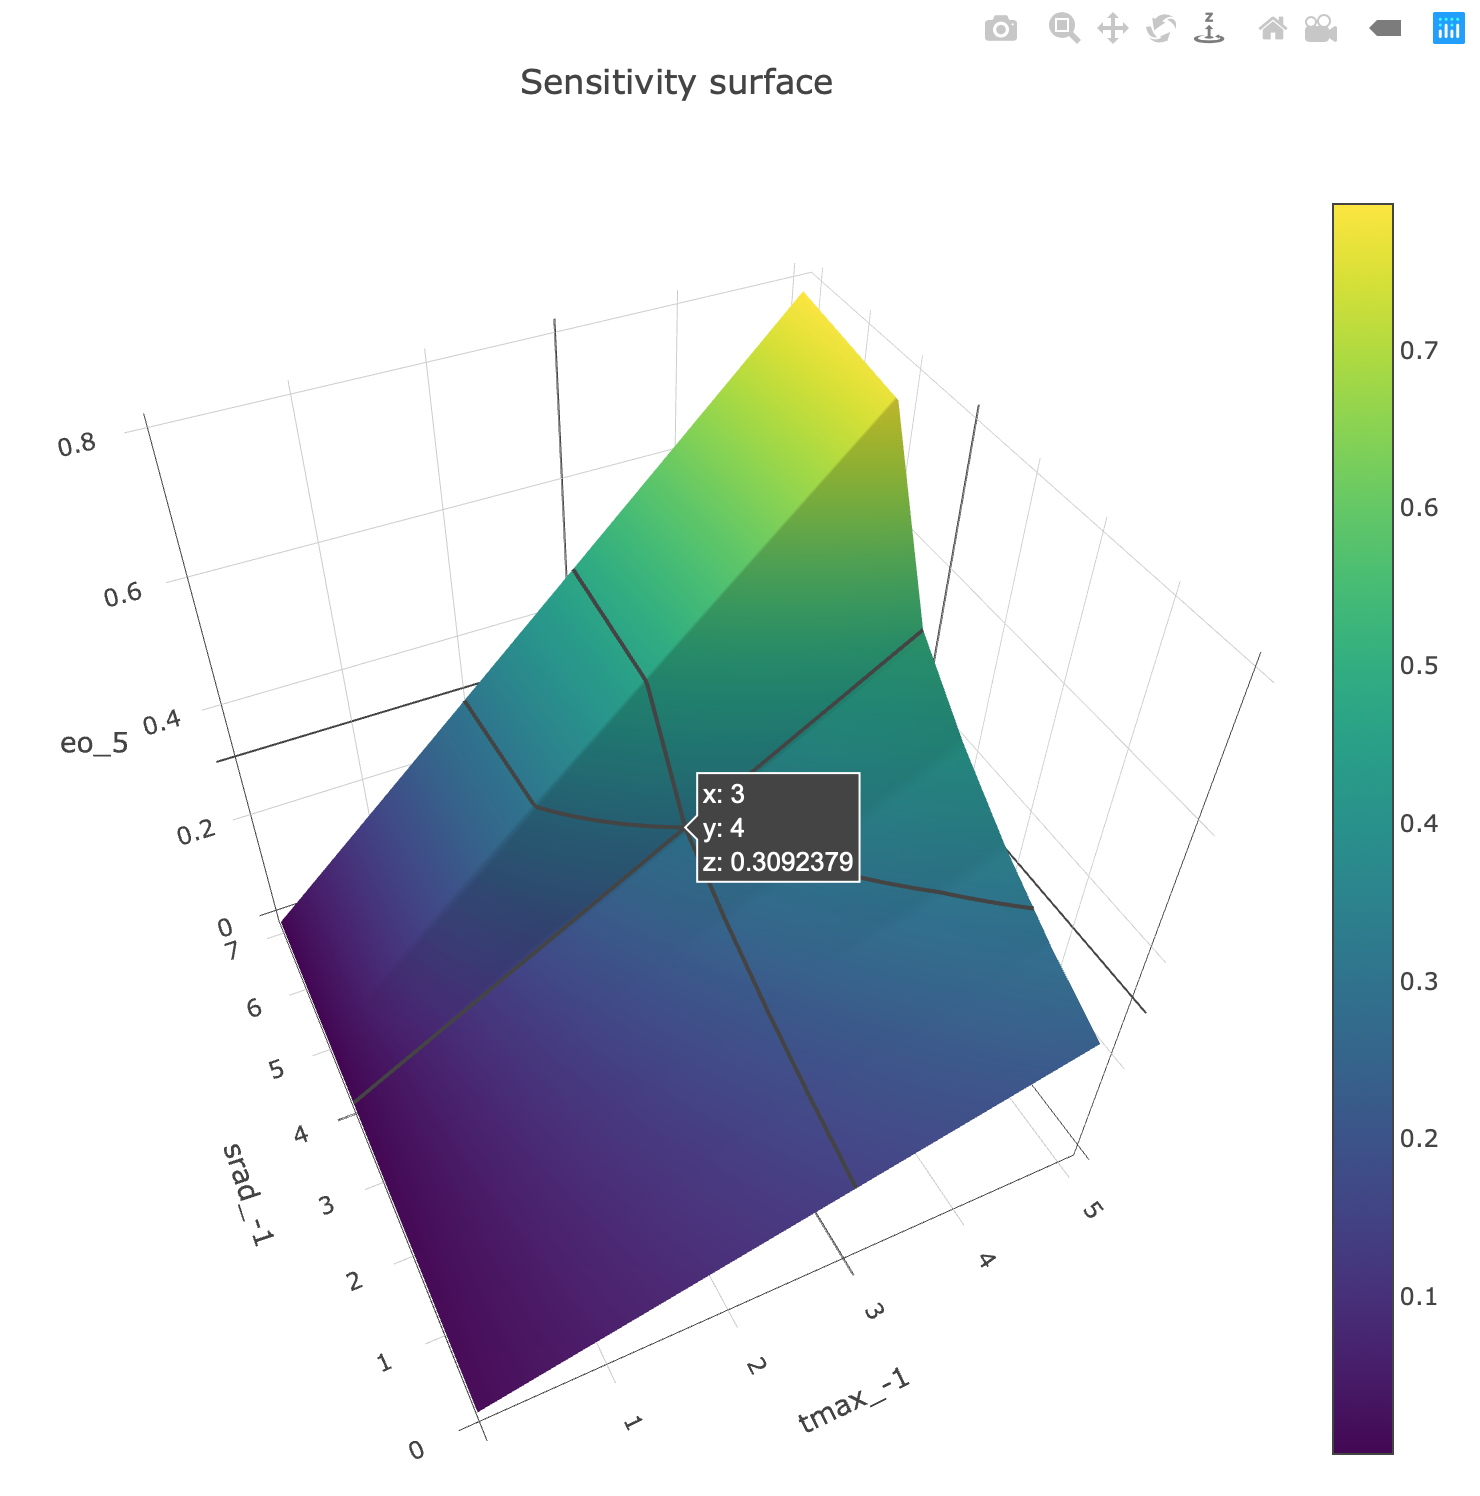
\includegraphics[width=.8\columnwidth]{sensitivity_surface}%
    \caption[PETPT Example MOS Plot]{An example of a MOS plot for the PETPT evapo-transpiration model. In this plot the two variables under study are solar radiation and the maximum temperature. Notice that these two variables covary and their variance greatly affects the shape of the model output surface.}
\end{figure}
\FloatBarrier

\subsection{Model Report Generation\label{sec:report_gen}}
Utilizing the information provided by the sensitivity indices of a model allows the SMS pipeline to gain insight about how the uncertainty in the output of the model is caused by the various inputs of the model.
However, this information alone is likely still too opaque to be useful to modelers when selecting a model for an experiment.
Ultimately the task of model selection comes down to an optimization problem for modelers based upon the desires they have for a models performance.
These tasks will likely differ between different modelers, but will almost certainly have some common themes.
In order to make the SMS pipeline as useful as possible to modelers we seek to provide modelers with the direct information from the sensitivity indices and also to provide them with useful abstractions created from the sensitivity indices that further differentiate competing models.
In this section I define the information contained in a model report that aims to differentiate two models so that modelers can perform their own model selection.

\subsubsection{Minimizing Measurement Error\label{sec:min_measure_error}}
When a modeler uses a model in an experiment they will need some method of collecting data for the inputs.
In almost all cases this immediately requires a modelers to address the question of: "how confident are you in your ability to measure input phenomena $x$?"
A modeler will likely want to select a model whose output is least sensitive to errors in measurements from the inputs that they are least able to measure accurately.
Only the modeler is aware of the measurement error associated with the devices used to measure each of their inputs; however, the information recovered in the sensitivity indices can be combined with the measurement error of each input to give the modeler a clear view of which model will perform best for them based upon minimizing the impact of measurement error.
Therefore, providing the sensitivity index information in an interpretable table as part of the model report is crucial for modelers.

\subsubsection{Cross-model Output Surface Examination \label{sec:multi_mod_surface}}
The sensitivity indices give a clear picture of which inputs or sets of inputs contribute the greatest amount of uncertainty to the model output.
Comparing sensitivity indices across the shared inputs of multiple models allows us to see where different models have the greatest amount of uncertainty.
However, this is still a summary statistic of the variance in model output caused by variance in the inputs.
While summary statistics are sufficient for some use cases, many modelers will likely want to base their model selection decision on the differences in shape of the model output for key variables that are shared between competing models.

This information can be provided to the modelers by the SMS pipeline in the form of comparative MOS plots, one per model, for given pairs of shared input variables that are of interest to the modelers.
These comparative MOS plots allow modelers to diagnose the functional differences in how two models differ based upon each individual models input variables of highest sensitivity, or based upon a shared set of input variables that have the highest combined sensitivity between the two models.
Modelers would be able to observe these surfaces without the aid of the SMS pipeline; however, without the information extracted from sensitivity analysis during the SMS pipeline modelers would need to generate MOS plots for every possibly set of input pairs.
The SMS pipeline removes this burden upon modelers by discovering which pairs of inputs are the most crucial to focus upon and automatically presenting those to modelers so that they can make expedient decisions amongst competing scientific models.

% \chapter{METHODS FOR INFORMED MODEL SELECTION\label{chapter:selection}}

Some intro about the task of selecting a model given the information from model analysis

\section{Model report generation\label{sec:report_gen}}

Some text

\section{Input space partitioning\label{sec:input_partition}}

Some text

\chapter{CONCLUSIONS AND FUTURE WORK\label{chapter:conc_and_future}}
In order to address the problem of model choice and to enable the process of model composition, domain modelers need access to implementations of models that are executable, analyzable, comparable, augmentable, and extendable.
Domain modelers also benefit from these implementations of models being as free from error as possible.
In order to develop model implementations that fit these criteria research efforts focused on assisting domain modelers have begun to focus on the problem of model extraction and assembly.
Current research efforts have focused on extracting models from unstructured as well as structured data sources, such as published text and formal \textit{datums}, and utilizing knowledge bases to assemble the extracted information into executable models.

In this thesis we introduced the components of the AutoMATES pipeline that provide input data to UMAF, including the translation of source code into an imperative intermediate representation and the extraction of variable grounding information from text and equation sources.
Afterwards we outlined the algorithm required to translate the imperative intermediate representation of a scientific model into the dataflow representation of a scientific model used as the basis for a GrFN, and showed how the variables in the GrFN could then be easily linked to real-world phenomena via variable grounding.
GrFNs were then shown to be executable by introducing the algorithms necessary to efficiently execute sets of inputs.
In particular, the algorithm that enables the extraction of a GrFN execution stack to ensure the proper execution order of the computations contained in a GrFN was introduced.
The structure of a GrFN, a function network, was then shown to be directly related to data structures from the family of probabilistic graphical models, in particular a dynamic bayesian network.
This implies that it is possible to conduct statistical inference over GrFN models using the toolbox of graphical modeling, which shows that GrFNs can be analyzed and compared.
Finally language feature coverage analyses were conducted on UMAF that demonstrated the coverage of program structures by UMAF as well as the accuracy of model extraction/assembly by UMAF from source code into GrFN.

The final product from this thesis is a framework that increases access to high fidelity executable, analyzable, comparable, augmentable, and extendable models by extracting and assembling models found in source code along with supporting information from published texts and equations.
The AutoMATES project is still in its infancy, and the work described in this thesis can serve as a firm foundation for the continued development of UMAF to further enable domain modelers realize the full potential of scientific modeling.

\section{Future Work\label{sec:future_work}}
As mentioned in the section above, UMAF will requires further development to assist domain modelers to the largest degree possible.
Some limitations upon UMAF stem from limitations from other components of the AutoMATES pipeline, such as the lack of complete coverage of Fortran code idioms by the Program Analysis Pipeline.
In addition, there are limitations that stem from a need to continue development of the algorithms and methods necessary to translate imperative source code into a GrFN.
In this section, we describe the future work that is necessary to resolve the current limitations of UMAF.

\subsection{Converting Complex Control Flow Structures \label{sec:early_exit}}
GrFNs are dataflow programs, and this means that they represent models as a flow of data, free from the control flow structures that are normally associated with imperative programs.
Currently UMAF is capable of converting many control flow structures, including conditionals, function calls, and loops into a dataflow form.
These forms of control flow that are supported by UMAF all behave as basic blocks that have one point of entry and one point of exit for any scope that they define.
However, UMAF does not yet support more complex forms of control flow that correspond to multiple points of exit or entry.
Some examples of such control structures are multiple returns from a function, break/continue statements inside of loops, and error handling in straight-line code.
Along with these issues comes the issue of exiting from nested scope layers, such as the presence of a conditional return statement in a loop that is contained in a function.
These structures present challenges to UMAF that will require the translation process of programs to GrFN to be extended.
In order to handle a wide range of scientific source code developed by a large array of domain experts with varying programming styles we will extend the translation process of GrFN presented in this thesis to handle the complex control flow styles discussed above and others that are discovered during the course of the AutoMATES project.

\subsection{Handling Complex Data Types \label{sec:complex_types}}
Currently, the UMAF framework is able to represent variables in GrFN that are derived from primitive data types.
These types include numeric types such as integers and floating point numbers, as well as non-numeric primitives such as booleans and strings.
However, programs often include complex types as well as a method of data management.
Examples of complex types include arrays, hash maps, and user-defined structs.
These complex types are all composed of primitive types that hold information that is likely grounded to real-world phenomena.
In order to include support for models that include these data types, the specification for GrFNs must be extended to incorporate complex types as variables.
This task includes determining how to represent complex types in a GrFN, as well as determining how to represent the access of variable fields in a complex type whether for getting, storing, or updating values.

\subsection{Temporary Variable Detection\label{sec:temp_vars}}
Currently UMAF assumes that all variables provided in a source code program correspond to real-world phenomena.
While this assumption may be true for some models, it is certainly the case that programmers and domain experts can utilize temporary variables that do not directly correspond to real-world phenomena.
This presents UMAF with the challenge of detecting which variables described in source code do directly correlate to real-world phenomena.
To address this challenge we will utilize more information from the text and equation reading modules of AutoMATES to discover which variables in the source code for a model are in fact real-world phenomena.
A trivial first pass to solve this problem is to utilize the results from variable grounding, but this solution can be extended by using information from equation reading to analyze the functional form of the computations in the source code to determine where temporary variables may exist.
Incorporating this step into UMAF will allow for the removal of temporary variables before the wiring and grounding processes begin and result in a more accurate model representation of the real-world system.

\subsection{Variable Domain Detection\label{sec:var_domain_detection}}
One key issue that has not been addressed in this thesis so far is the issue of discovering the domain limitations of input variables in computation graphs.
Scientific models that are expressed in code are generally unlimited in terms of their functional form.
However certain mathematical functions place limits on the domains of variables used in their computation.
A classic example of this can be found in the source code for the PETASCE evapotranspiration model found in Appendix~\ref{sec:asce_src_code}.
In line $40$ we find the computation of variable \textit{RHMIN} depends upon variables \textit{EA} and \textit{EMAX}.
From the functional form of the computation we can observe that \textit{EMAX} cannot equal zero, otherwise a division by zero error would occur during computation.
That is a constraint upon the domain for \textit{EMAX}; however, \textit{EMAX} is not an input for the PETASCE model but is the result from a computation from inputs to the PETASCE model.
This shows that one task required for domain detection is for constraints from inner variables computed in the computations of the model, such as \textit{EMAX}, to be propagated backwards to the input variables responsible for their computation.
This task is necessary to support model analysis upon the GrFNs produced by UMAF, since a key portion of analysis is to sample over the domains of the inputs.
Therefore, accomplishing variable domain detection is a necessary next step to ensure the usefulness of GrFNs created by UMAF.


% Include the various appendices
% \appendix
% \chapter{Evapo-Transpiration Model Source Code\label{appendix:a}}

\section{Priestley Taylor PET Model Source Code \label{sec:pt_src_code}}
\begin{minted}
  [
    fontsize=\footnotesize,
    framesep=1mm,
    baselinestretch=1.0,
    linenos
  ]
  {fortran}
C=======================================================================
      SUBROUTINE PETPT(
     &    MSALB, SRAD, TMAX, TMIN, XHLAI,                 !Input
     &    EO)                                             !Output
      IMPLICIT NONE
!     INPUT VARIABLES:
      REAL MSALB, SRAD, TMAX, TMIN, XHLAI
!     OUTPUT VARIABLES:
      REAL EO
!     LOCAL VARIABLES:
      REAL ALBEDO, EEQ, SLANG, TD

      TD = 0.60*TMAX+0.40*TMIN
      IF (XHLAI .LE. 0.0) THEN
        ALBEDO = MSALB
      ELSE
        ALBEDO = 0.23-(0.23-MSALB)*EXP(-0.75*XHLAI)
      ENDIF
      SLANG = SRAD*23.923
      EEQ = SLANG*(2.04E-4-1.83E-4*ALBEDO)*(TD+29.0)
      EO = EEQ*1.1
      IF (TMAX .GT. 35.0) THEN
        EO = EEQ*((TMAX-35.0)*0.05+1.1)
      ELSE IF (TMAX .LT. 5.0) THEN
        EO = EEQ*0.01*EXP(0.18*(TMAX+20.0))
      ENDIF
      EO = MAX(EO,0.0001)
      RETURN
      END SUBROUTINE PETPT
!-----------------------------------------------------------------------
!     PETPT VARIABLES:
!-----------------------------------------------------------------------
! ALBEDO  Reflectance of soil-crop surface (fraction)
! EEQ     Equilibrium evaporation (mm/d)
! EO      Potential evapotranspiration rate (mm/d)
! MSALB   Soil albedo with mulch and soil water effects (fraction)
! SLANG   Solar radiation
! SRAD    Solar radiation (MJ/m2-d)
! TD      Approximation of average daily temperature (C)
! TMAX    Maximum daily temperature (C)
! TMIN    Minimum daily temperature (C)
! XHLAI   Leaf area index (m2[leaf] / m2[ground])
!-----------------------------------------------------------------------
!     END SUBROUTINE PETPT
C=======================================================================
\end{minted}

\section{ASCE PET Model Source Code \label{sec:asce_src_code}}
\begin{minted}
  [
    fontsize=\footnotesize,
    framesep=1mm,
    baselinestretch=1.0,
    linenos
  ]
  {fortran}
C=======================================================================
      SUBROUTINE PETASCE(
     &        CANHT, DOY, MSALB, MEEVP, SRAD, TDEW,       !Input
     &        TMAX, TMIN, WINDHT, WINDRUN, XHLAI,         !Input
     &        XLAT, XELEV,                                !Input
     &        EO)                                         !Output
      IMPLICIT NONE
      SAVE
!     INPUT VARIABLES:
      REAL CANHT, MSALB, SRAD, TDEW, TMAX, TMIN, WINDHT, WINDRUN
      REAL XHLAI, XLAT, XELEV
      INTEGER DOY
      CHARACTER*1 MEEVP
!     OUTPUT VARIABLES:
      REAL EO
!     LOCAL VARIABLES:
      REAL TAVG, PATM, PSYCON, UDELTA, EMAX, EMIN, ES, EA, FC, FEW, FW
      REAL ALBEDO, RNS, PIE, DR, LDELTA, WS, RA1, RA2, RA, RSO, RATIO
      REAL FCD, TK4, RNL, RN, G, WINDSP, WIND2m, Cn, Cd, KCMAX, RHMIN
      REAL WND, CHT
      REAL REFET, SKC, KCBMIN, KCBMAX, KCB, KE, KC
!-----------------------------------------------------------------------
!     ASCE Standardized Reference Evapotranspiration
!     Average temperature (ASCE Standard Eq. 2)
      TAVG = (TMAX + TMIN) / 2.0 !deg C
!     Atmospheric pressure (ASCE Standard Eq. 3)
      PATM = 101.3 * ((293.0 - 0.0065 * XELEV)/293.0) ** 5.26 !kPa
!     Psychrometric constant (ASCE Standard Eq. 4)
      PSYCON = 0.000665 * PATM !kPa/deg C
!     Slope of the saturation vapor pressure-temperature curve
!     (ASCE Standard Eq. 5)                                !kPa/degC
      UDELTA = 2503.0*EXP(17.27*TAVG/(TAVG+237.3))/(TAVG+237.3)**2.0
!     Saturation vapor pressure (ASCE Standard Eqs. 6 and 7)
      EMAX = 0.6108*EXP((17.27*TMAX)/(TMAX+237.3)) !kPa
      EMIN = 0.6108*EXP((17.27*TMIN)/(TMIN+237.3)) !kPa
      ES = (EMAX + EMIN) / 2.0                     !kPa
!     Actual vapor pressure (ASCE Standard Eq. 8)
      EA = 0.6108*EXP((17.27*TDEW)/(TDEW+237.3)) !kPa
!     RHmin (ASCE Standard Eq. 13, RHmin limits from FAO-56 Eq. 70)
      RHMIN = MAX(20.0, MIN(80.0, EA/EMAX*100.0))
!     Net shortwave radiation (ASCE Standard Eq. 16)
      IF (XHLAI .LE. 0.0) THEN
        ALBEDO = MSALB
      ELSE
        ALBEDO = 0.23
      ENDIF
      RNS = (1.0-ALBEDO)*SRAD !MJ/m2/d
!     Extraterrestrial radiation (ASCE Standard Eqs. 21,23,24,27)
      PIE = 3.14159265359
      DR = 1.0+0.033*COS(2.0*PIE/365.0*DOY) !Eq. 23
      LDELTA = 0.409*SIN(2.0*PIE/365.0*DOY-1.39) !Eq. 24
      WS = ACOS(-1.0*TAN(XLAT*PIE/180.0)*TAN(LDELTA)) !Eq. 27
      RA1 = WS*SIN(XLAT*PIE/180.0)*SIN(LDELTA) !Eq. 21
      RA2 = COS(XLAT*PIE/180.0)*COS(LDELTA)*SIN(WS) !Eq. 21
      RA = 24.0/PIE*4.92*DR*(RA1+RA2) !MJ/m2/d Eq. 21
!     Clear sky solar radiation (ASCE Standard Eq. 19)
      RSO = (0.75+2E-5*XELEV)*RA !MJ/m2/d
!     Net longwave radiation (ASCE Standard Eqs. 17 and 18)
      RATIO = SRAD/RSO
      IF (RATIO .LT. 0.3) THEN
        RATIO = 0.3
      ELSEIF (RATIO .GT. 1.0) THEN
        RATIO = 1.0
      END IF
      FCD = 1.35*RATIO-0.35 !Eq 18
      TK4 = ((TMAX+273.16)**4.0+(TMIN+273.16)**4.0)/2.0 !Eq. 17
      RNL = 4.901E-9*FCD*(0.34-0.14*SQRT(EA))*TK4 !MJ/m2/d Eq. 17
!     Net radiation (ASCE Standard Eq. 15)
      RN = RNS - RNL !MJ/m2/d
!     Soil heat flux (ASCE Standard Eq. 30)
      G = 0.0 !MJ/m2/d
!     Wind speed (ASCE Standard Eq. 33)
      WINDSP = WINDRUN * 1000.0 / 24.0 / 60.0 / 60.0 !m/s
      WIND2m = WINDSP * (4.87/LOG(67.8*WINDHT-5.42))
      Cn = 0.0
      Cd = 0.0
      IF (MEEVP .EQ. 'A') THEN
        Cn = 1600.0
        Cd = 0.38
      ELSE IF (MEEVP .EQ. 'G') THEN
        Cn = 900.0
        Cd = 0.34
      END IF
!     Standardized reference evapotranspiration (ASCE Standard Eq. 1)
      REFET =0.408*UDELTA*(RN-G)+PSYCON*(Cn/(TAVG+273.0))*WIND2m*(ES-EA)
      REFET = REFET/(UDELTA+PSYCON*(1.0+Cd*WIND2m)) !mm/d
      REFET = MAX(0.0001, REFET)
!     FAO-56 dual crop coefficient approach
!     Basal crop coefficient (Kcb)
!     Also similar to FAO-56 Eq. 97
!     KCB is zero when LAI is zero
      SKC = 0.8
      KCBMIN = 0.3
      KCBMAX = 1.2
      IF (XHLAI .LE. 0.0) THEN
         KCB = 0.0
      ELSE
         !DeJonge et al. (2012) equation
         KCB = MAX(0.0,KCBMIN+(KCBMAX-KCBMIN)*(1.0-EXP(-1.0*SKC*XHLAI)))
      ENDIF
      !Maximum crop coefficient (Kcmax) (FAO-56 Eq. 72)
      WND = MAX(1.0,MIN(WIND2m,6.0))
      CHT = MAX(0.001,CANHT)
      KCMAX = 0.5           ! HACK: Guarantees greater that KCBMIN
      IF (MEEVP .EQ. 'A') THEN
        KCMAX = MAX(1.0,KCB+0.05)
      ELSE IF (MEEVP .EQ. 'G') THEN
        KCMAX = MAX((1.2+(0.04*(WND-2.0)-0.004*(RHMIN-45.0))
     &                      *(CHT/3.0)**(0.3)),KCB+0.05)
      END IF
      !Effective canopy cover (fc) (FAO-56 Eq. 76)
      IF (KCB .LE. KCBMIN) THEN
         FC = 0.0
      ELSE
         FC = ((KCB-KCBMIN)/(KCMAX-KCBMIN))**(1.0+0.5*CANHT)
      ENDIF
      !Exposed and wetted soil fraction (FAO-56 Eq. 75)
      !Unresolved issue with FW (fraction wetted soil surface).
      !Some argue FW should not be used to adjust demand.
      !Rather wetting fraction issue should be addressed on supply side.
      !Difficult to do with a 1-D soil water model
      FW = 1.0
      FEW = MIN(1.0-FC,FW)
      !Potential evaporation coefficient (Ke) (Based on FAO-56 Eq. 71)
      !Kr = 1.0 since this is potential Ke. Model routines handle stress
      KE = MAX(0.0, MIN(1.0*(KCMAX-KCB), FEW*KCMAX))
      !Potential evapotranspiration (FAO-56 Eq. 69)
      EO = (KCB + KE) * REFET
      EO = MAX(EO,0.0001)
      RETURN
      END SUBROUTINE PETASCE
!-------------------------------------------------------------------
\end{minted}


% Switch the spacing to single-spaced for the references
\renewcommand{\baselinestretch}{1}		% changing the value
\small\normalsize										% switch size to make the value take

% Create the References list
\bibliographystyle{uabibnat}
\bibliography{bibliography}

\end{document}
